% Template Header
\documentclass[12pt]{article}
\usepackage{graphicx}
\usepackage[a4paper,margin=15mm]{geometry}
\usepackage[table]{xcolor}
\usepackage{tikz}
\usepackage{lastpage}
\usepackage{fancyhdr}
\usepackage{hyperref}


\renewcommand{\familydefault}{\sfdefault}

\parskip 7.2pt

\def\doctitle{Gravity Model Report}
\def\docauthor{Longfei Zhao, Simon Perreault \& Jason Michel Lambert}
\def\docdate{\today}
\def\docrevision{DRAFT}
\def\doctype{X?.?-00\_Documentation R01}
\def\docconfidentiality{PR37 7DOF}
\def\docfilename{Gravity Model Report.pdf}

\hypersetup{
    colorlinks,
    citecolor=black,
    filecolor=black,
    linkcolor=black,
    urlcolor=black
}
% End Template Header

\usepackage{caption} % two figures in a row

\usepackage[cmex10]{amsmath}
\usepackage{multirow}
\usepackage{makecell}
\usepackage{soul}
\usepackage{array}
\usepackage{color}
\usepackage{transparent}
%% Utilisation de natbib pour les citations et la bibliographie.
\usepackage{natbib}
%% Autres packages.
\usepackage{amsmath,color,soulutf8,longtable,colortbl,setspace,ifthen,xspace,url,pdflscape}
\usepackage{epstopdf}


\begin{document}

% To use this cover, you need to have the following in your preamble
%
% \documentclass[12pt]{article}
% \usepackage{graphicx}
% \usepackage[a4paper,margin=15mm]{geometry}
% \usepackage[table]{xcolor}
% \usepackage{tikz}
% \usepackage{lastpage}
% \usepackage{fancyhdr}
%
% And you need to define these parameters:
%
% \def\doctitle{TITLE}
% \def\docauthor{AUTHOR}
% \def\docdate{DATE}                % Note: \today could be used for DATE
% \def\docrevision{REVISION}        % For example `Revision 01`
% \def\doctype{TYPE}                % For example `F7.3-02_Product Requirement R01`
% \def\docconfidentiality{CONF}     % For example `Internal Use Only`, or `Confidential`
% \def\docfilename{FILENAME}
%
% This cover was designed with this family of fonts, and may be out of shape with a different font:
%
% \renewcommand{\familydefault}{\sfdefault}
%
% The Kinova logo must be present in images/logo_kinova.pdf, and a version with
% white font instead of black, in images/logo_kinova_inv.pdf.
% If you have an svg, you can convert it first to eps with Inkscape:
%
%     inkscape file.svg --export-eps=file.eps
%
% and then from eps to pdf:
%
%     epstopdf --outfile=file.pdf file.eps
%
% To use this cover, after \begin{document}, simply do:
%
%     % To use this cover, you need to have the following in your preamble
%
% \documentclass[12pt]{article}
% \usepackage{graphicx}
% \usepackage[a4paper,margin=15mm]{geometry}
% \usepackage[table]{xcolor}
% \usepackage{tikz}
% \usepackage{lastpage}
% \usepackage{fancyhdr}
%
% And you need to define these parameters:
%
% \def\doctitle{TITLE}
% \def\docauthor{AUTHOR}
% \def\docdate{DATE}                % Note: \today could be used for DATE
% \def\docrevision{REVISION}        % For example `Revision 01`
% \def\doctype{TYPE}                % For example `F7.3-02_Product Requirement R01`
% \def\docconfidentiality{CONF}     % For example `Internal Use Only`, or `Confidential`
% \def\docfilename{FILENAME}
%
% This cover was designed with this family of fonts, and may be out of shape with a different font:
%
% \renewcommand{\familydefault}{\sfdefault}
%
% The Kinova logo must be present in images/logo_kinova.pdf, and a version with
% white font instead of black, in images/logo_kinova_inv.pdf.
% If you have an svg, you can convert it first to eps with Inkscape:
%
%     inkscape file.svg --export-eps=file.eps
%
% and then from eps to pdf:
%
%     epstopdf --outfile=file.pdf file.eps
%
% To use this cover, after \begin{document}, simply do:
%
%     % To use this cover, you need to have the following in your preamble
%
% \documentclass[12pt]{article}
% \usepackage{graphicx}
% \usepackage[a4paper,margin=15mm]{geometry}
% \usepackage[table]{xcolor}
% \usepackage{tikz}
% \usepackage{lastpage}
% \usepackage{fancyhdr}
%
% And you need to define these parameters:
%
% \def\doctitle{TITLE}
% \def\docauthor{AUTHOR}
% \def\docdate{DATE}                % Note: \today could be used for DATE
% \def\docrevision{REVISION}        % For example `Revision 01`
% \def\doctype{TYPE}                % For example `F7.3-02_Product Requirement R01`
% \def\docconfidentiality{CONF}     % For example `Internal Use Only`, or `Confidential`
% \def\docfilename{FILENAME}
%
% This cover was designed with this family of fonts, and may be out of shape with a different font:
%
% \renewcommand{\familydefault}{\sfdefault}
%
% The Kinova logo must be present in images/logo_kinova.pdf, and a version with
% white font instead of black, in images/logo_kinova_inv.pdf.
% If you have an svg, you can convert it first to eps with Inkscape:
%
%     inkscape file.svg --export-eps=file.eps
%
% and then from eps to pdf:
%
%     epstopdf --outfile=file.pdf file.eps
%
% To use this cover, after \begin{document}, simply do:
%
%     \input{kinovacover.tex}
%

\begin{titlepage}

  \vspace*{10mm}
  \begin{center}
    \Huge{\textbf{\doctitle}}

    \vspace*{15mm}
    \Large{\textbf{\docrevision}}

    \Large{\textbf{\docdate}}

    \vspace*{15mm}
    \textbf{By}

    \Large{\textbf{\docauthor}}
  \end{center}

  \vspace*{10mm}
  \hspace{-5cm}
  
\begin{tikzpicture}
    \draw[color=black,fill=black] (0,0) rectangle (50cm,5.5cm);
    \draw[color=cyan,fill=cyan] (0,5.5cm) rectangle (50cm,6cm);
  \end{tikzpicture}

  \vspace*{-50mm}

  \begin{center}
    
\includegraphics[width=10cm]{images/logo_kinova_inv}
  \end{center}

  \vspace*{20mm}
  \noindent
  \textbf{Warning}

  \noindent
  The information contained in this document is the property of Kinova. Except as
  specifically authorized in writing by Kinova, the holder of this document shall keep the
  information contained here confidential and shall protect same in whole or in part from
  disclosure and dissemination to third parties and use same for evaluation, operation and
  maintenance purposes only. This document is not an engagement of Kinova to develop,
  implement or design the product or techniques described here.

\end{titlepage}

\newpage

\setlength{\voffset}{-1in}
\setlength{\topmargin}{10pt}
\setlength{\headheight}{50pt}
\setlength{\footskip}{40pt}
\setlength{\textheight}{0.9\textheight}
\pagestyle{fancy}
\fancyhf{}
\fancyhead[L]{\color{gray}{\renewcommand{\arraystretch}{0.75}\begin{tabular}{l}
    \footnotesize \doctype - \doctitle \\
    \footnotesize Effective Date: \docdate \\
    \footnotesize \textbf{\docconfidentiality} \\
  \end{tabular}}
}
\fancyhead[R]{
\includegraphics[width=40mm]{images/logo_kinova}\vspace*{-15pt}}
\renewcommand{\headrulewidth}{0.5pt}
\fancyfoot[L]{\vspace*{-7pt}\color{gray}{\renewcommand{\arraystretch}{0.75}\begin{tabular}{l}
    \footnotesize \docfilename \\
    \footnotesize Printed: \docdate \\
  \end{tabular}}
}
\fancyfoot[R]{\footnotesize Page \thepage~of \pageref{LastPage}}
\renewcommand{\footrulewidth}{0.5pt}

%

\begin{titlepage}

  \vspace*{10mm}
  \begin{center}
    \Huge{\textbf{\doctitle}}

    \vspace*{15mm}
    \Large{\textbf{\docrevision}}

    \Large{\textbf{\docdate}}

    \vspace*{15mm}
    \textbf{By}

    \Large{\textbf{\docauthor}}
  \end{center}

  \vspace*{10mm}
  \hspace{-5cm}
  
\begin{tikzpicture}
    \draw[color=black,fill=black] (0,0) rectangle (50cm,5.5cm);
    \draw[color=cyan,fill=cyan] (0,5.5cm) rectangle (50cm,6cm);
  \end{tikzpicture}

  \vspace*{-50mm}

  \begin{center}
    
\includegraphics[width=10cm]{images/logo_kinova_inv}
  \end{center}

  \vspace*{20mm}
  \noindent
  \textbf{Warning}

  \noindent
  The information contained in this document is the property of Kinova. Except as
  specifically authorized in writing by Kinova, the holder of this document shall keep the
  information contained here confidential and shall protect same in whole or in part from
  disclosure and dissemination to third parties and use same for evaluation, operation and
  maintenance purposes only. This document is not an engagement of Kinova to develop,
  implement or design the product or techniques described here.

\end{titlepage}

\newpage

\setlength{\voffset}{-1in}
\setlength{\topmargin}{10pt}
\setlength{\headheight}{50pt}
\setlength{\footskip}{40pt}
\setlength{\textheight}{0.9\textheight}
\pagestyle{fancy}
\fancyhf{}
\fancyhead[L]{\color{gray}{\renewcommand{\arraystretch}{0.75}\begin{tabular}{l}
    \footnotesize \doctype - \doctitle \\
    \footnotesize Effective Date: \docdate \\
    \footnotesize \textbf{\docconfidentiality} \\
  \end{tabular}}
}
\fancyhead[R]{
\includegraphics[width=40mm]{images/logo_kinova}\vspace*{-15pt}}
\renewcommand{\headrulewidth}{0.5pt}
\fancyfoot[L]{\vspace*{-7pt}\color{gray}{\renewcommand{\arraystretch}{0.75}\begin{tabular}{l}
    \footnotesize \docfilename \\
    \footnotesize Printed: \docdate \\
  \end{tabular}}
}
\fancyfoot[R]{\footnotesize Page \thepage~of \pageref{LastPage}}
\renewcommand{\footrulewidth}{0.5pt}

%

\begin{titlepage}

  \vspace*{10mm}
  \begin{center}
    \Huge{\textbf{\doctitle}}

    \vspace*{15mm}
    \Large{\textbf{\docrevision}}

    \Large{\textbf{\docdate}}

    \vspace*{15mm}
    \textbf{By}

    \Large{\textbf{\docauthor}}
  \end{center}

  \vspace*{10mm}
  \hspace{-5cm}
  
\begin{tikzpicture}
    \draw[color=black,fill=black] (0,0) rectangle (50cm,5.5cm);
    \draw[color=cyan,fill=cyan] (0,5.5cm) rectangle (50cm,6cm);
  \end{tikzpicture}

  \vspace*{-50mm}

  \begin{center}
    
\includegraphics[width=10cm]{images/logo_kinova_inv}
  \end{center}

  \vspace*{20mm}
  \noindent
  \textbf{Warning}

  \noindent
  The information contained in this document is the property of Kinova. Except as
  specifically authorized in writing by Kinova, the holder of this document shall keep the
  information contained here confidential and shall protect same in whole or in part from
  disclosure and dissemination to third parties and use same for evaluation, operation and
  maintenance purposes only. This document is not an engagement of Kinova to develop,
  implement or design the product or techniques described here.

\end{titlepage}

\newpage

\setlength{\voffset}{-1in}
\setlength{\topmargin}{10pt}
\setlength{\headheight}{50pt}
\setlength{\footskip}{40pt}
\setlength{\textheight}{0.9\textheight}
\pagestyle{fancy}
\fancyhf{}
\fancyhead[L]{\color{gray}{\renewcommand{\arraystretch}{0.75}\begin{tabular}{l}
    \footnotesize \doctype - \doctitle \\
    \footnotesize Effective Date: \docdate \\
    \footnotesize \textbf{\docconfidentiality} \\
  \end{tabular}}
}
\fancyhead[R]{
\includegraphics[width=40mm]{images/logo_kinova}\vspace*{-15pt}}
\renewcommand{\headrulewidth}{0.5pt}
\fancyfoot[L]{\vspace*{-7pt}\color{gray}{\renewcommand{\arraystretch}{0.75}\begin{tabular}{l}
    \footnotesize \docfilename \\
    \footnotesize Printed: \docdate \\
  \end{tabular}}
}
\fancyfoot[R]{\footnotesize Page \thepage~of \pageref{LastPage}}
\renewcommand{\footrulewidth}{0.5pt}


\parindent = 0pt

\tableofcontents

\newpage

\section{Abstract}
% abstract
This report aims to provide a general review on the performance of the gravity model used on the PR37 surgical 7DOF arm MS7. The gravity model is originally designed as a standalone feature offline on PC (named \textbf{JointWrench\_PC} for convenience), and then integrated to real time system in robot base (named \textbf{JointWrench\_Base}). In PR37 arm, torque sensor data from each actuator (named \textbf{JointTorque\_Sensor}) will be used to evaluate gravity performance.

In this report, we will first compare JointWrench\_Base and JointWrench\_PC to confirm that the designed gravity model is well implemented in robot control system. After then, we will compare the component of torque along Z axis in JointWrench\_Base with JointTorque\_Sensor. Assuming that torque sensor reading is reliable, the difference between nominal and experimental joint torques should be below a certain threshold. This report will present all results and analysis regarding to the evaluation of gravity model. 

The tests in this report are designed for a MS7 robot set, which includes the 7DOF arm and IDM, no extra load. 

Robot configuration plays an important role in the gravity model. The pre-defined robot configurations can be divided in two groups. The first group includes robot configurations provided by Auris for different use cases. The second group includes robot configurations that maximize the load a certain joint. Therefore, the pre-defined robot configurations cover the general cases as well as the extreme cases. 



\newpage

\section{Test Setup}
% testSetup.tex

\subsection{Robot setup}

The base of PR37 robot is horizontally attached to a vertical pole. At its initial position (also defined as Pose11 in pre-defined robot configurations), the robot is fully extended and the torque load at each actuator sensor is ideally zero. The user should reset joint torque sensor if the data from torque sensor is needed.

\begin{figure}
	\begin{center}
				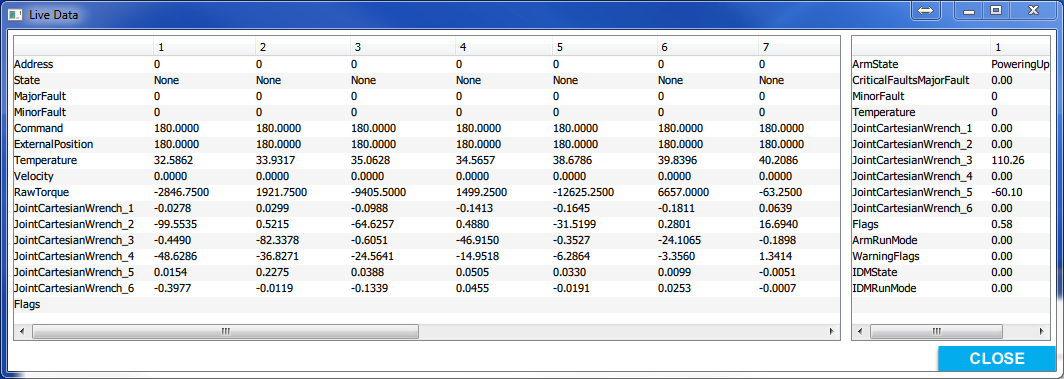
\includegraphics[width=0.9\textwidth]{./images/Pose11}%
		\caption{Test setup}
		\label{fig:pose11}%
	\end{center}
\end{figure}


\subsection{Pre-defined robot configurations}

At each pre-defined robot configuration, the sensor data will be recorded and compared with the gravity model output. Their difference will be used to evaluate the gravity model performance.  At different robot configurations, the torque at each actuator may vary widely. Therefore, the choice of robot configuration for gravity model evaluation is important. 
The pre-defined robot configurations used in this report can be categorized into two groups. 

\textbf{Group A}
In the first group (see in Table \ref{table-groupA}), the robot configurations are provided by Auris from some real user cases. The robot is in a normal operating condition, and these statuses present most common cases.

\begin{table}[]
	\centering
	\caption{Pre-defined Robot Configuration of Group A (Degrees)}
	\label{table-groupA}
	\begin{tabular}{|l|r|r|r|r|r|r|r|}
		\hline
		\textbf{} & \textbf{Joint1} & \textbf{Joint2} & \textbf{Joint3} & \textbf{Joint4} & \textbf{Joint5} & \textbf{Joint6} & \textbf{Joint7} \\ \hline
		\textbf{Pose 1}  & 115.00           & 236.85           & 138.20           & 264.09           & 63.00            & 235.28           & 155.28           \\ \hline
		\textbf{Pose 2}  & 140.00           & 245.42           & 90.92            & 281.41           & 353.62           & 295.06           & 265.40           \\ \hline
		\textbf{Pose 3}  & 293.00           & 137.05           & 220.52           & 87.40            & 217.98           & 307.70           & 103.13           \\ \hline
		\textbf{Pose 4}  & 10.00            & 176.73           & 147.59           & 43.32            & 142.68           & 275.00           & 205.12           \\ \hline
		\textbf{Pose 5}  & 85.00            & 255.93           & 141.29           & 236.09           & 65.84            & 228.26           & 130.50           \\ \hline
		\textbf{Pose 6}  & 140.00           & 205.51           & 96.12            & 275.16           & 313.20           & 260.62           & 229.57           \\ \hline
		\textbf{Pose 7}  & 120.00           & 240.31           & 140.20           & 239.88           & 66.74            & 239.24           & 115.38           \\ \hline
		\textbf{Pose 8}  & 285.00           & 113.25           & 129.73           & 289.67           & 7.89             & 195.54           & 83.44            \\ \hline
		\textbf{Pose 9}  & 285.00           & 121.22           & 234.46           & 131.94           & 356.65           & 77.01            & 227.27           \\ \hline
		\textbf{Pose 10} & 340.00           & 141.74           & 22.27            & 67.95            & 16.12            & 61.73            & 153.11           \\ \hline
	\end{tabular}
\end{table}



\textbf{Group B}
In the second group (see in Table \ref{table-groupB}), the robot configurations are defined to have a maximum load on one or several joints. Since there is no extra load on the robot end-effector, the load only takes robot arm and IDM into account. 


\begin{table}[]
	\centering
	\caption{Pre-defined Robot Configuration of Group B (Degrees)}
	\label{table-groupB}
	\begin{tabular}{|l|r|r|r|r|r|r|r|r|}
		\hline
		\textbf{}        & \textbf{Joint1} & \textbf{Joint2} & \textbf{Joint3} & \textbf{Joint4} & \textbf{Joint5} & \textbf{Joint6} & \textbf{Joint7} & \textbf{Maximum Load}        \\ \hline
		\textbf{Pose 11} & 180              & 180              & 180              & 180              & 180              & 180              & 180              & No load to all (Figure \ref{fig:pose11})         \\ \hline
		\textbf{Pose 12} & 270              & 180              & 180              & 180              & 180              & 180              & 180              & Joint 2, 4, 6, 7 (Figure \ref{fig:pose12}) \\ \hline
		\textbf{Pose 13} & 180              & 180              & 180              & 180              & 180              & 90               & 180              & Joint 5 (Figure \ref{fig:pose13})      \\ \hline
		\textbf{Pose 14} & 180              & 180              & 180              & 90               & 180              & 180              & 180              & Joint 3 (Figure \ref{fig:pose14})      \\ \hline
		\textbf{Pose 15} & 180              & 90               & 180              & 180              & 180              & 180              & 180              & Joint 1 (Figure \ref{fig:pose15})      \\ \hline
	\end{tabular}
\end{table}


\begin{figure}
	\centering
	\begin{minipage}{.5\textwidth}
		\centering
		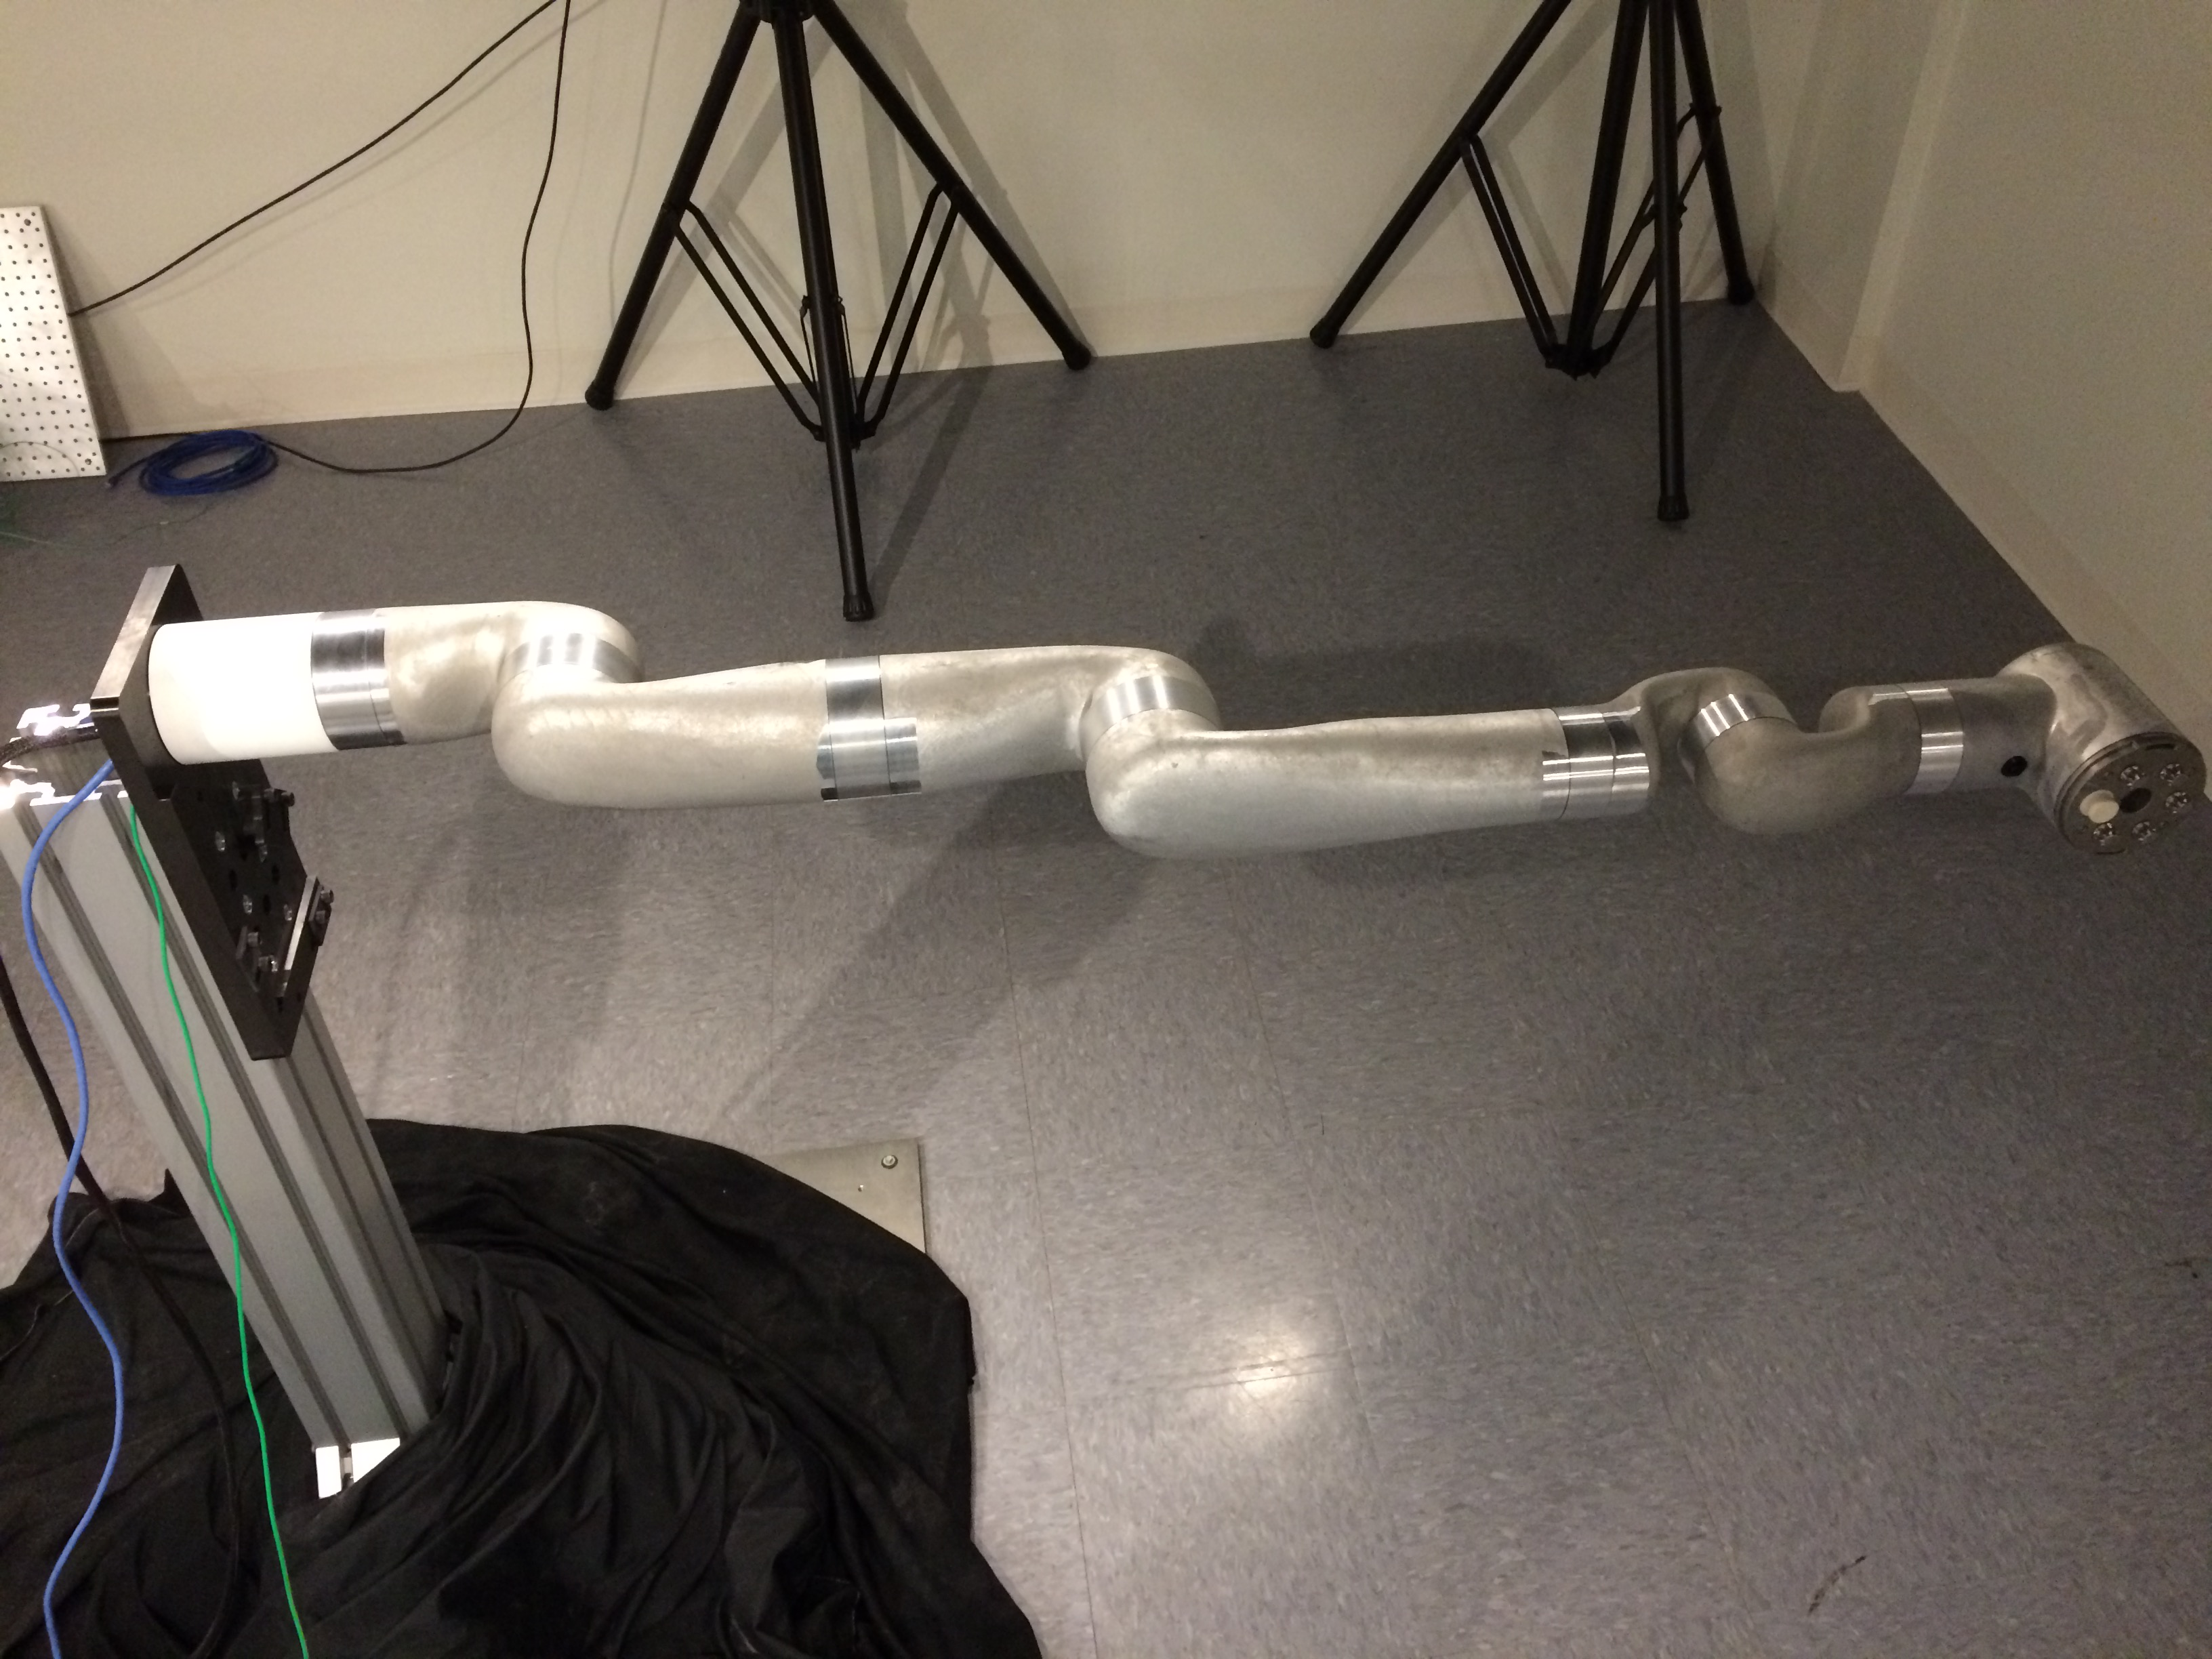
\includegraphics[width=0.9\textwidth]{./images/Pose12}
		\captionof{figure}{Pose12}
		\label{fig:pose12}
	\end{minipage}%
	\begin{minipage}{.5\textwidth}
		\centering
		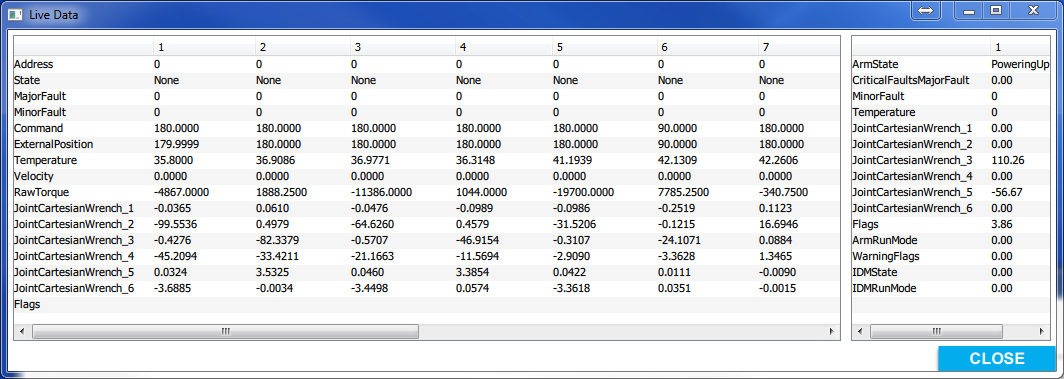
\includegraphics[width=0.9\textwidth]{./images/Pose13}
		\captionof{figure}{Pose13}
		\label{fig:pose13}
	\end{minipage}
\end{figure}

\begin{figure}
	\centering
	\begin{minipage}{.5\textwidth}
		\centering
		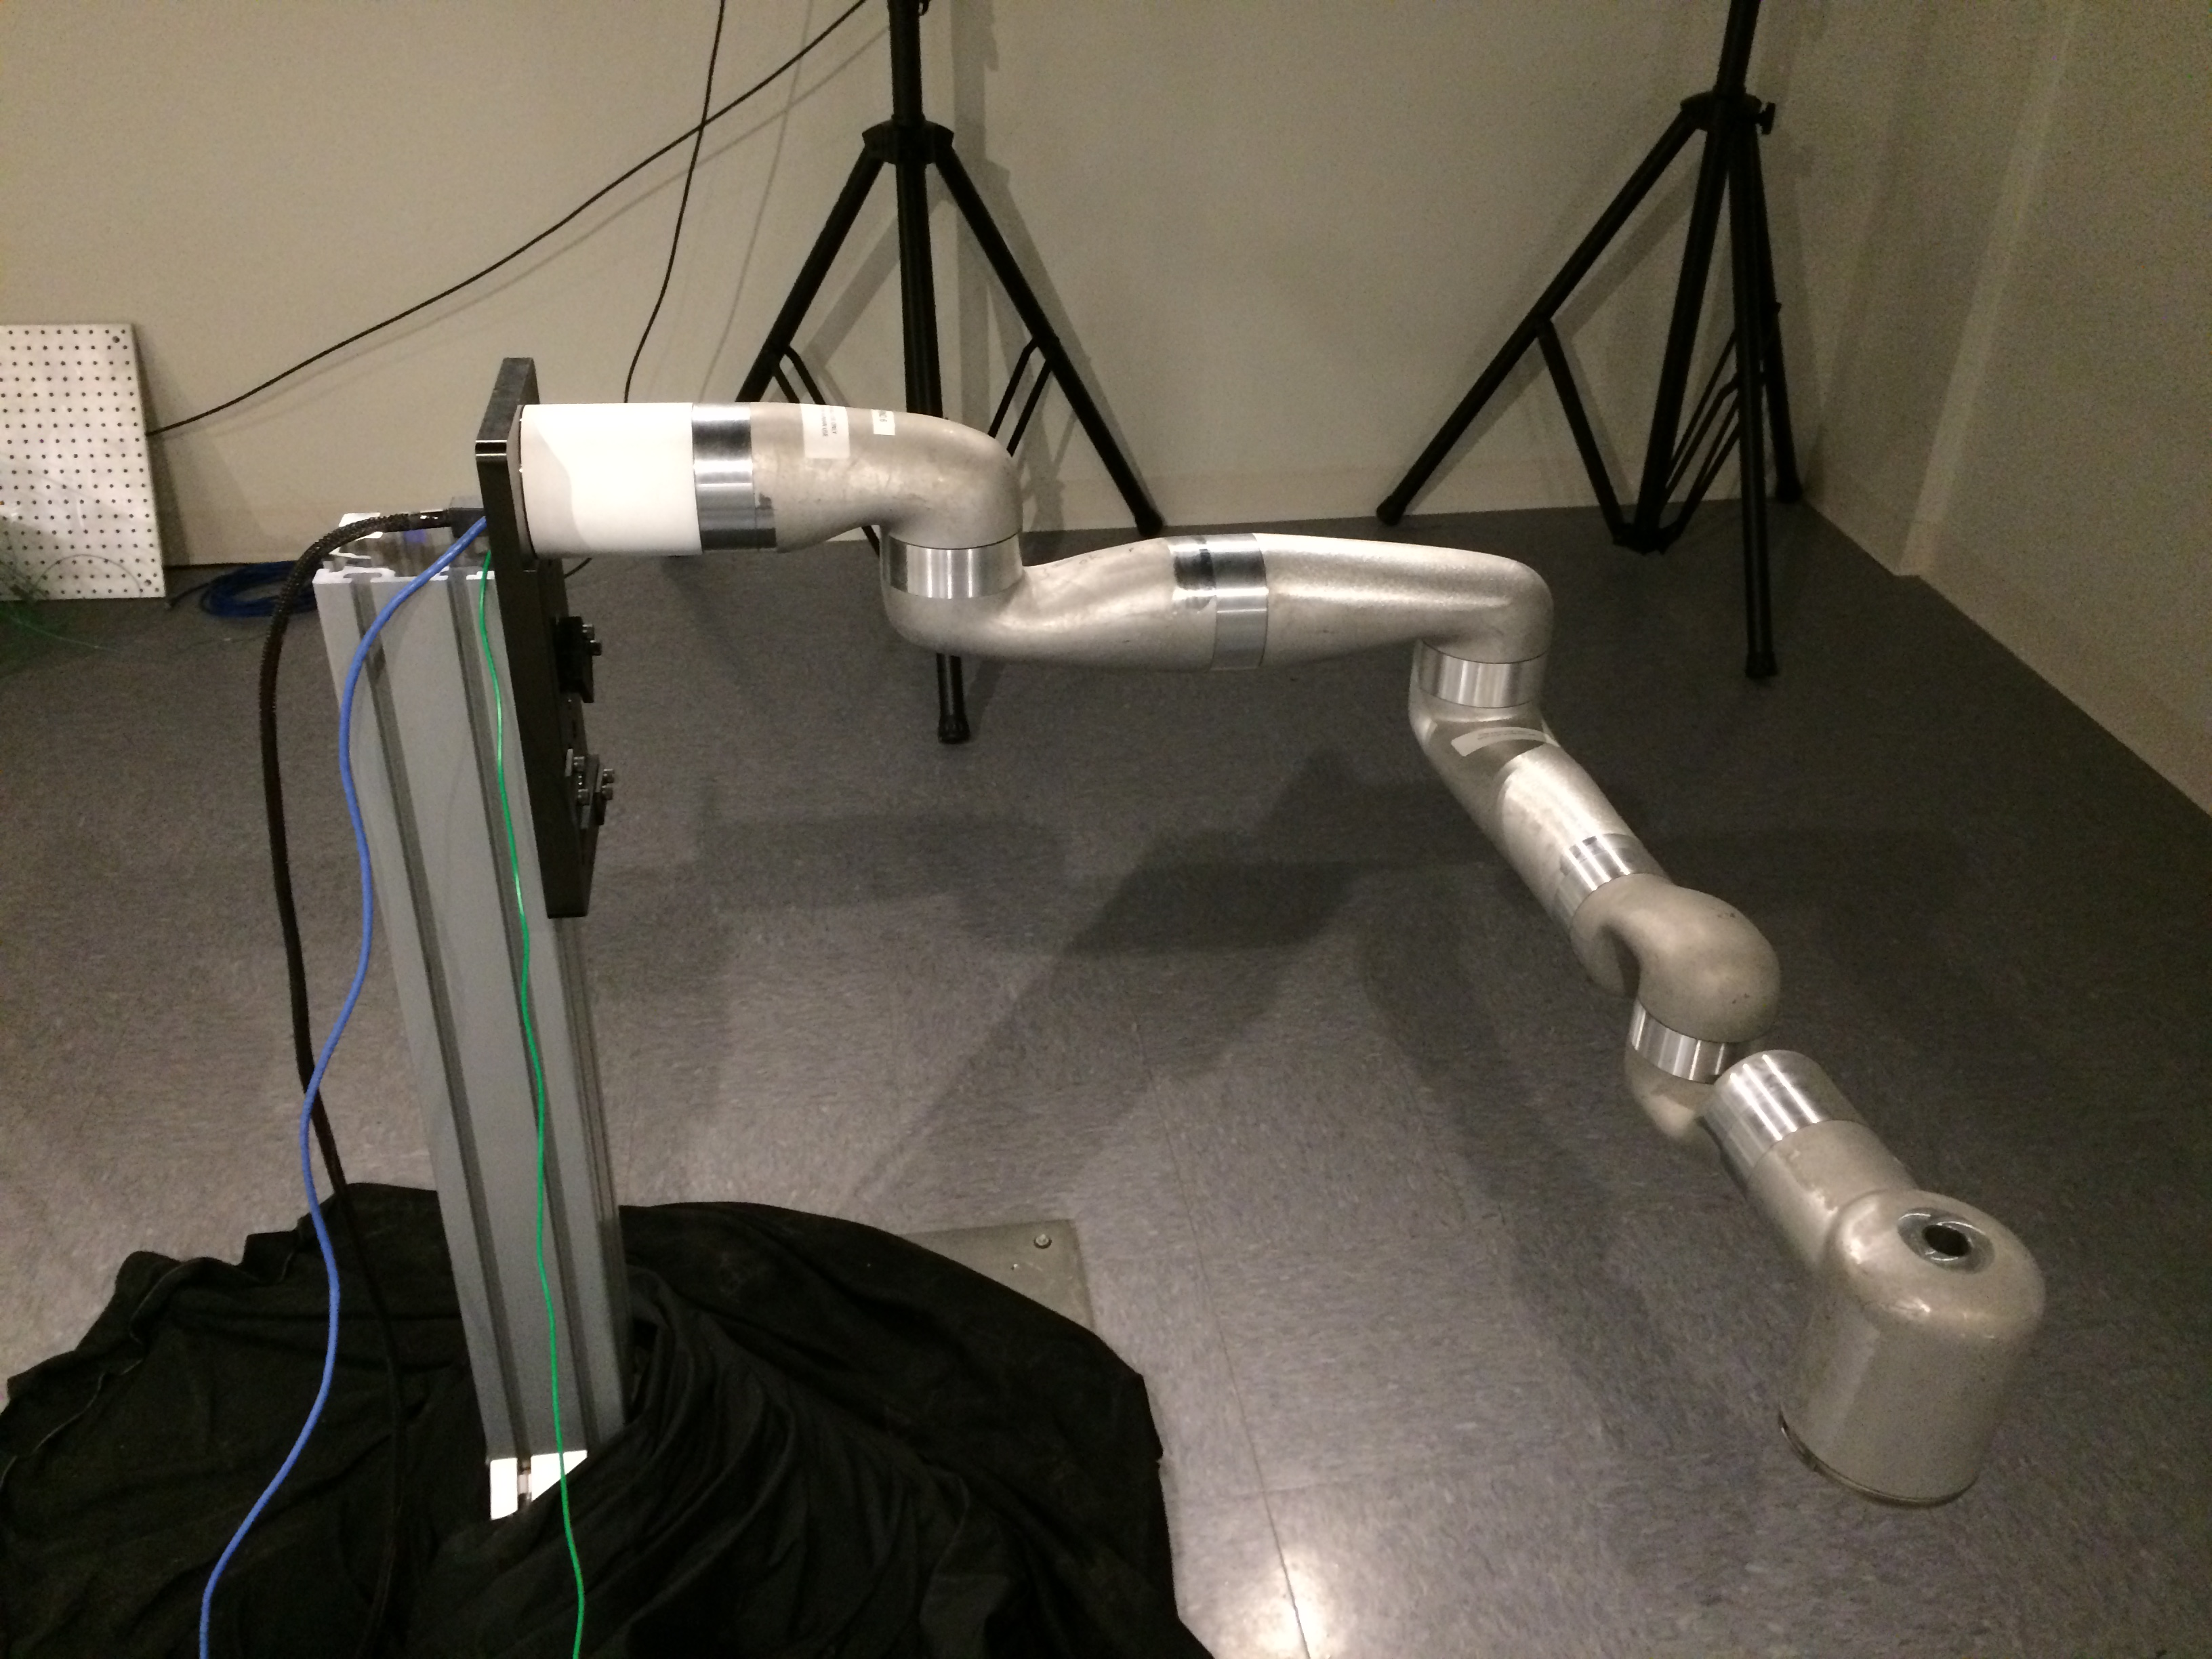
\includegraphics[width=0.9\textwidth]{./images/Pose14}
		\captionof{figure}{Pose14}
		\label{fig:pose14}
	\end{minipage}%
	\begin{minipage}{.5\textwidth}
		\centering
		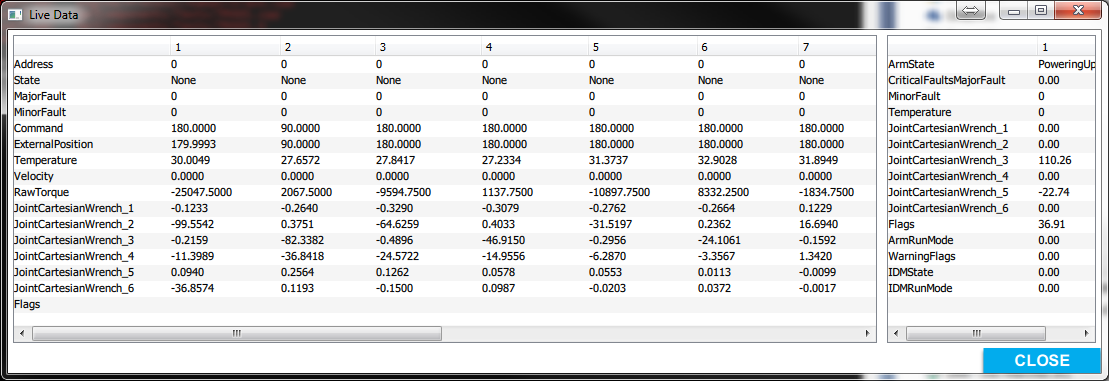
\includegraphics[width=0.9\textwidth]{./images/Pose15}
		\captionof{figure}{Pose15}
		\label{fig:pose15}
	\end{minipage}
\end{figure}





\newpage

\section{Test Procedure}
% testProcedure.tex
\subsection{Source Code Repository}
PR37 MS7 arm uses a different architecture than MS5/6 arm. The branch of each repository is listed below:
\begin{itemize}
	\item keos: release/1.8
	\item bitwin: development (commit ID: 971e7b7, small changes on feature/SWPreleaseKit3\_CTRL\_Update)
	\item rtcontrol\_nextgen: feature/UpdateControlCOnfigFunction
	\item sdk\_assitive: feature/SWPrelease\_CTRL\_Update
\end{itemize}

\subsection{Data acquisition}
\begin{enumerate}
	\item run executable rtcontrol on QNX
	\item run sdk\_assitive to get NOVA interface on PC (as in Figure \ref{fig:nova})
	\item select AURIS in NOVA
	\item select AURIS Control in NOVA
	\item set IP of QNX, Run Mode in "run", and then click Connect
	\item release robot break
	\item input a pre-defined robot configuration in Custom Configuration in NOVA and send it to robot
	\item click Live Data to view data in real time
	\item make a screenshot of Live Data to collect data
	\item input a new pre-defined robot configuration and repeat the steps to get data for all pre-defined robot configurations
\end{enumerate}

\begin{figure}
	\begin{center}
		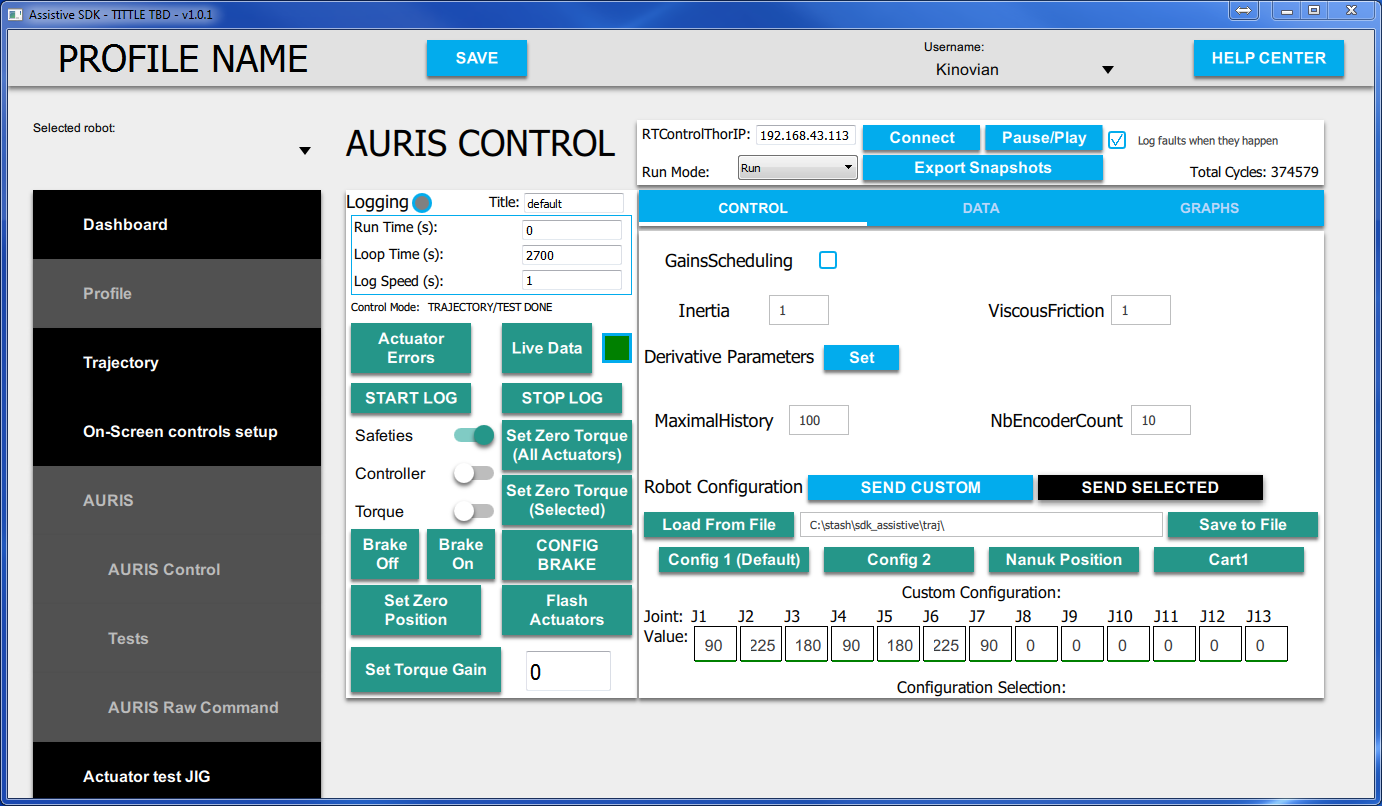
\includegraphics[width=0.9\textwidth]{./images/NOVA}%
		\caption{NOVA interface}
		\label{fig:nova}%
	\end{center}
\end{figure}


\newpage

\section{Test Results}
% Draft of the tests results

With the predefined poses in Table \ref{table-groupA} and Table \ref{table-groupB}, we obtained the computed JointWrench\_PC. The JointWrech\_Base is obtained while sending the same joint position command, as described in Section \ref{sec:testProcedure}. The $i^{th}$ joint wrench contains force and torque along x, y and z axis of $i^{th}$ joint frame. The difference of these two joint wrench values are defined as abs(JointWrench\_PC - JointWrech\_Base). 

\begin{figure}[H]
	\begin{center}
		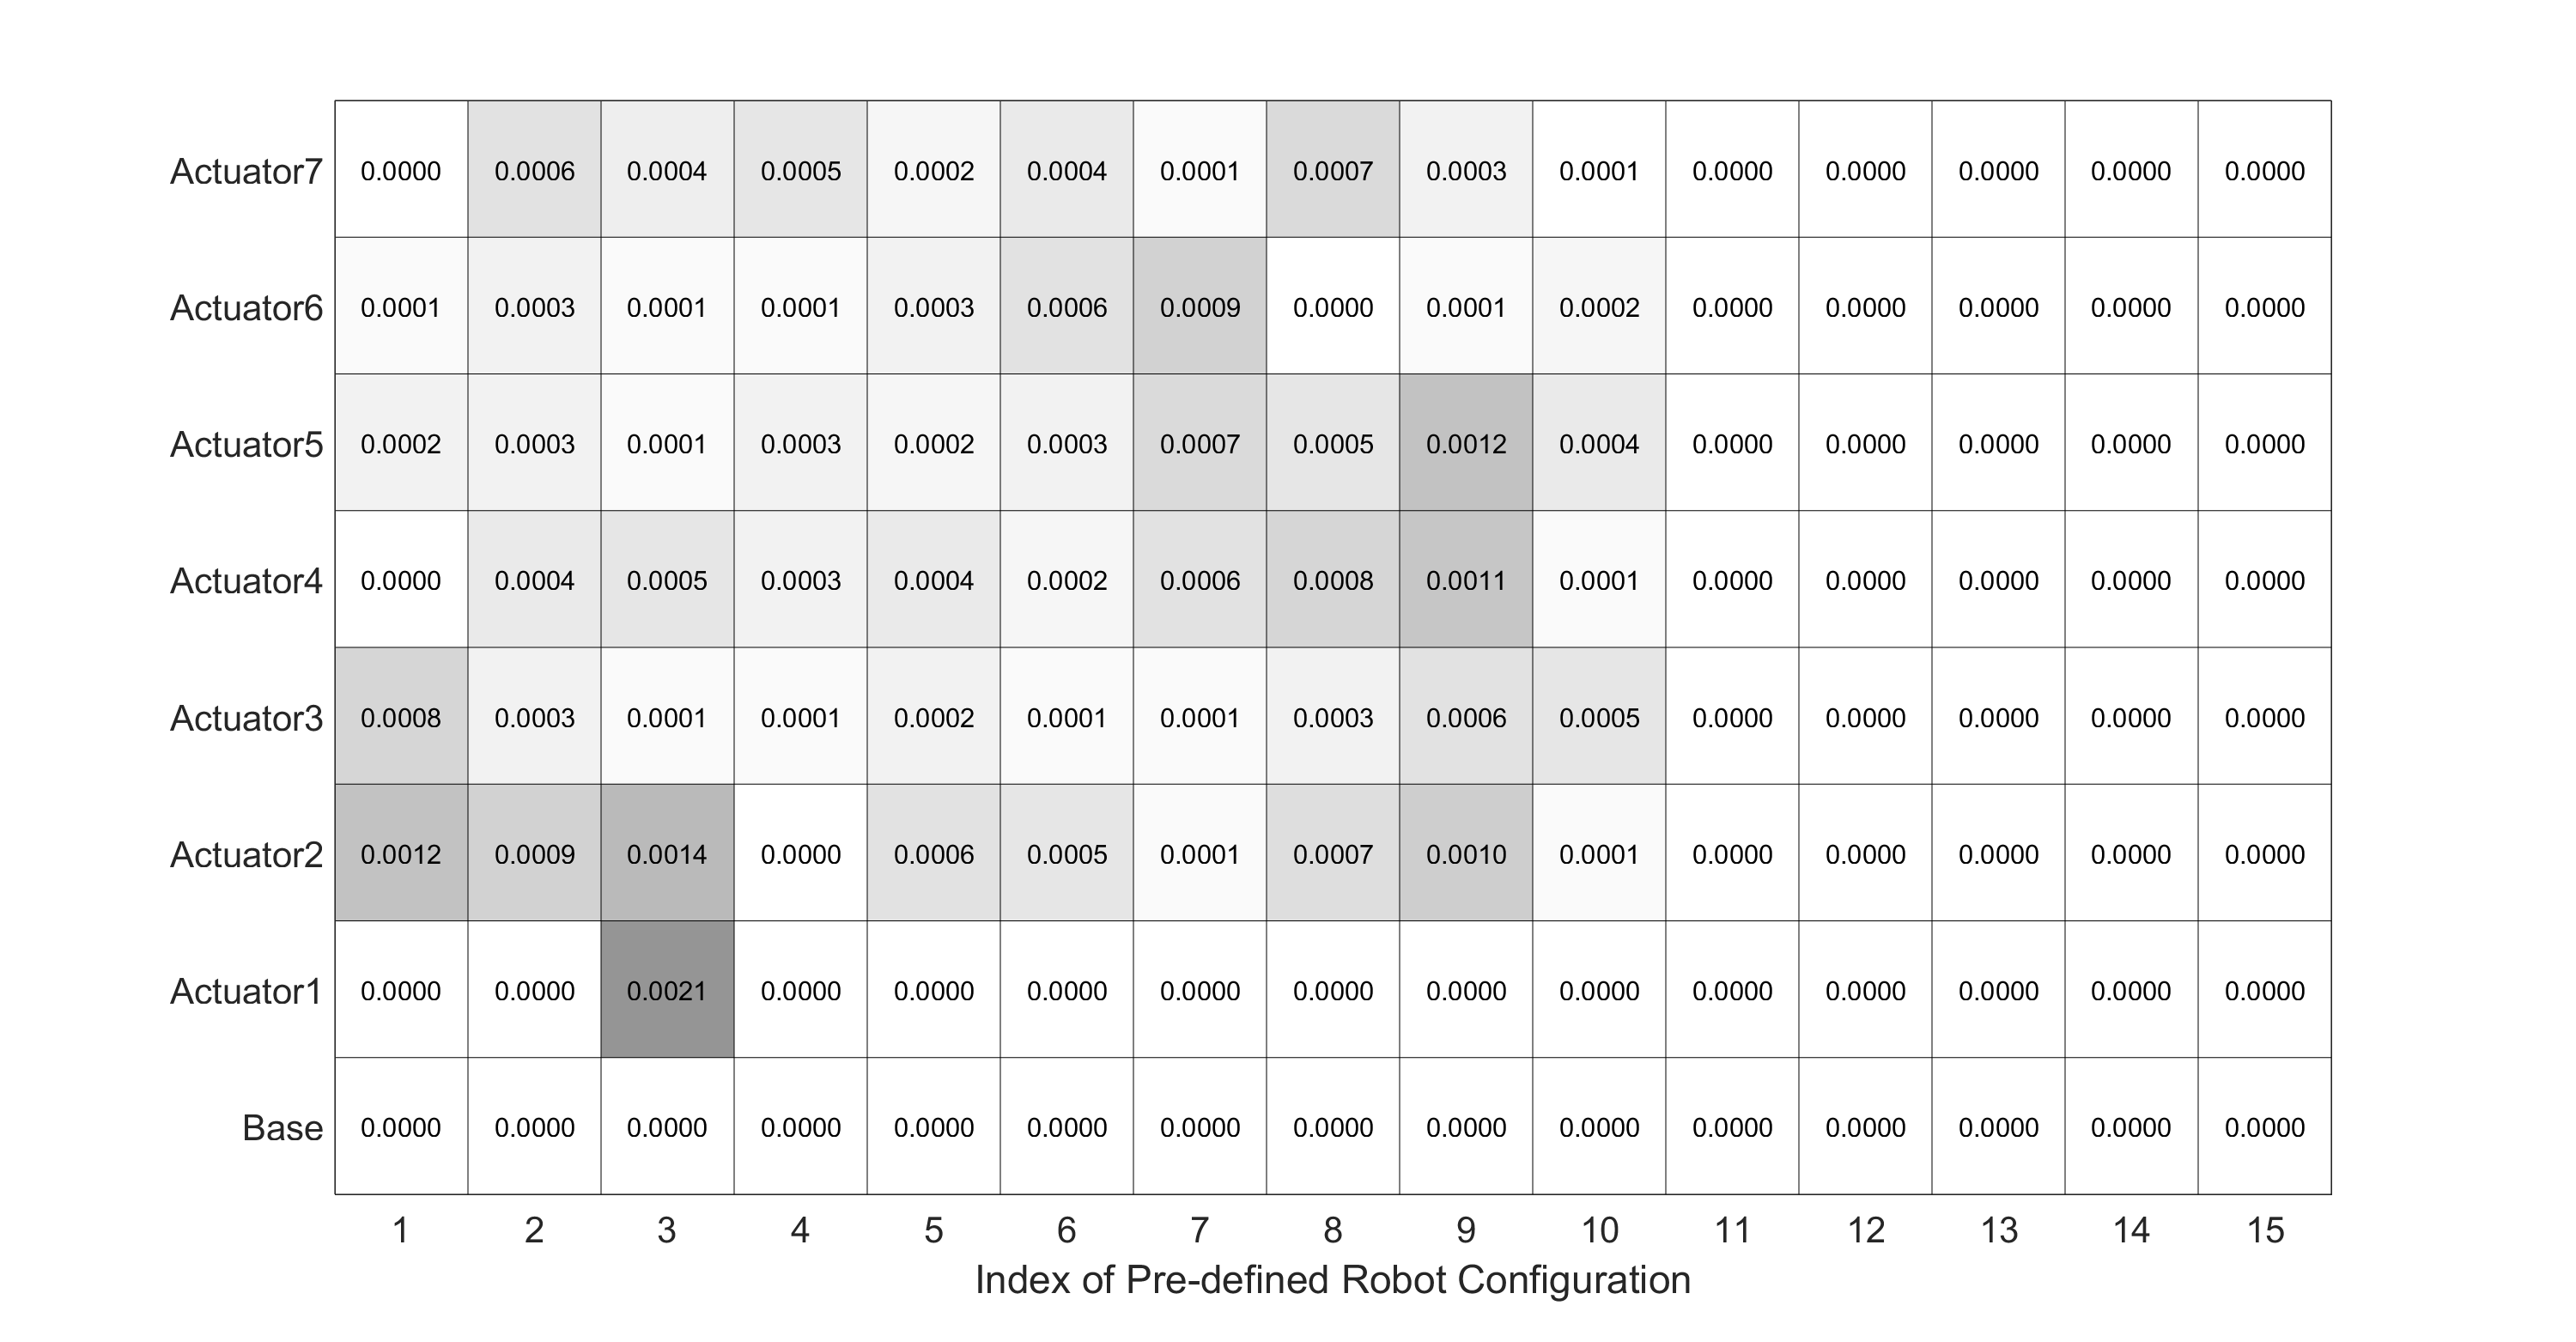
\includegraphics[width=0.9\textwidth]{./images/ForceXError.png}%
		\caption{Error of Force along X axis in N}
		\label{fig:ForceXError}%
	\end{center}
\end{figure}

\begin{figure}[H]
	\begin{center}
		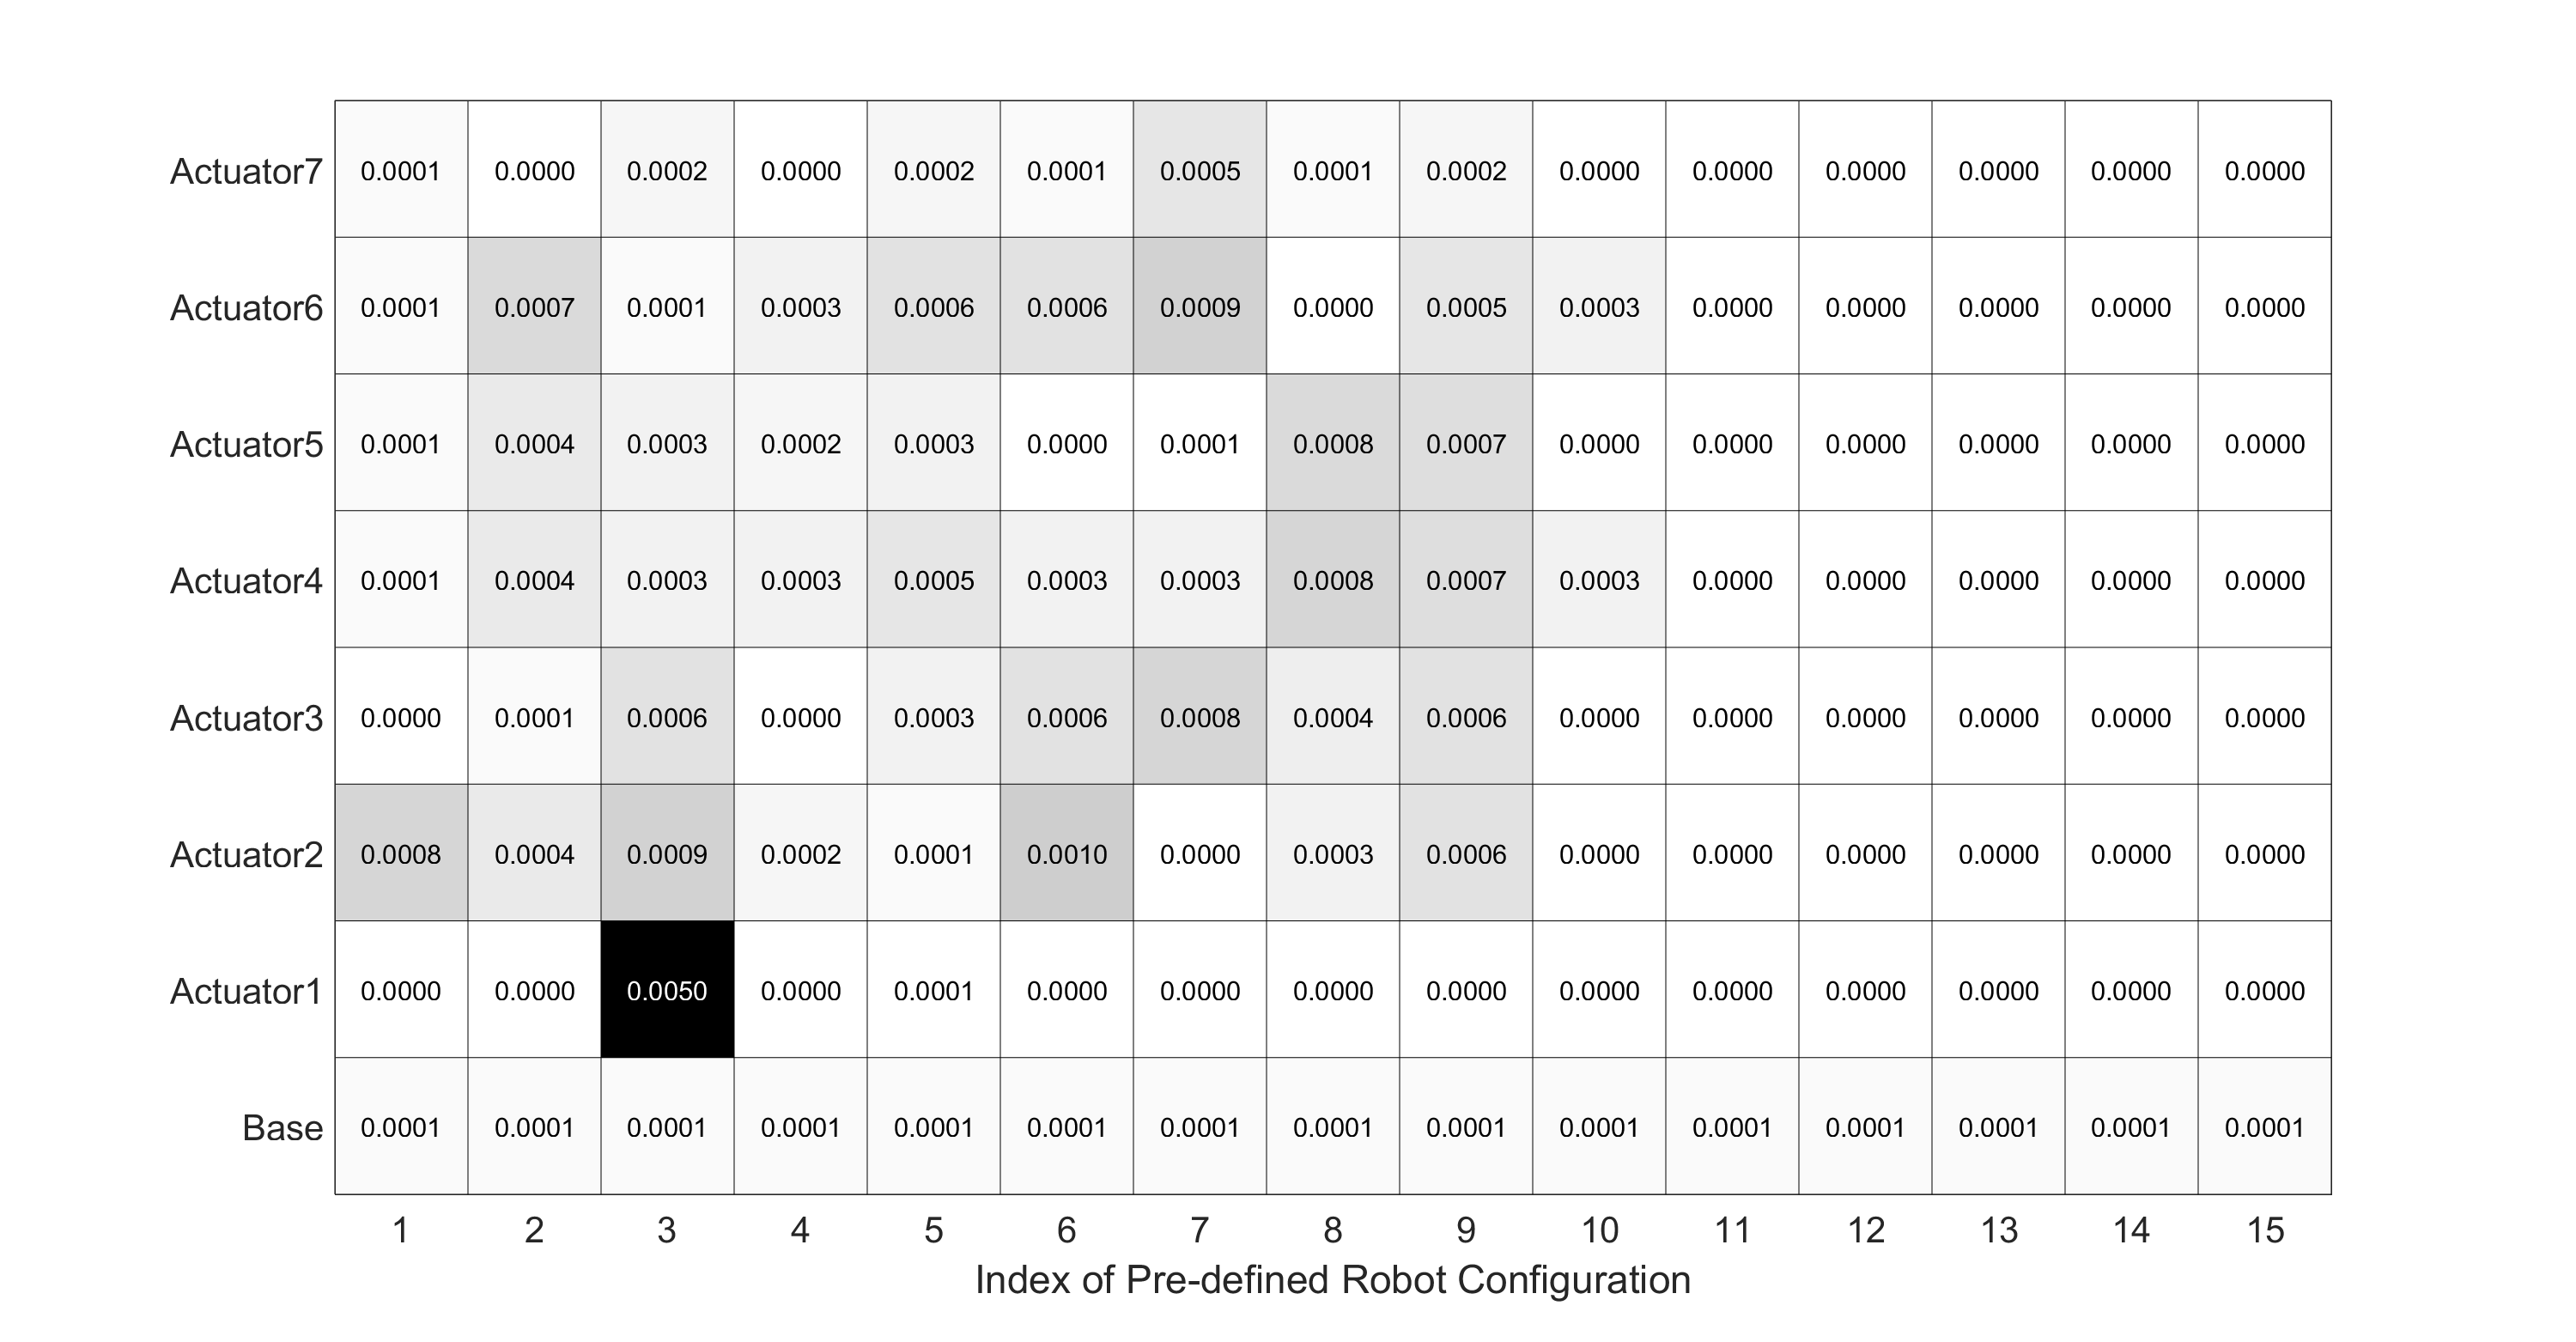
\includegraphics[width=0.9\textwidth]{./images/ForceYError.png}%
		\caption{Error of Force along Y axis in N}
		\label{fig:ForceYError}%
	\end{center}
\end{figure}

\begin{figure}[H]
	\begin{center}
		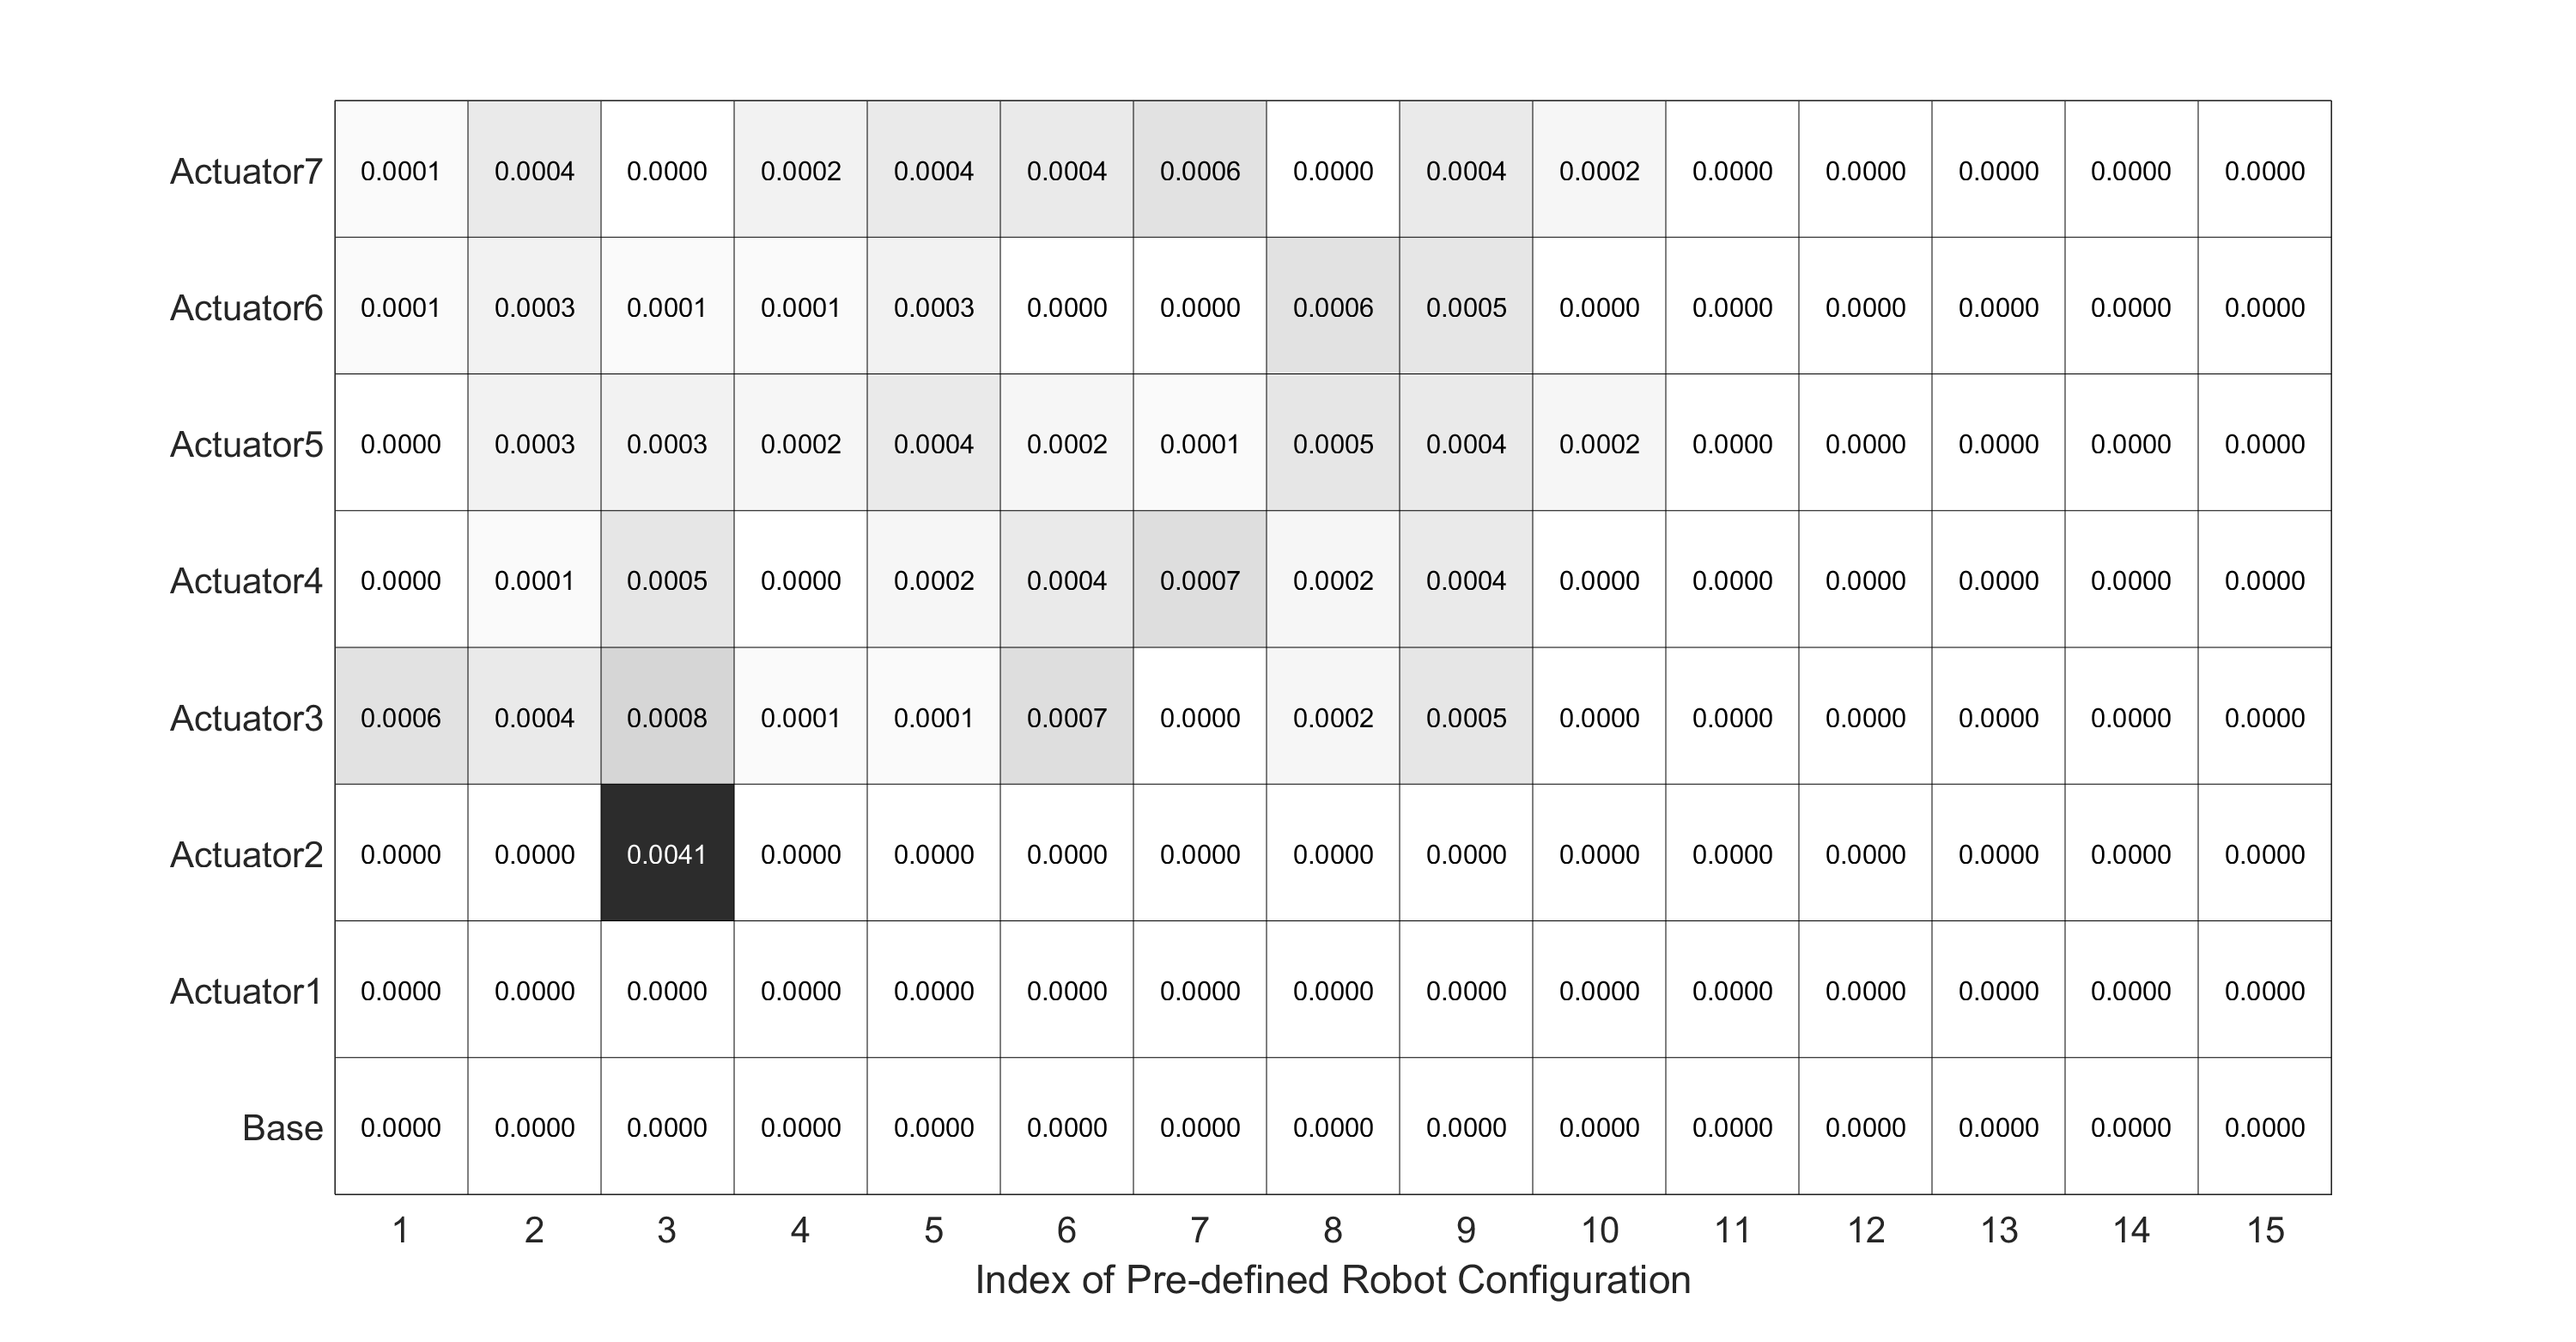
\includegraphics[width=0.9\textwidth]{./images/ForceZError.png}%
		\caption{Error of Force along Z axis in N}
		\label{fig:ForceZError}%
	\end{center}
\end{figure}

\begin{figure}[H]
	\begin{center}
		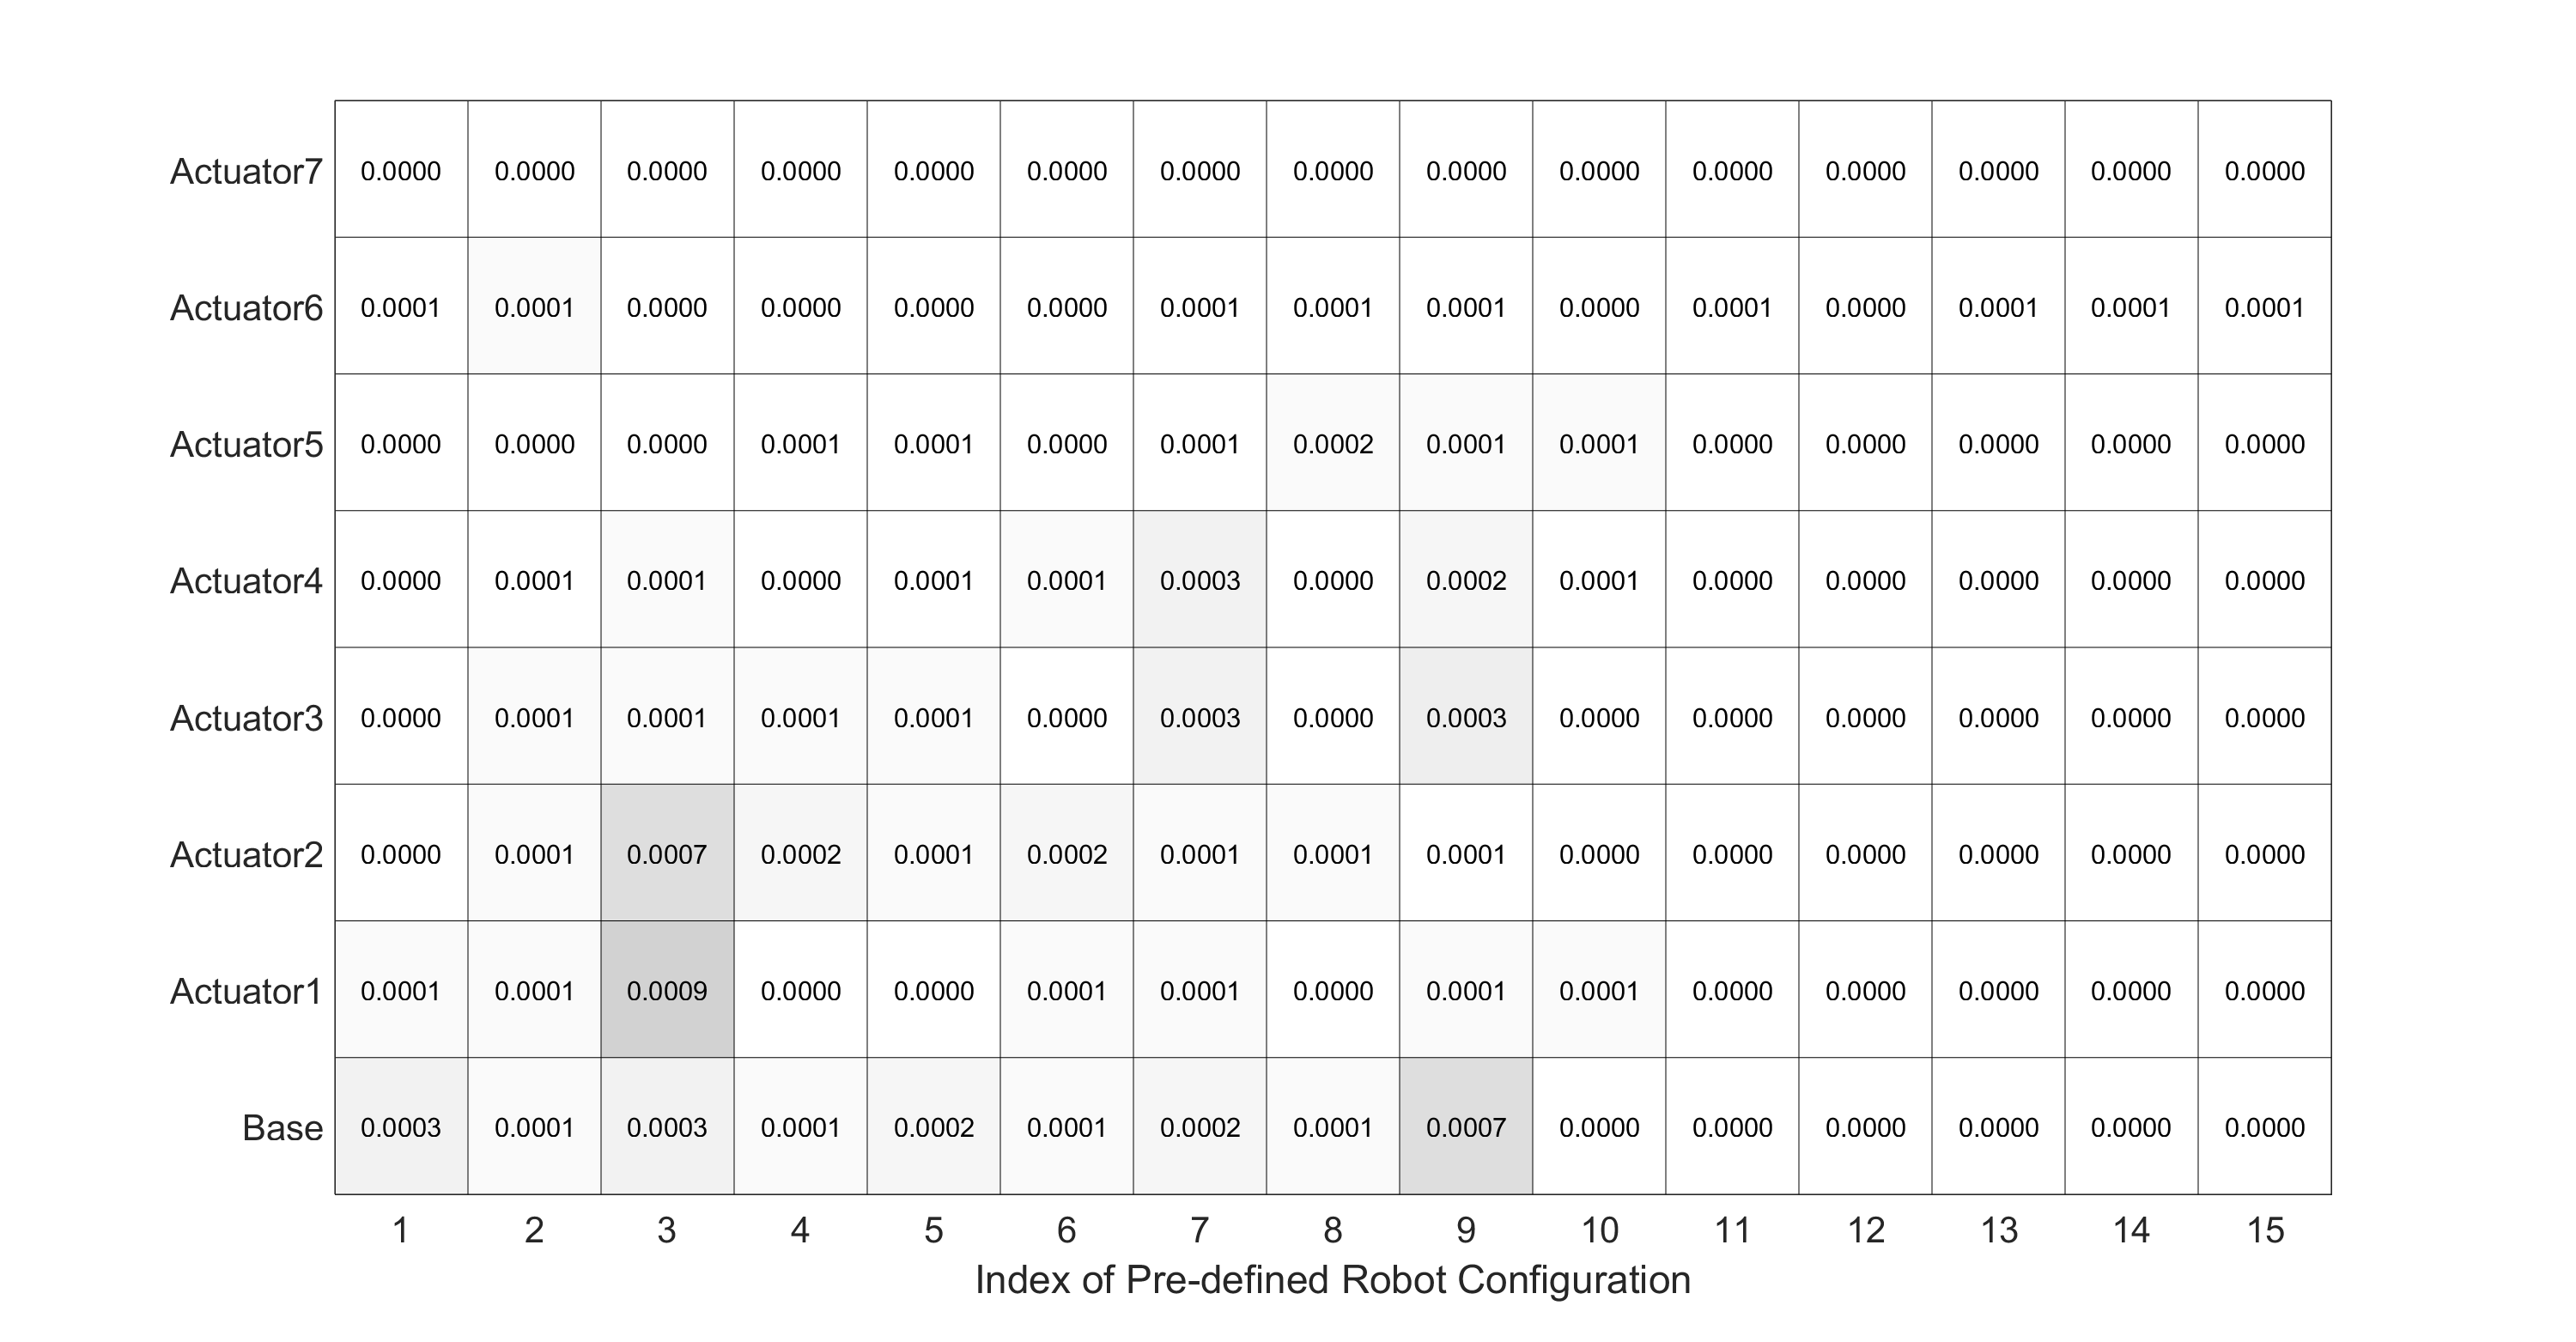
\includegraphics[width=0.9\textwidth]{./images/TorqueXError.png}%
		\caption{Error of Torque along X axis in Nm}
		\label{fig:TorqueXError}%
	\end{center}
\end{figure}

\begin{figure}[H]
	\begin{center}
		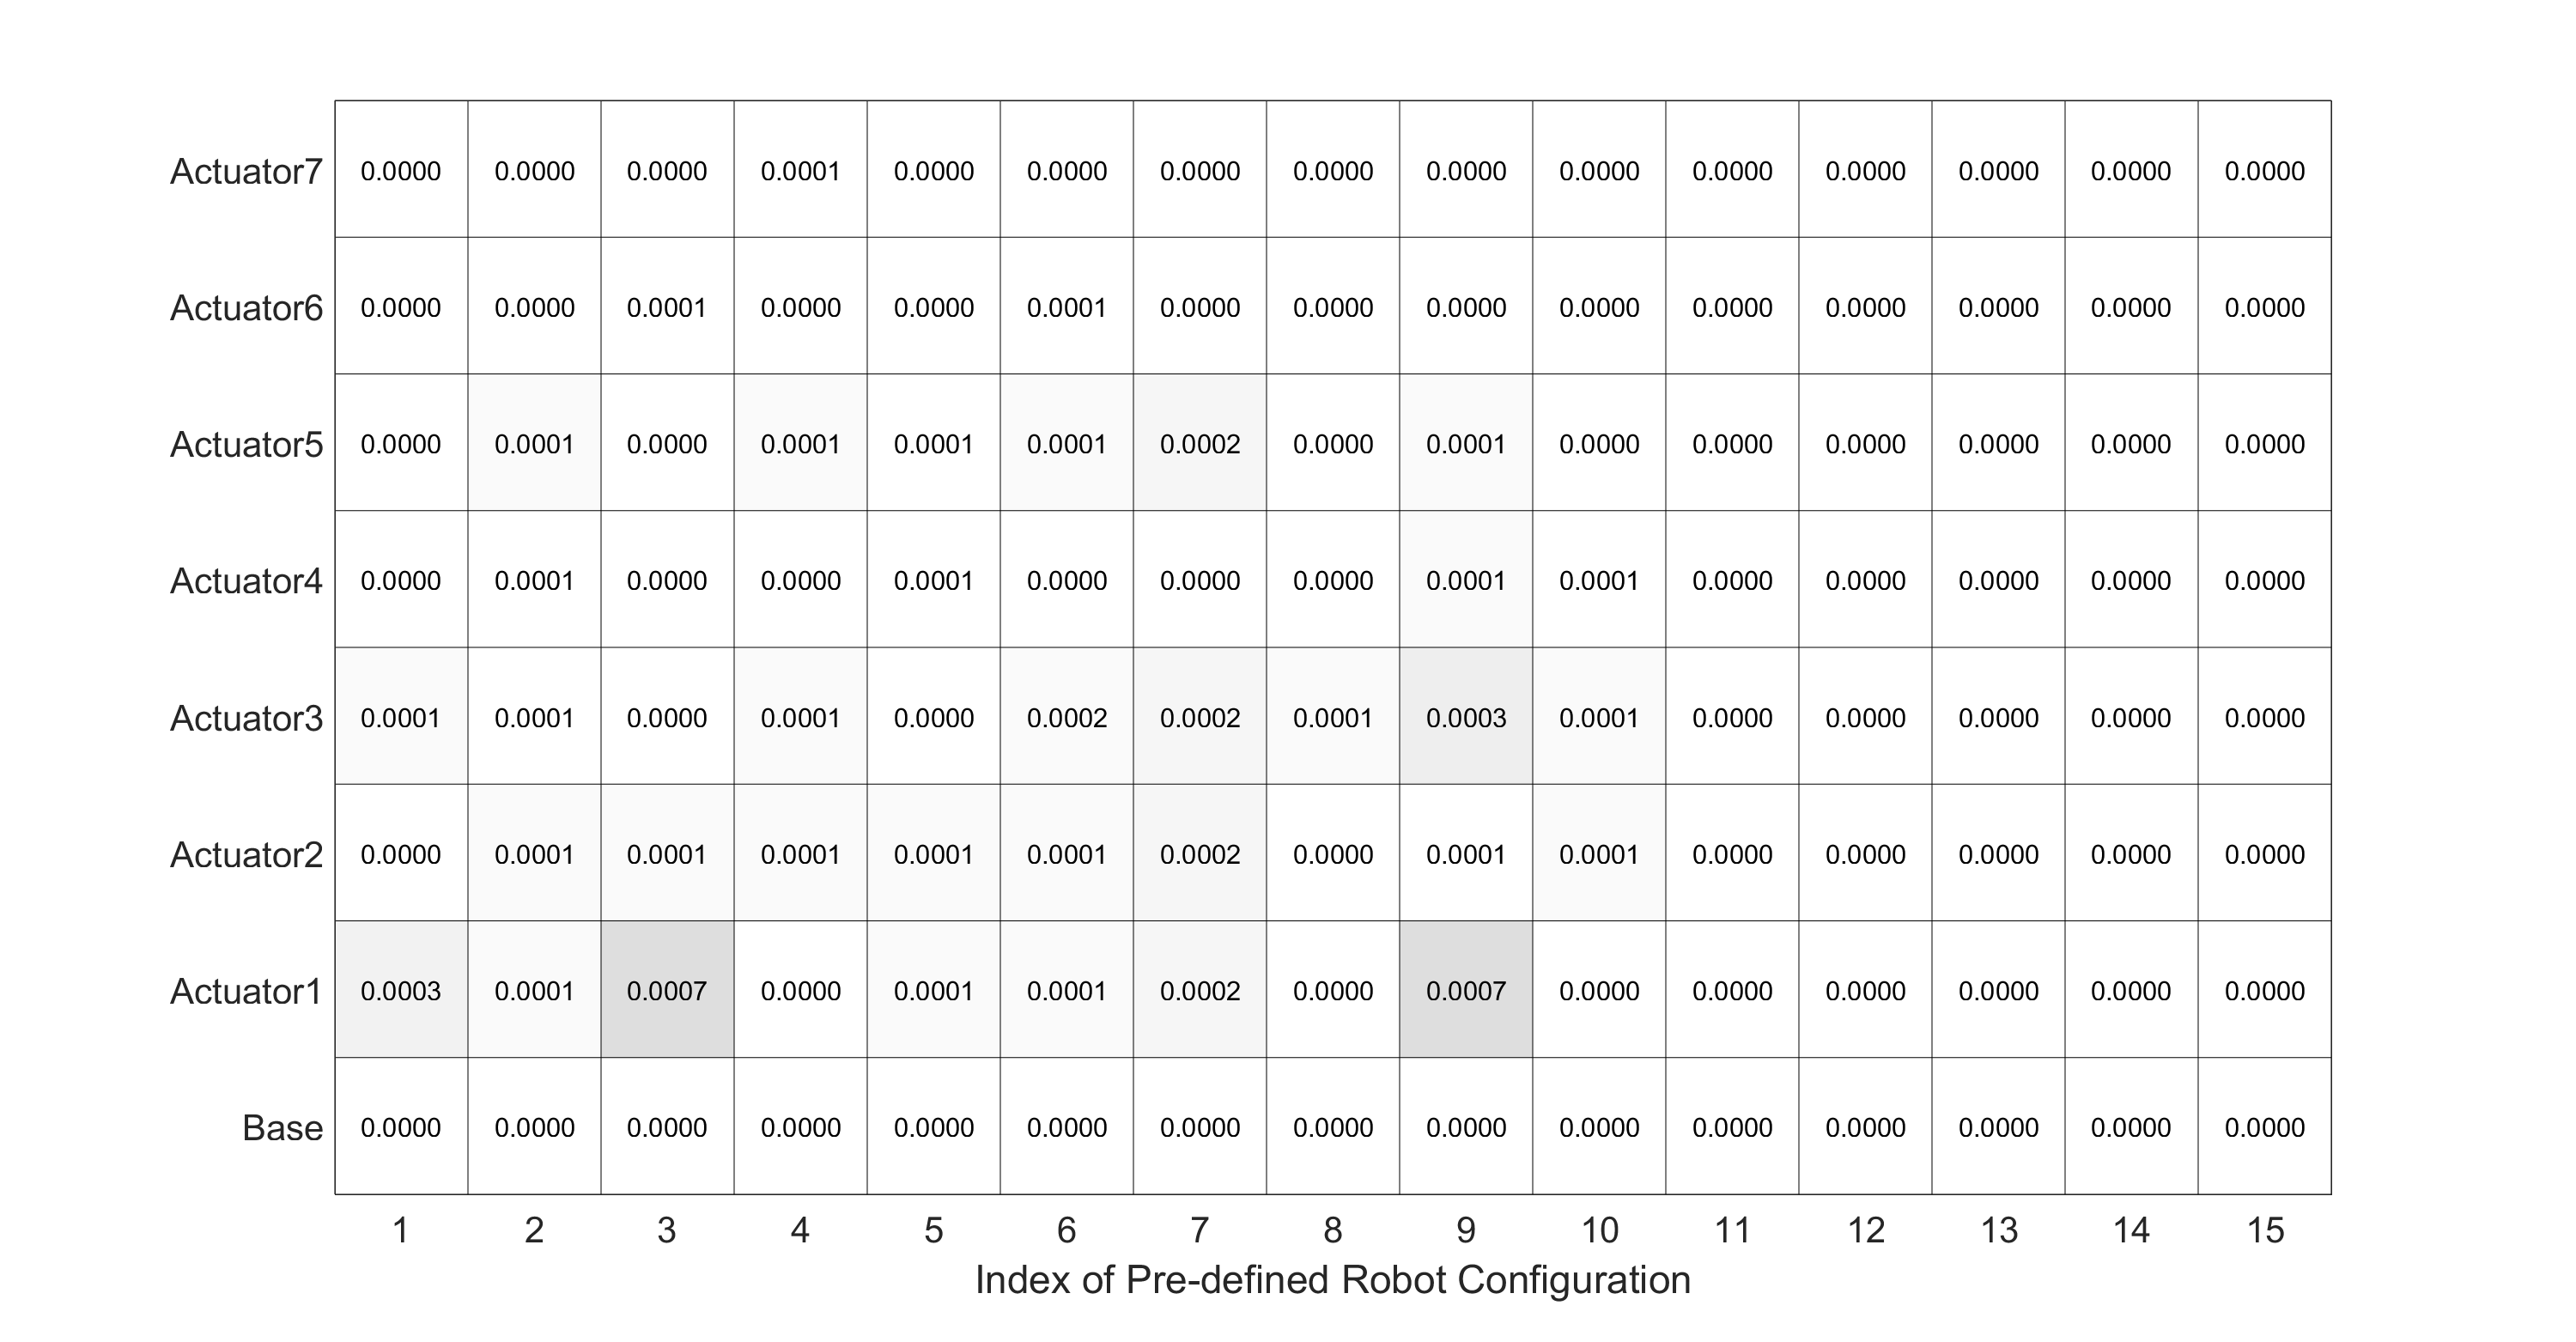
\includegraphics[width=0.9\textwidth]{./images/TorqueYError.png}%
		\caption{Error of Torque along Y axis in Nm}
		\label{fig:TorqueYError}%
	\end{center}
\end{figure}

\begin{figure}[H]
	\begin{center}
		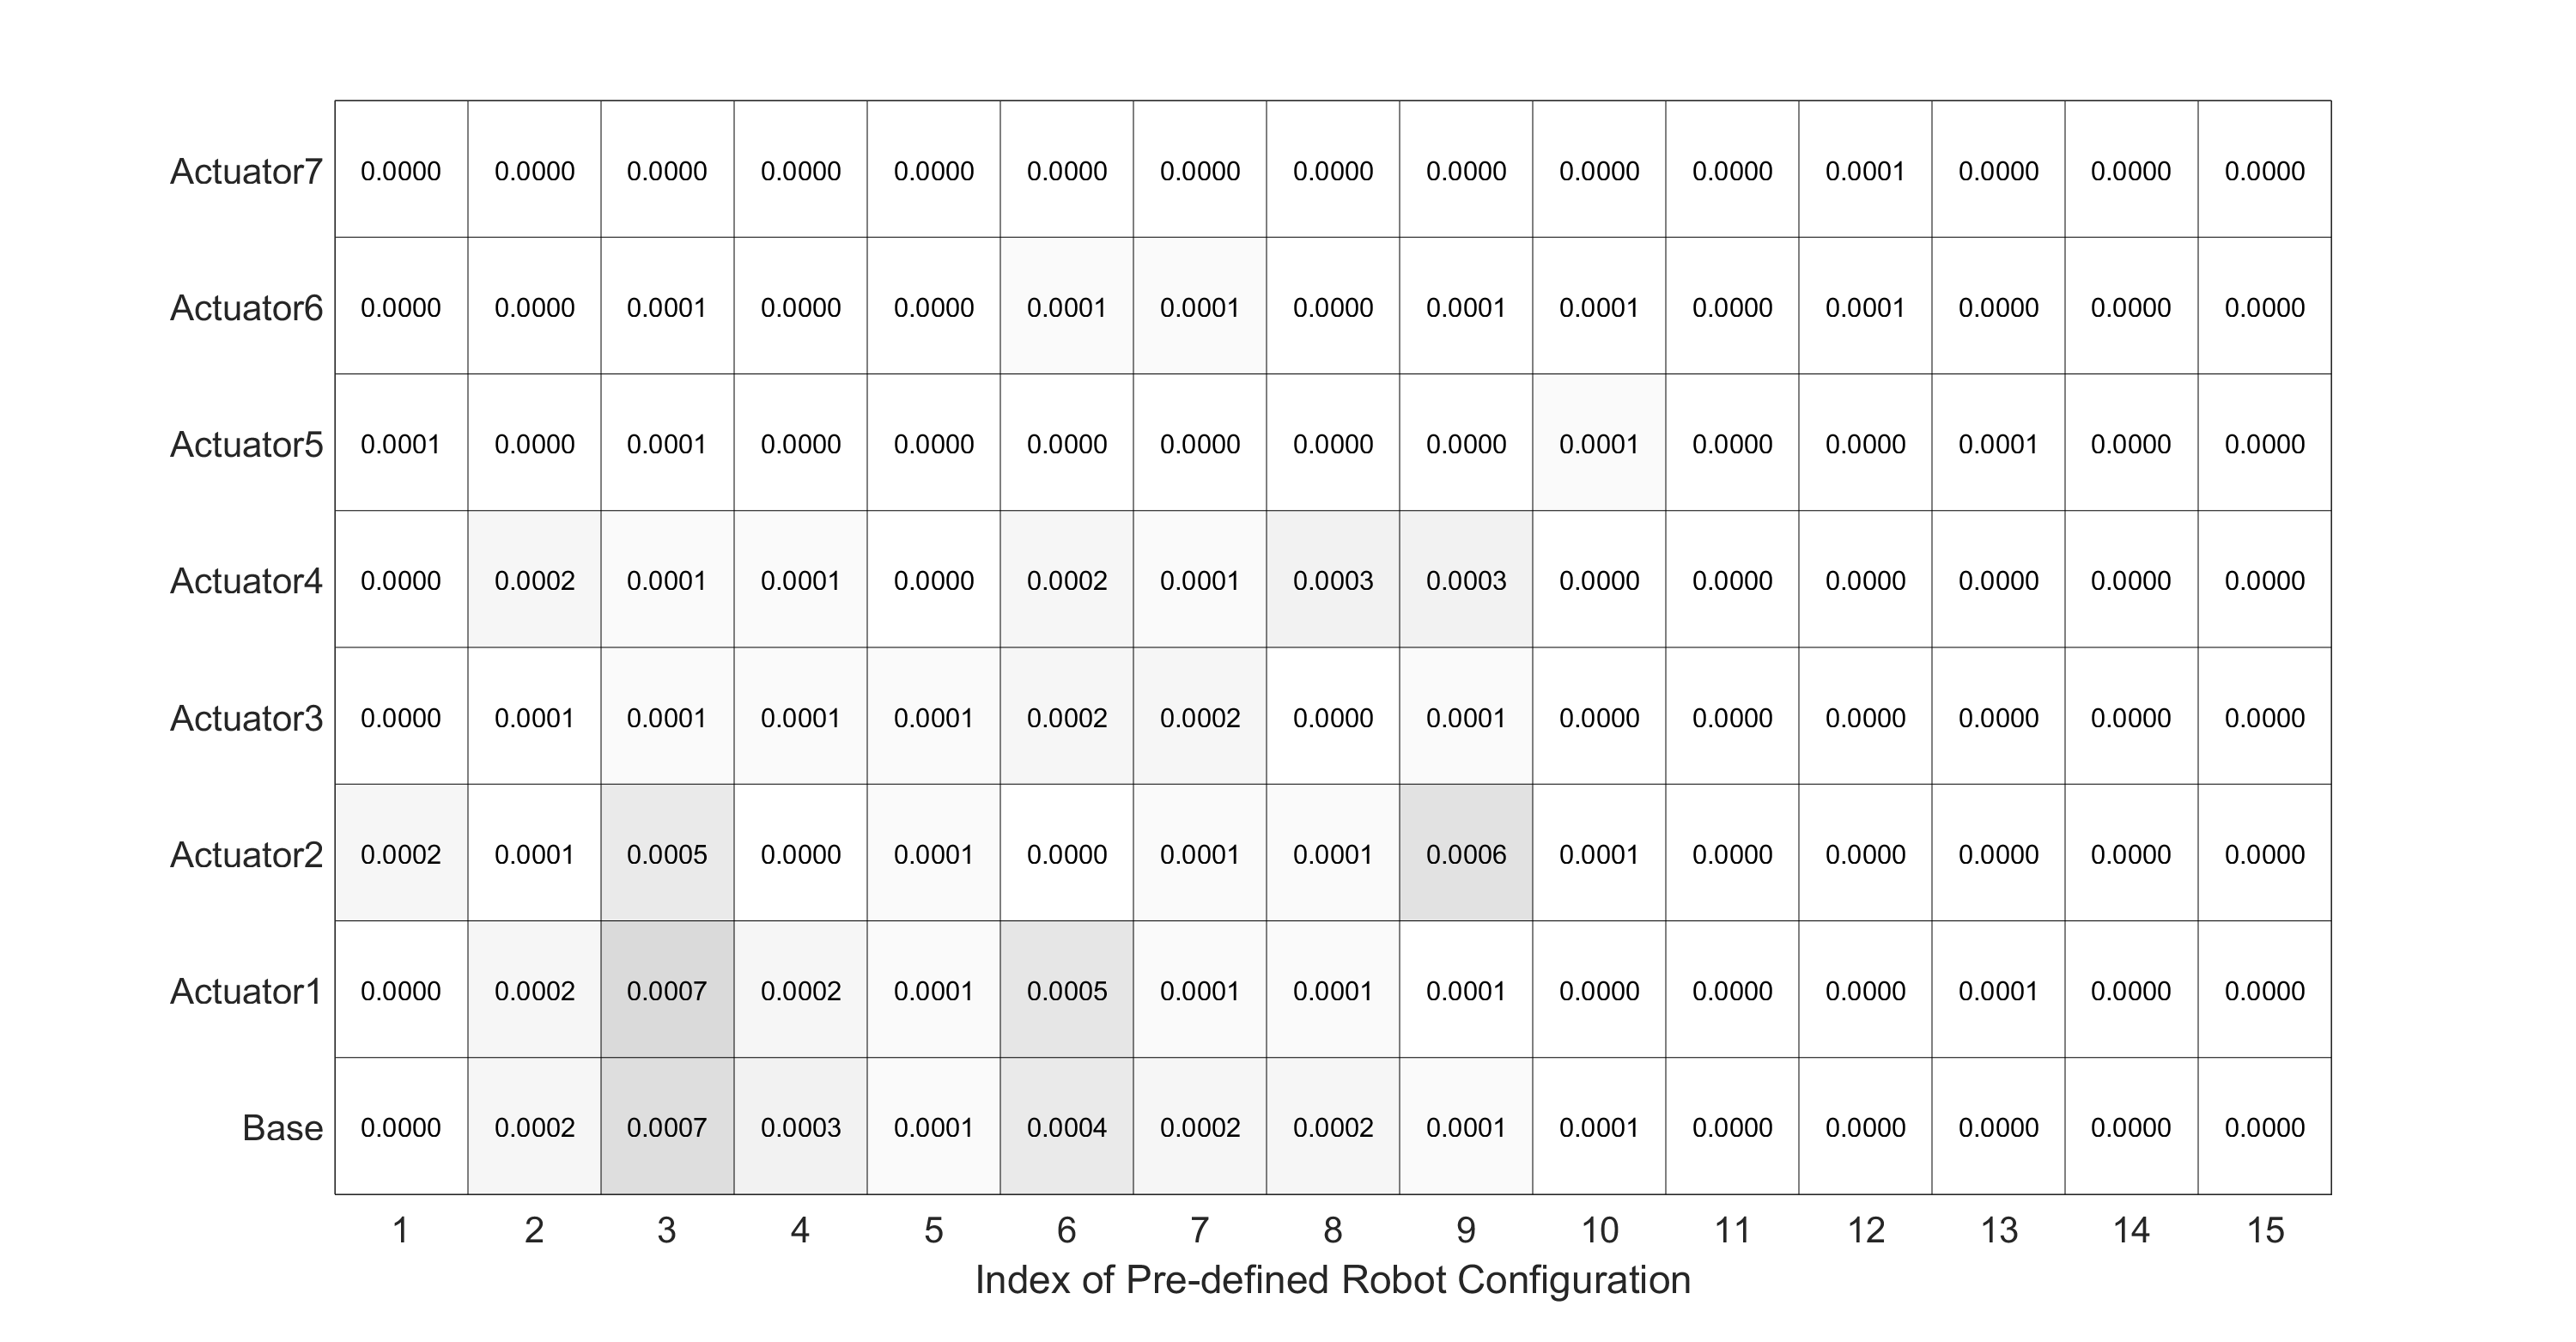
\includegraphics[width=0.9\textwidth]{./images/TorqueZError.png}%
		\caption{Error of Torque along Z axis in Nm}
		\label{fig:TorqueZError}%
	\end{center}
\end{figure}

The Figure \ref{fig:ForceXError} to Figure \ref{fig:TorqueZError} shows the error distribution of all the tests in 15 poses (horizontal axis). The vertical axis indicates the joint index, with base with index 1 and joint 7 with index 8. The color of each cell demonstrates the error of the corresponding test (the darker, the worse). In worst cases, the error of joint force reach 0.005N and torque is around 0.001Nm. 

It is noticed that the robot cannot perfectly reach the predefined configurations. It is more meaningful to compute JointWrench\_PC based on robot joint position feedback for the comparison, as shown in Figure \ref{fig:ForceXErrorFB}to Figure \ref{fig:TorqueZErrorFB}. It is obvious that differences are ten times smaller, in the scale of $10^{-4}$ N (Force) or Nm(Torque). This difference may due to the provided data precision in the code or computation round up. 


\begin{figure}[H]
	\begin{center}
		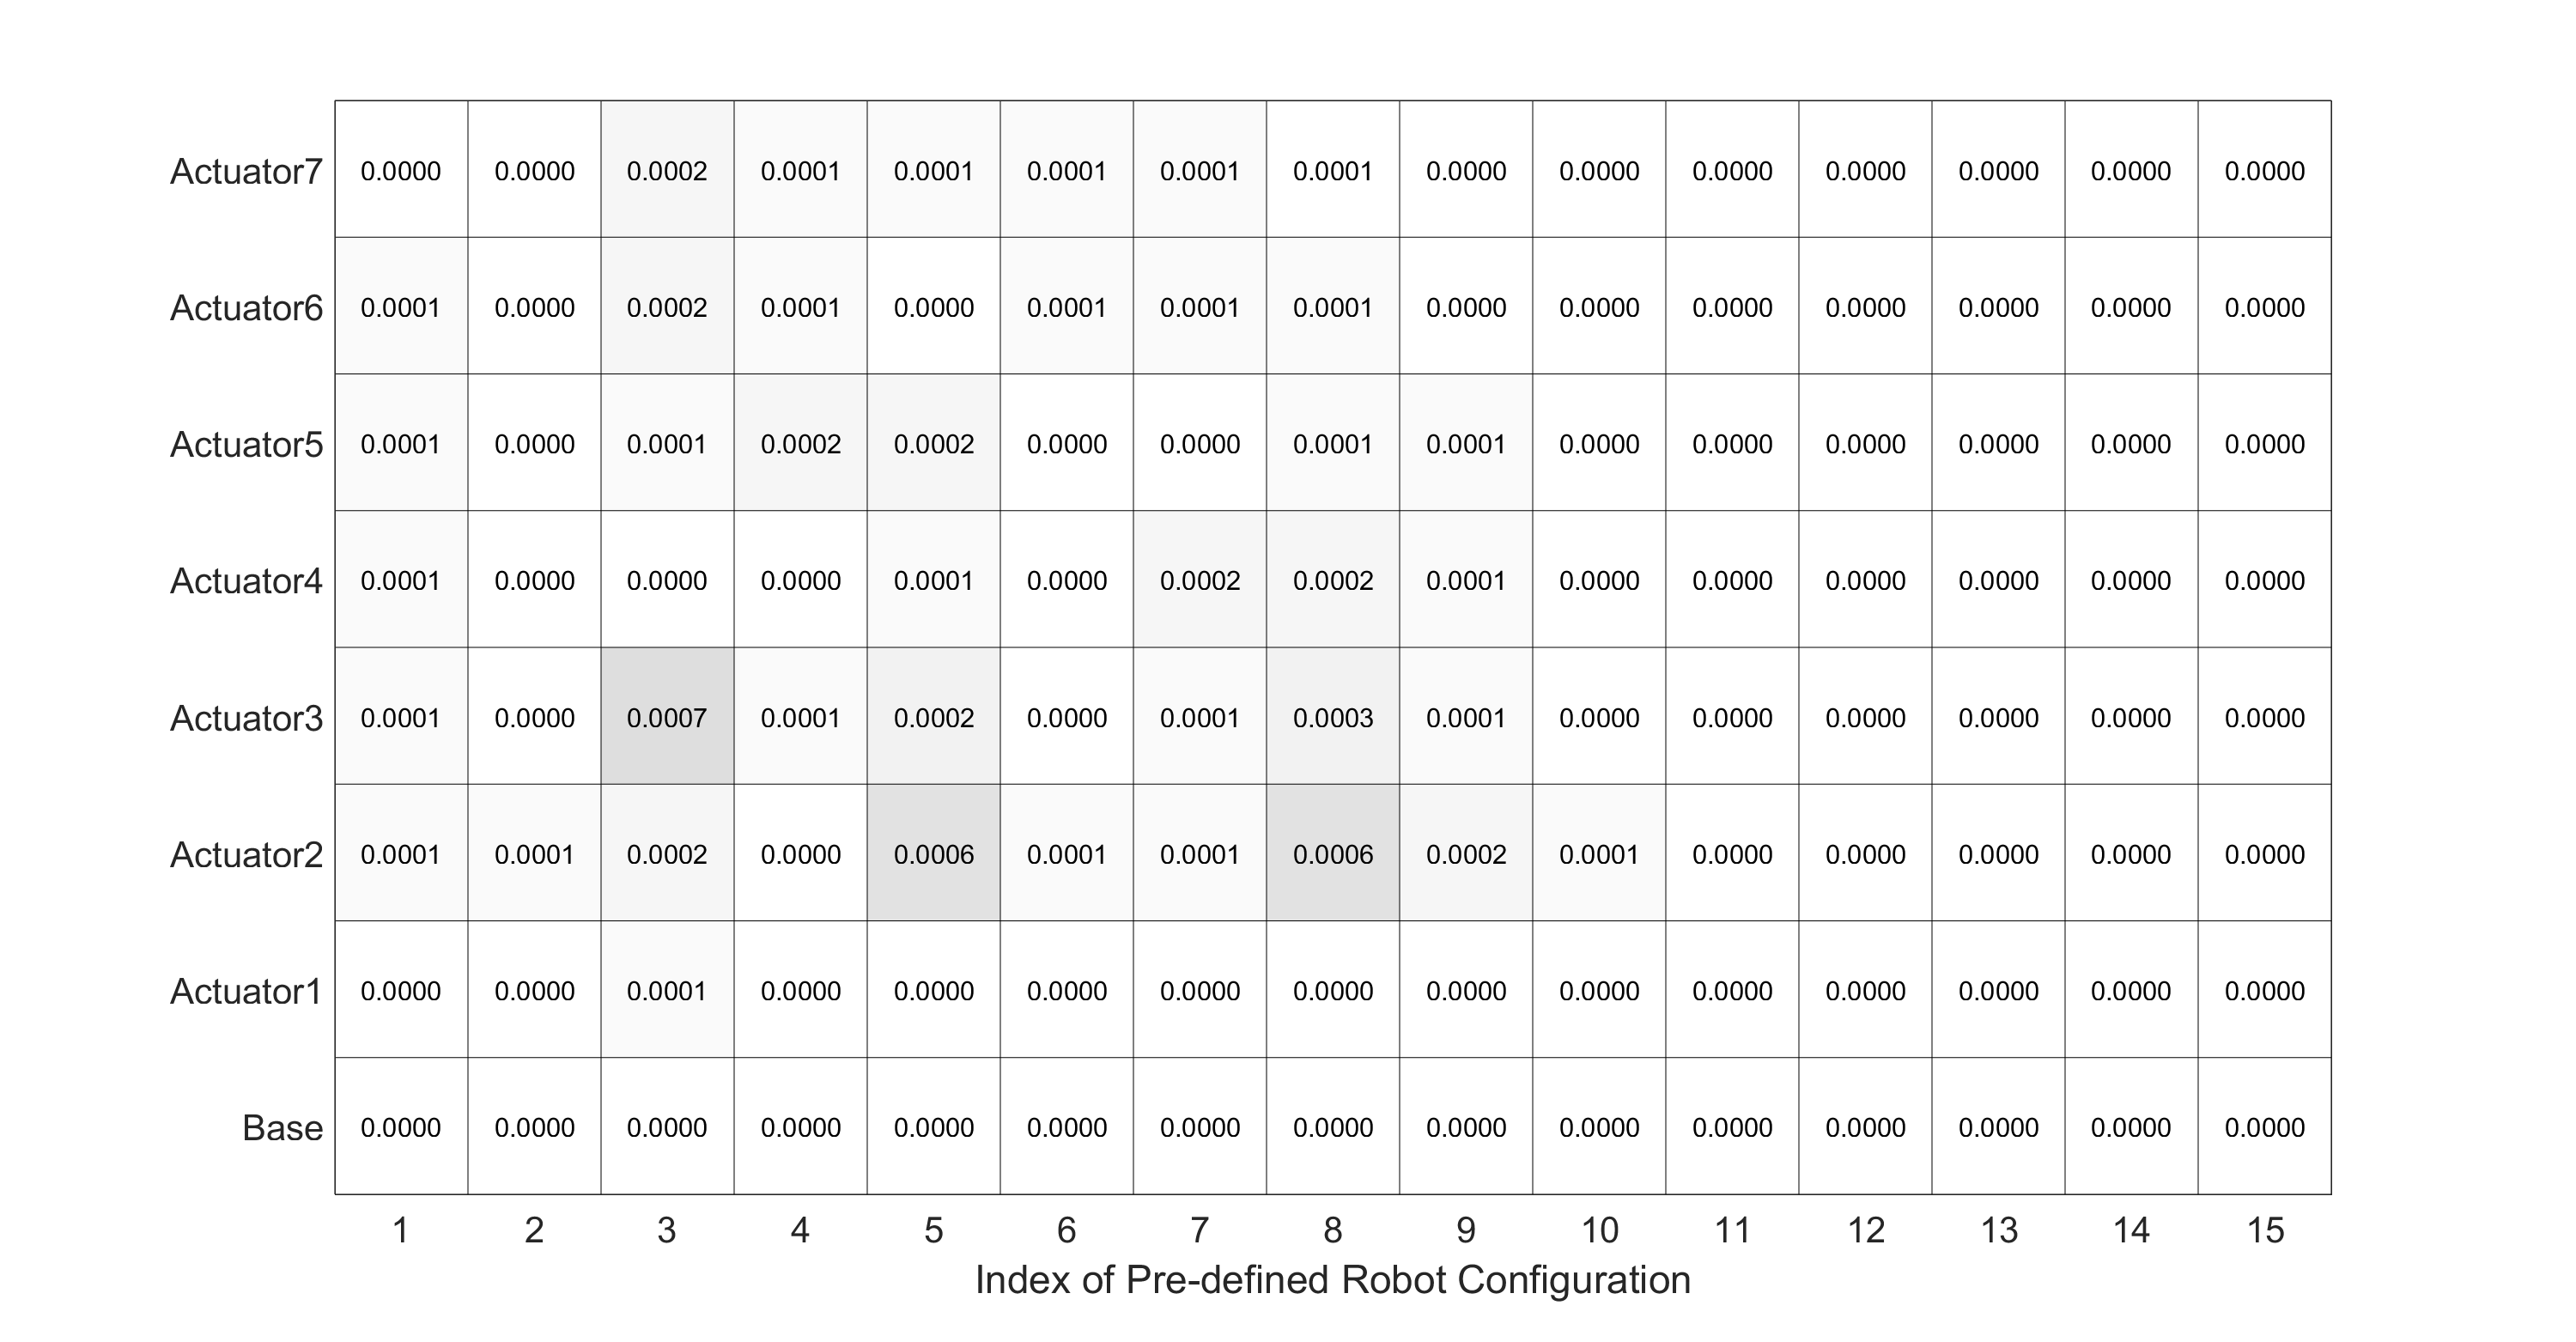
\includegraphics[width=0.9\textwidth]{./images/ForceXErrorFB.png}%
		\caption{Error of Force along X axis in N}
		\label{fig:ForceXErrorFB}%
	\end{center}
\end{figure}

\begin{figure}[H]
	\begin{center}
		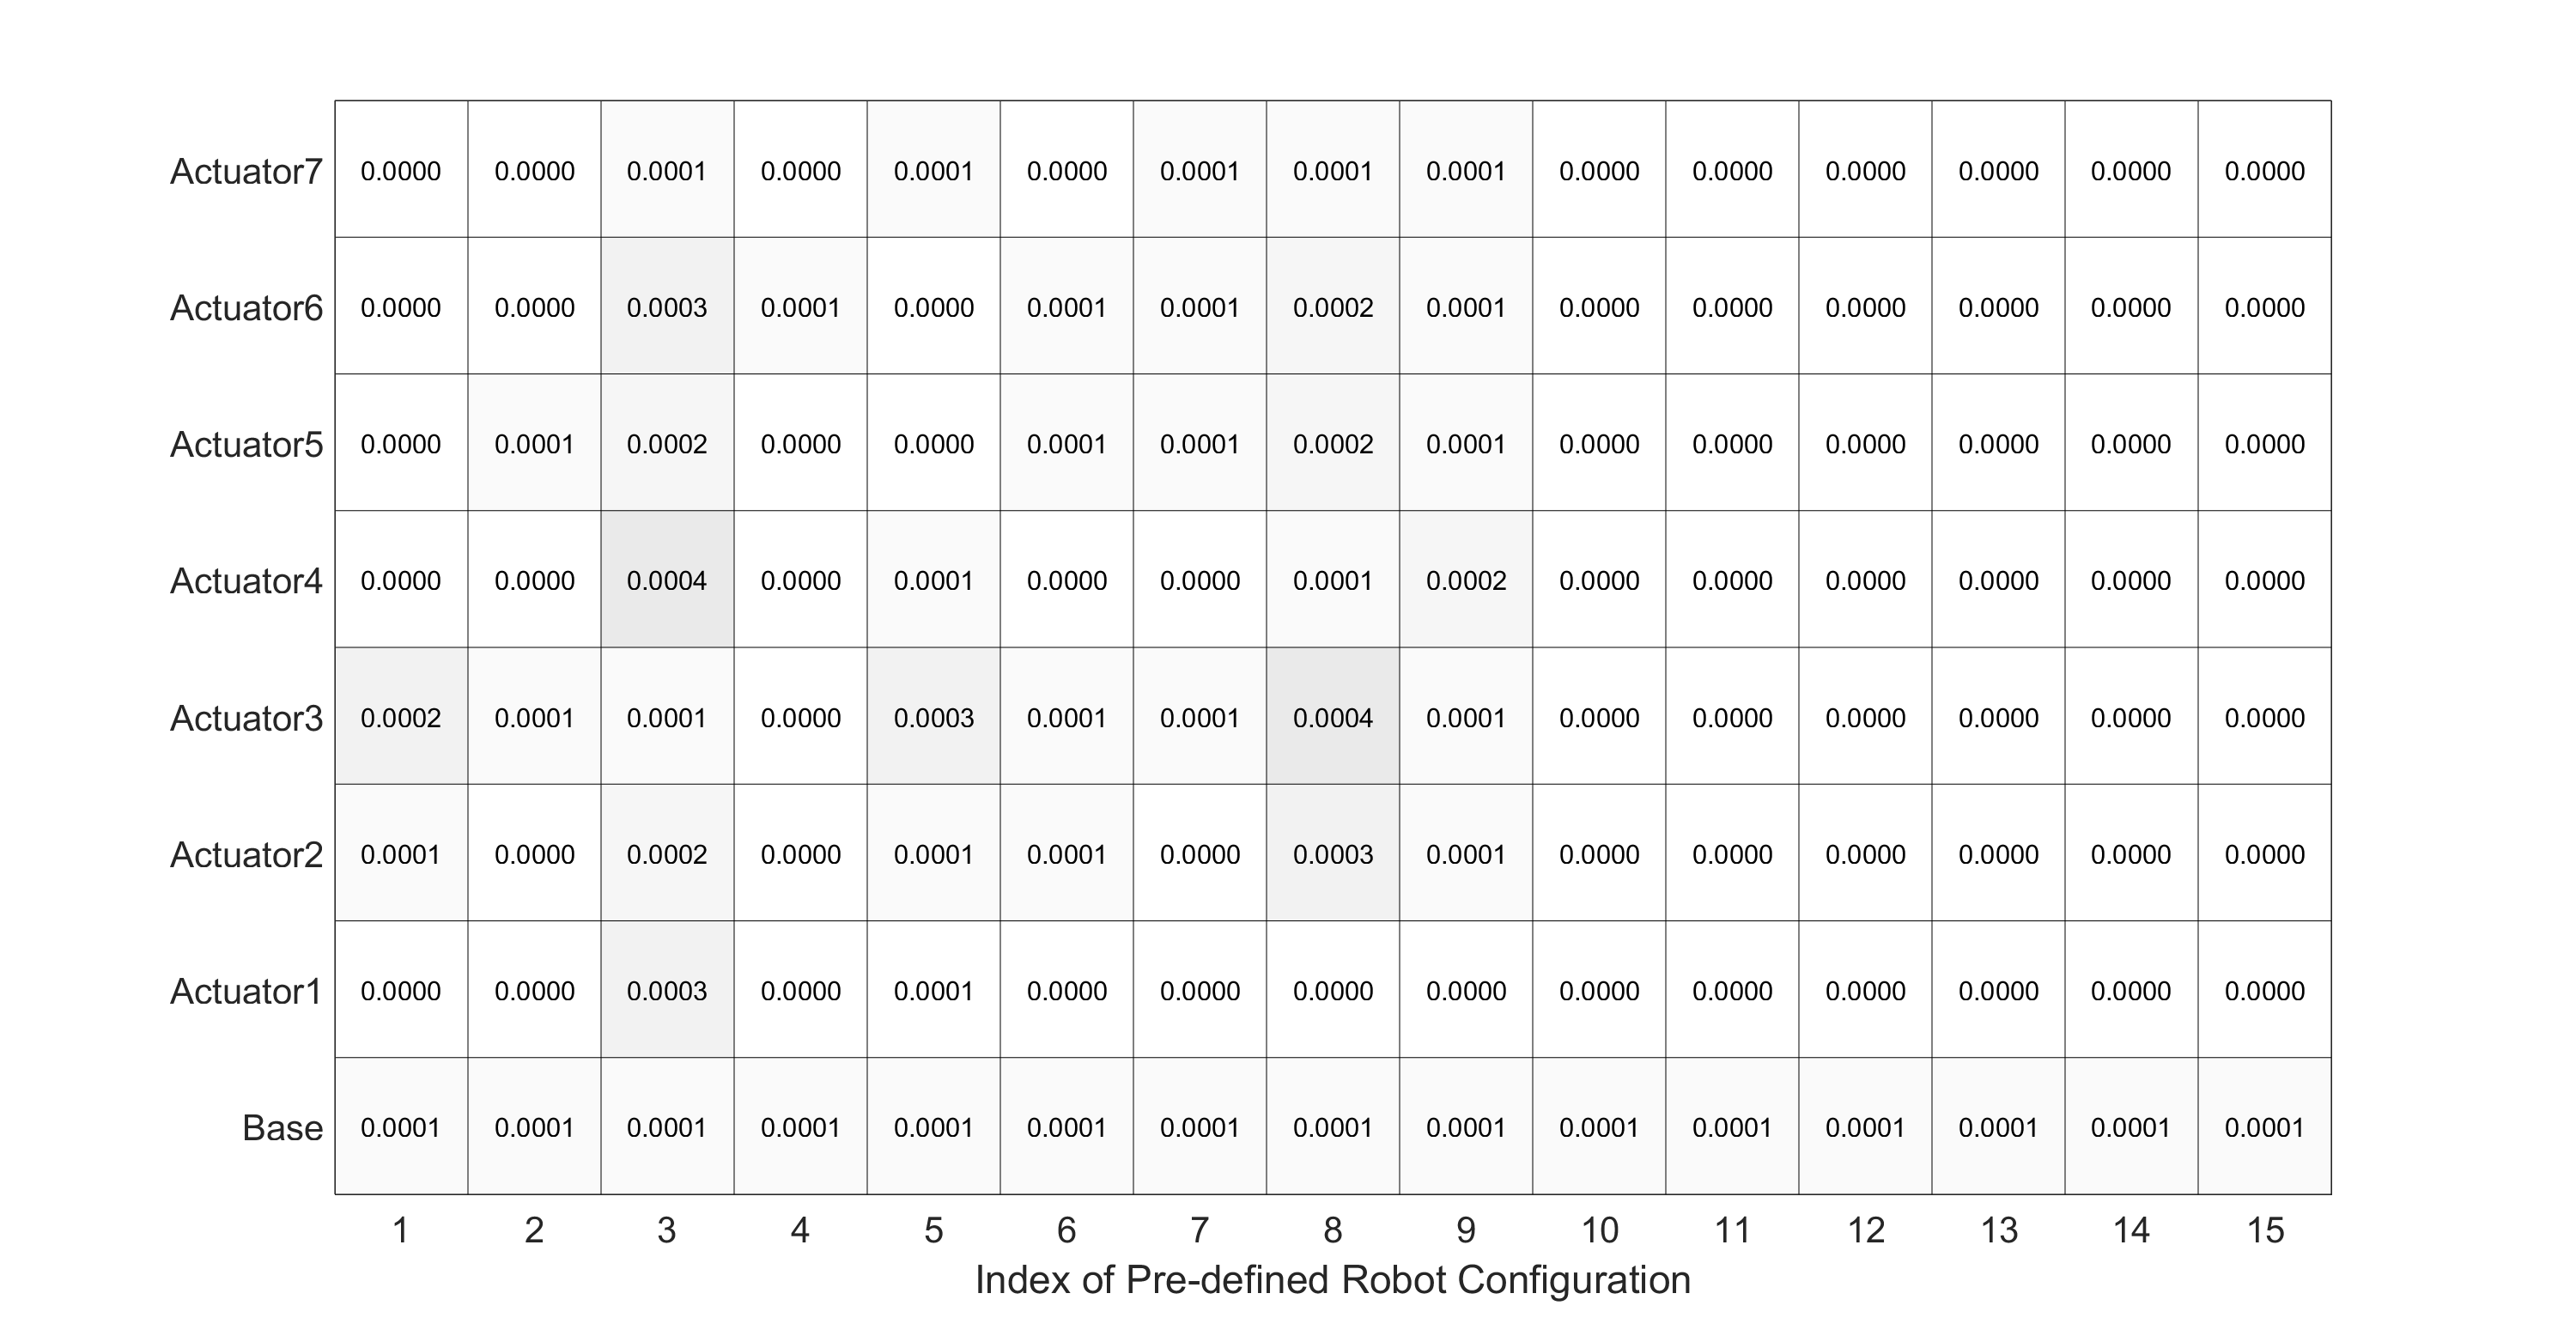
\includegraphics[width=0.9\textwidth]{./images/ForceYErrorFB.png}%
		\caption{Error of Force along Y axis in N}
		\label{fig:ForceYErrorFB}%
	\end{center}
\end{figure}

\begin{figure}[H]
	\begin{center}
		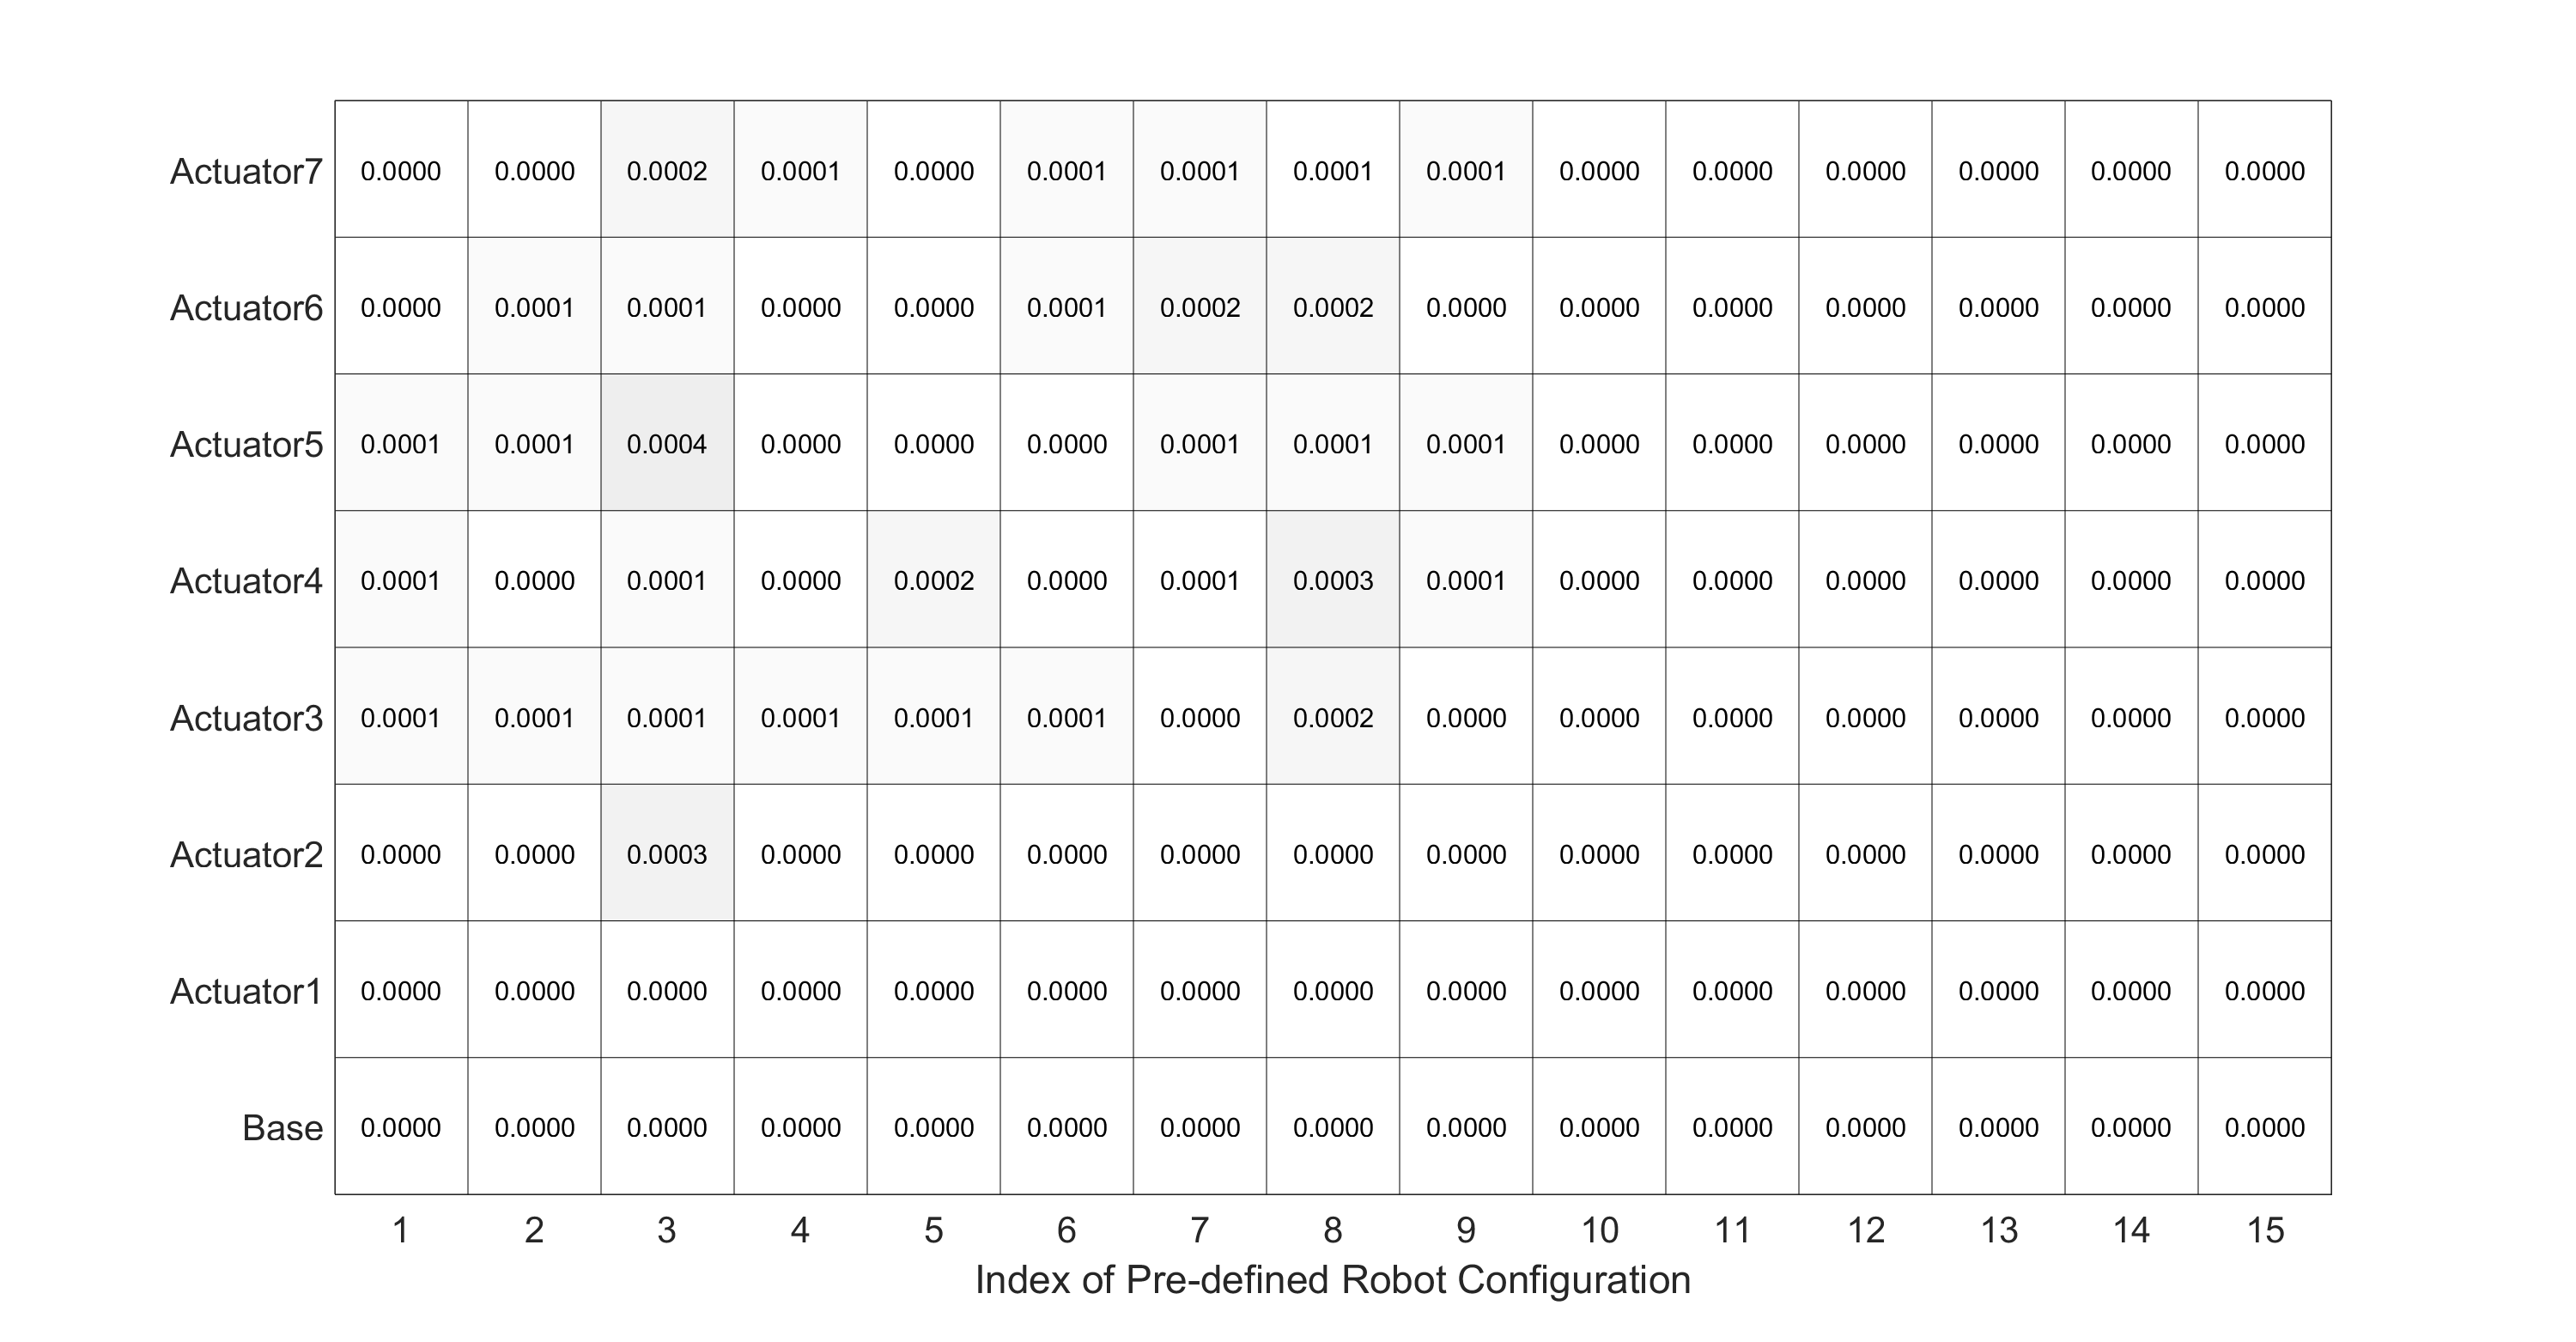
\includegraphics[width=0.9\textwidth]{./images/ForceZErrorFB.png}%
		\caption{Error of Force along Z axis in N}
		\label{fig:ForceZErrorFB}%
	\end{center}
\end{figure}

\begin{figure}[H]
	\begin{center}
		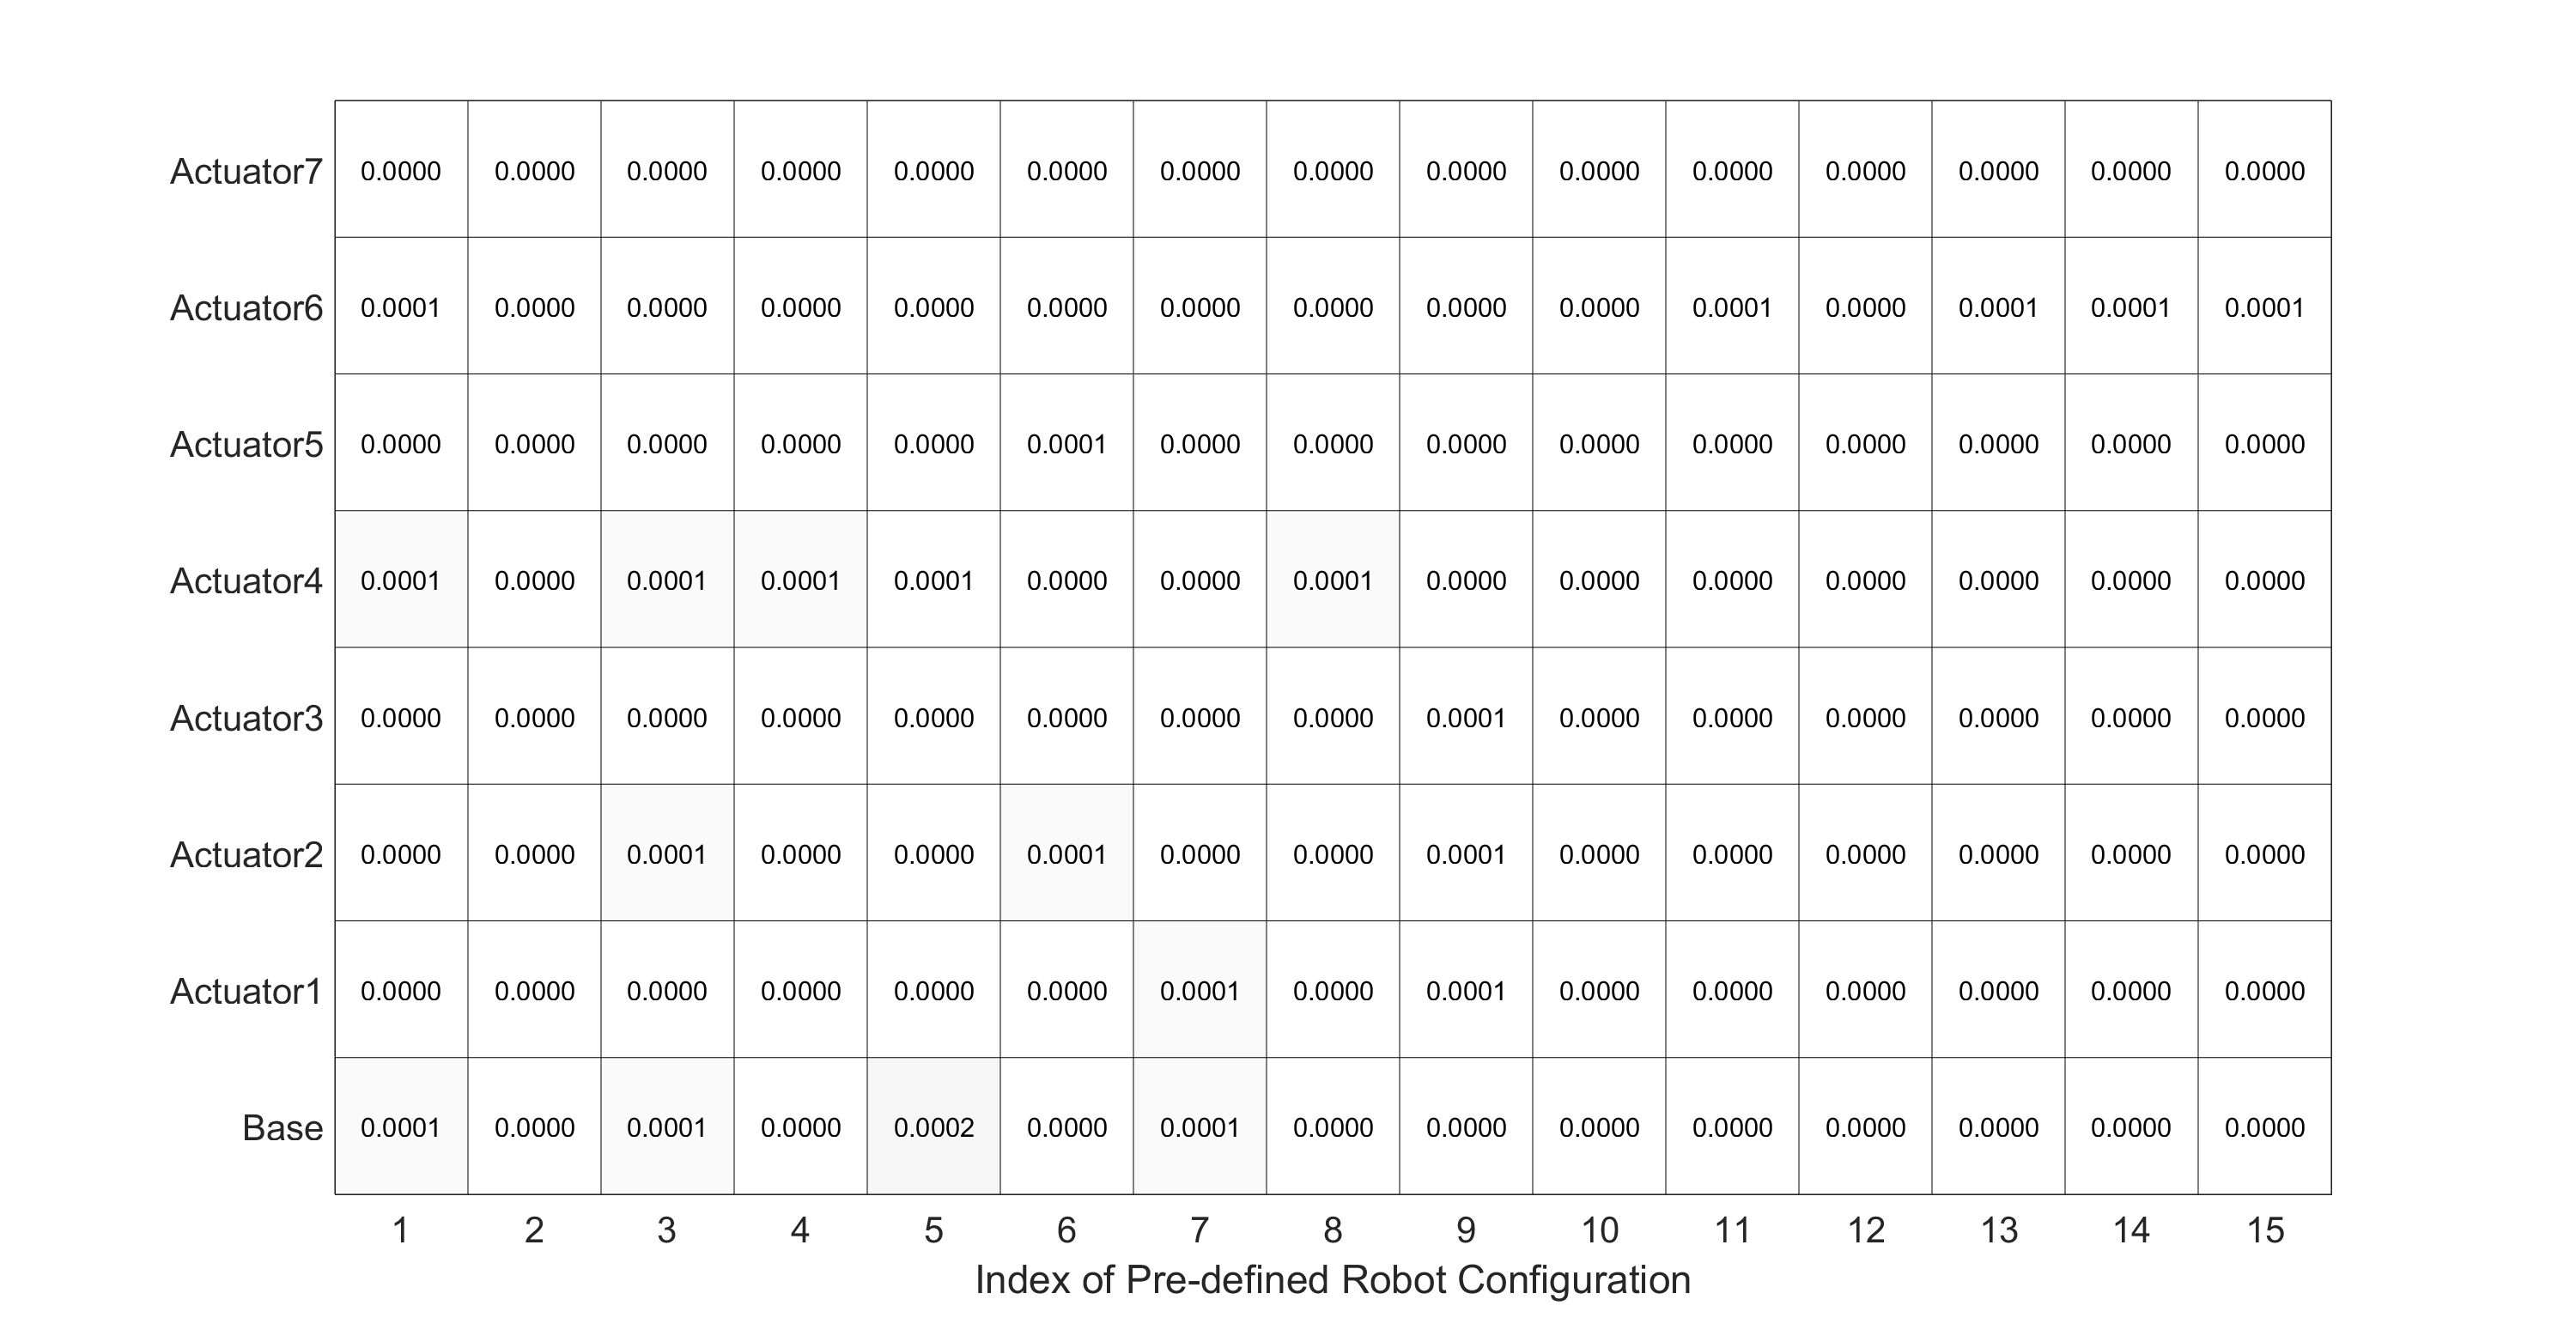
\includegraphics[width=0.9\textwidth]{./images/TorqueXErrorFB.png}%
		\caption{Error of Torque along X axis in Nm}
		\label{fig:TorqueXErrorFB}%
	\end{center}
\end{figure}

\begin{figure}[H]
	\begin{center}
		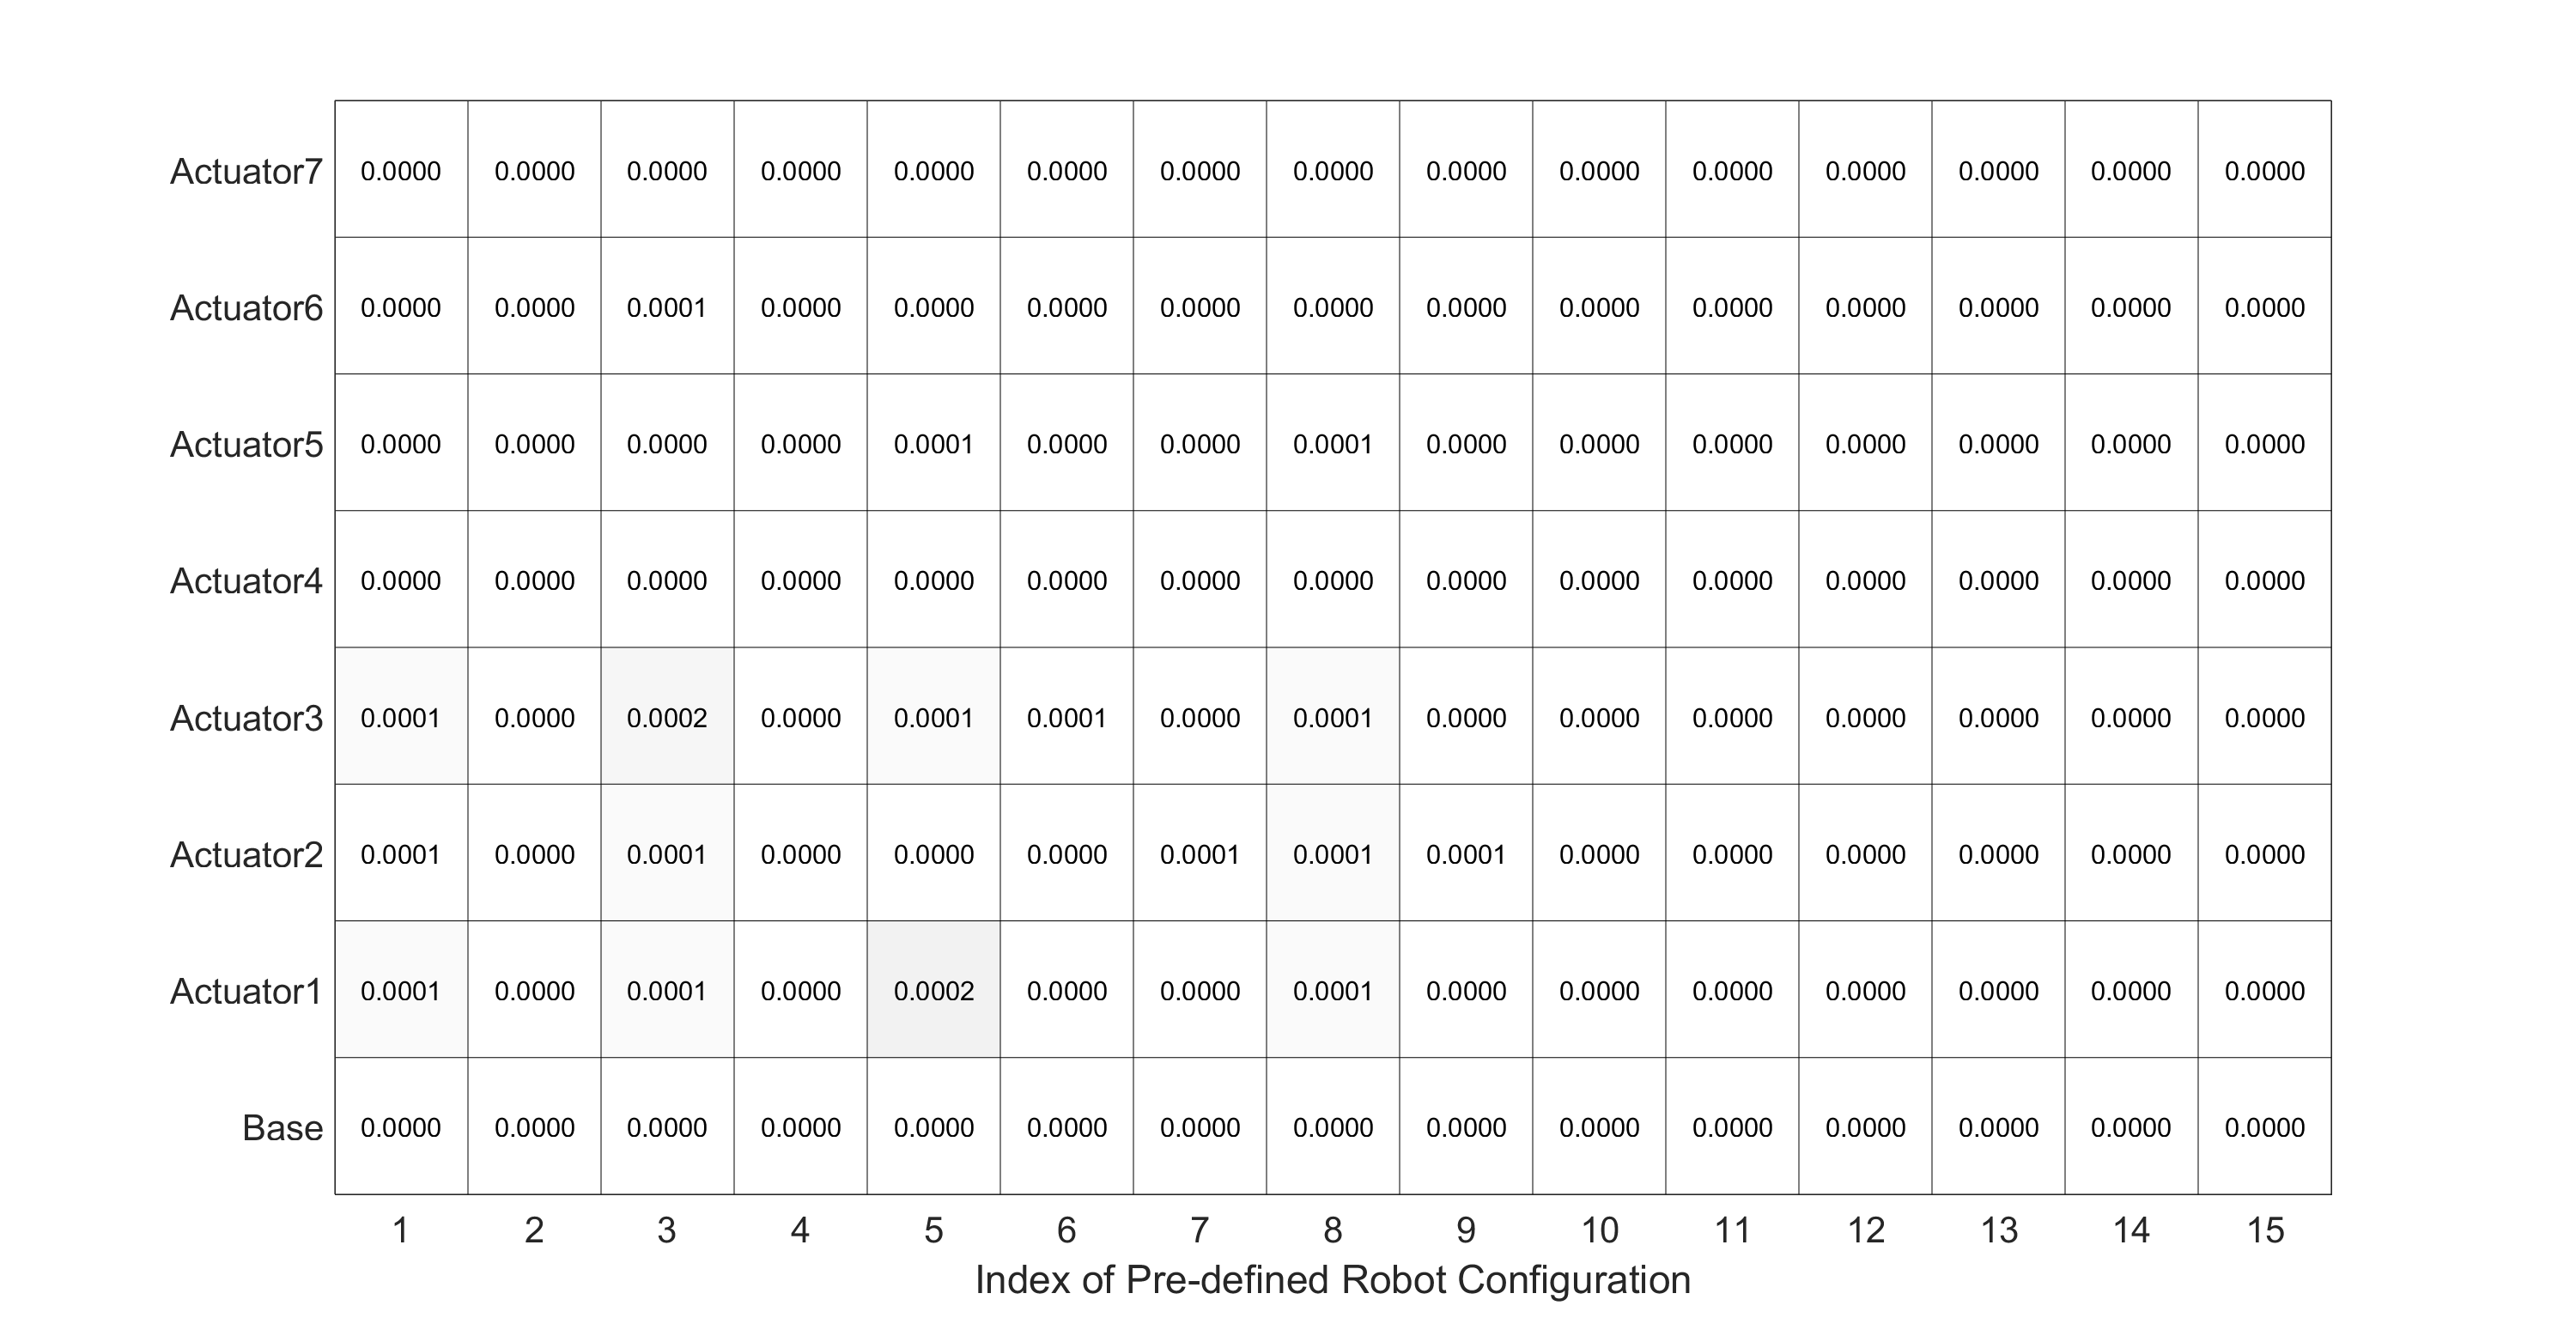
\includegraphics[width=0.9\textwidth]{./images/TorqueYErrorFB.png}%
		\caption{Error of Torque along Y axis in Nm}
		\label{fig:TorqueYErrorFB}%
	\end{center}
\end{figure}

\begin{figure}[H]
	\begin{center}
		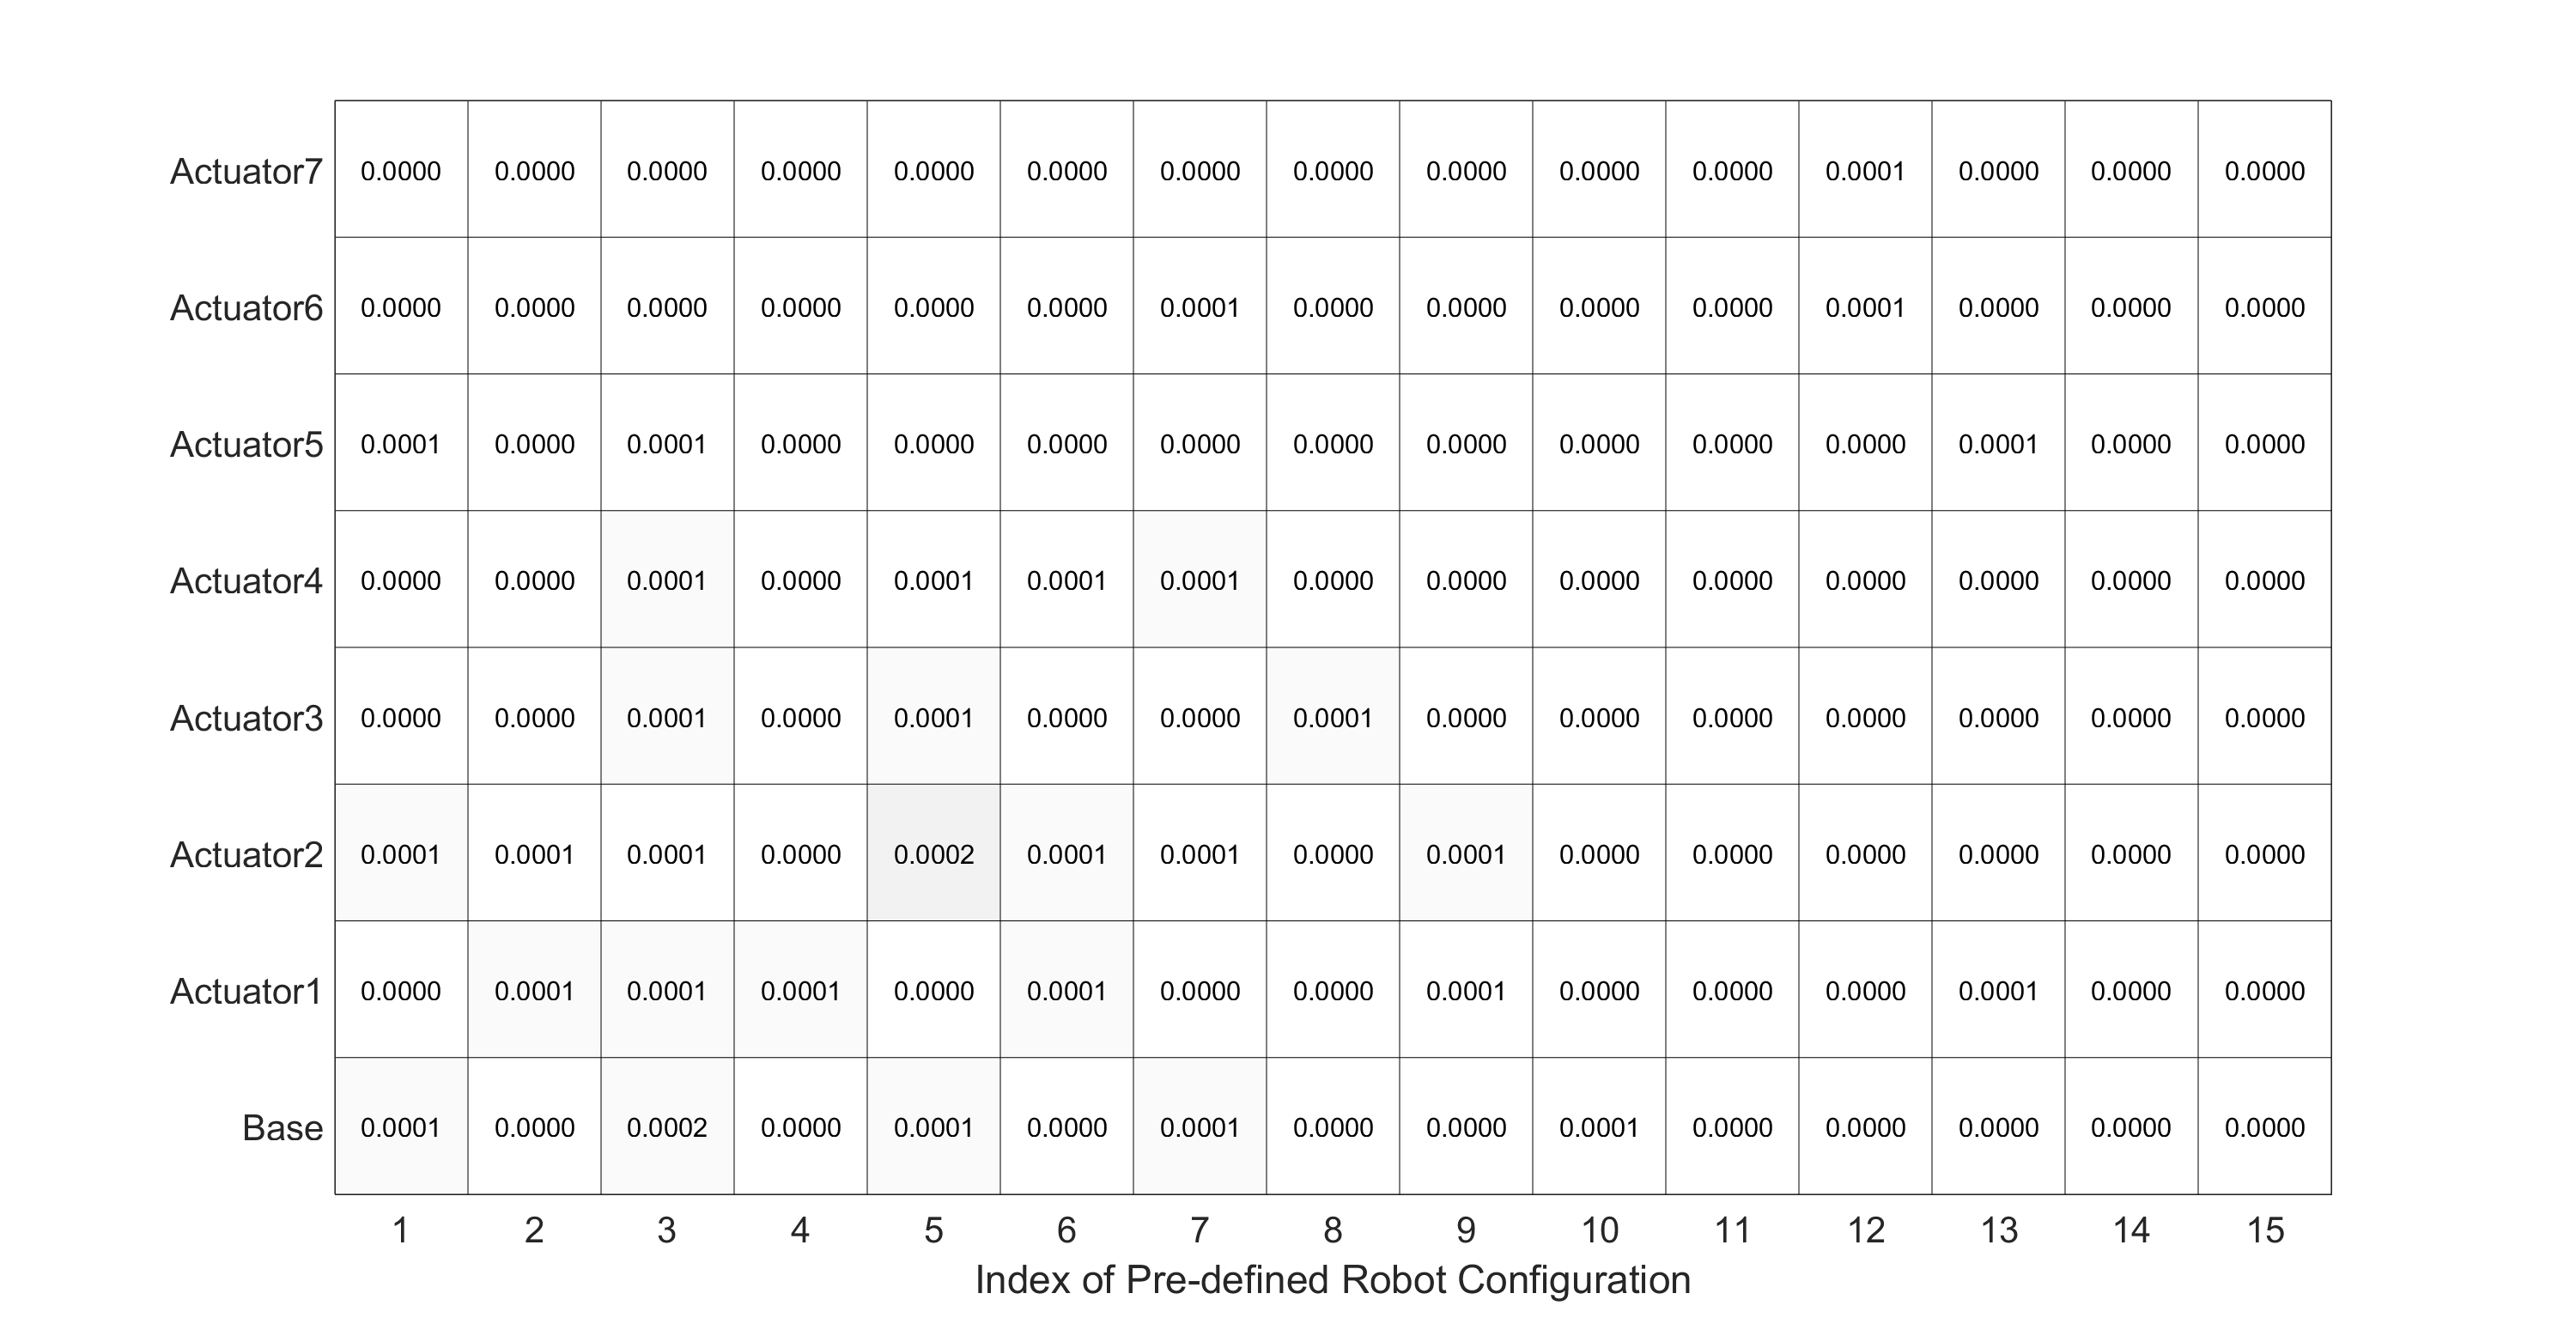
\includegraphics[width=0.9\textwidth]{./images/TorqueZErrorFB.png}%
		\caption{Error of Torque along Z axis in Nm}
		\label{fig:TorqueZErrorFB}%
	\end{center}
\end{figure}

\textbf{Therefore, we can conclude that the joint wrench data from robot base matches with the data from offline PC. The computed joint wrench in robot base performs as designed.}


The joint torque sensors are used to validate the performance of gravity model. Since joint torque sensors only measure the torque along joint axis, only the components of TorqueZ of JointWrench\_Base are used for the comparison. The differences are demonstrated in Figure \ref{fig:SensorErrortoBaseJointWrench}

\begin{figure}[H]
	\begin{center}
		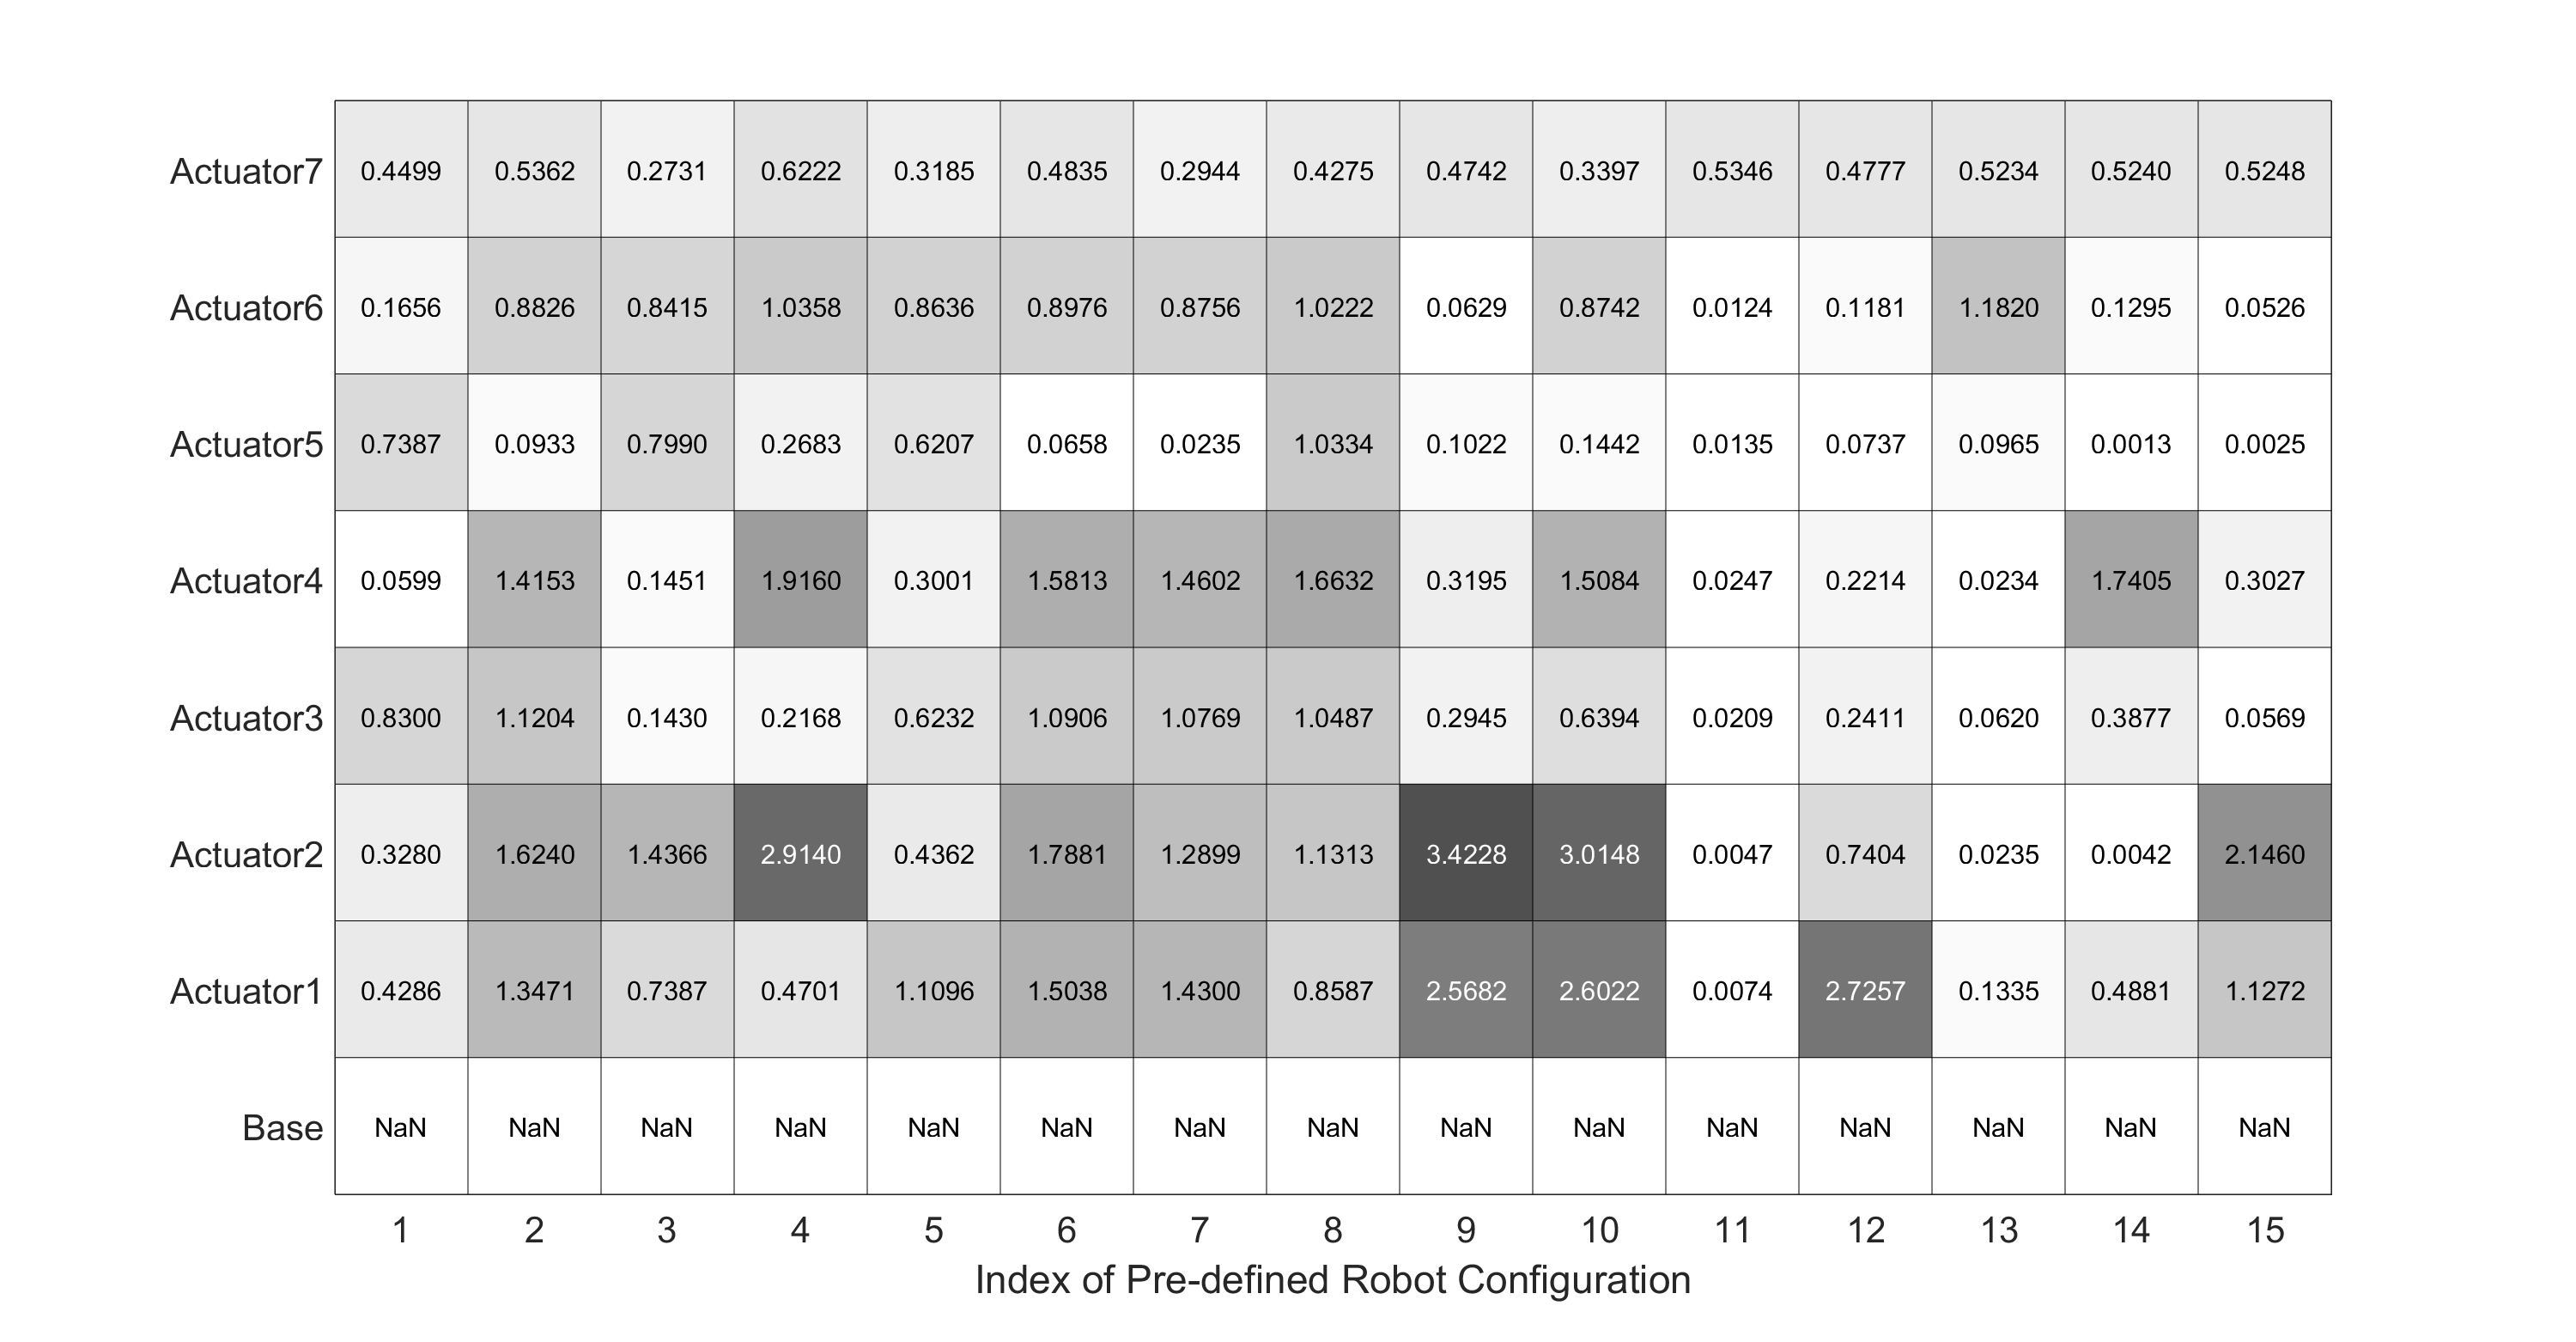
\includegraphics[width=0.9\textwidth]{./images/SensorErrortoBaseJointWrench.png}%
		\caption{Error of Torque along Z axis in Nm}
		\label{fig:SensorErrortoBaseJointWrench}%
	\end{center}
\end{figure}

The row for Base in Figure \ref{fig:SensorErrortoBaseJointWrench} is all NaN since there is no torque sensor on the robot base. The difference between joint torque sensor and  TorqueZ of JointWrench\_Base are quite evident, approximately 3.5Nm in worst cases. However, this is not enough to conclude that gravity model does not function well. The torque sensor is noisy and the seal at each joint may provide additional torque besides gravity torque. We already estimated that the seal may contribute around 2Nm to the joint. The estimation of torque sensor noise will be discussed in the Section \ref{sec:sensorReliability}.




%\section*{Revisions}
%
%\begin{tabular}{|m{0.2\textwidth}|m{0.7\textwidth}|}
%  \hline
%  Date & Changes                                                              \\ \hline
%  2016/01/28 & Initial Version                                                \\ \hline
%\end{tabular}
%

\newpage

\section{Limitations}
% limitation.tex

There are certain limitations for this test.

\begin{enumerate}
	\item NOVA or robot did not provide same/similar data value with the same robot configuration. (eg: Comparing the joint wrench data at the base between Figure \ref{fig:pose6discarded} and Figure \ref{fig:pose6used})
	\item Pose3 is not achievable due to the limit of joint 6. The closest configuration to Pose3 is [293.0001,   137.0502,  220.5201,  87.3998 ,  217.9778,  307.4591,  103.1300], and this data used for the offline computation on PC as well.
	\item Accuracy of Joint Sensor Data (joint sensor data to be added  after torque sensor calibration ...)
\end{enumerate}


\begin{figure}
	\begin{center}
		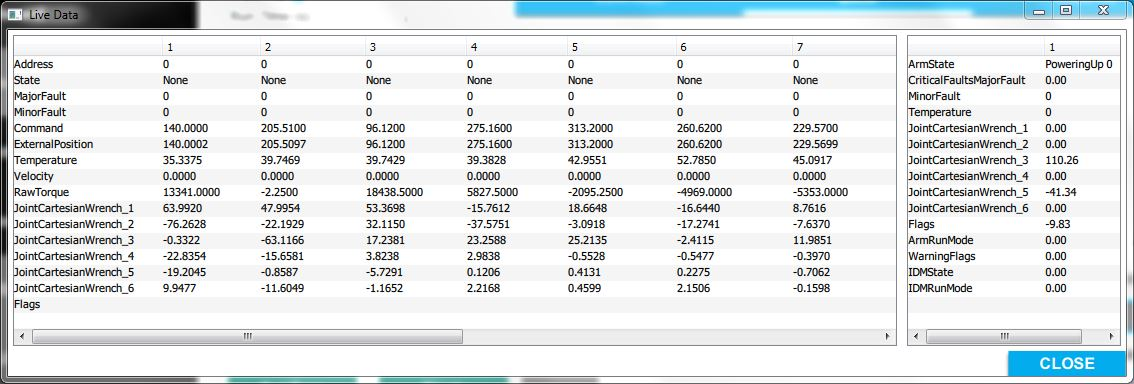
\includegraphics[width=0.9\textwidth]{./images/Pose6}%
		\captionof{figure}{Used Pose6}
		\label{fig:pose6used}
	\end{center}
\end{figure}

\begin{figure}
	\begin{center}
		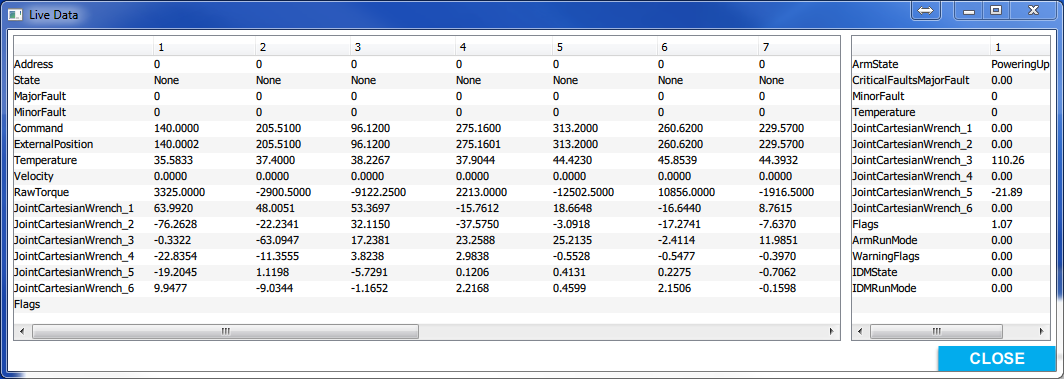
\includegraphics[width=0.9\textwidth]{./images/Pose6_old}%
		\captionof{figure}{Discarded Pose6}
		\label{fig:pose6discarded}
	\end{center}
\end{figure}



\newpage

\section{Appendix}

% start of template --------------------------------------------------------------------------------------------------------------------------------------------------------

\subsection{Test at robot configuration 1}
Robot joint angles are  [ 115        236.85         138.2        264.09            63        235.28        155.28];

\begin{table}[h!]
	\centering
	\caption{Joint wrench obtained from PC (N/Nm)}
	\label{wrech_PC_Pose1}
	\begin{tabular}{|l|r|r|r|r|r|r|r|r|}
		\hline
		\textbf{}  & \textbf{Base} & \textbf{Joint1}  & \textbf{Joint2}  & \textbf{Joint3}  & \textbf{Joint4}  & \textbf{Joint5}  & \textbf{Joint6}  & \textbf{Joint7} \\ \hline
		\textbf{Fx PC}  & 0        & 90.228        & 41.3099        & 42.5445        & -31.7672        & 9.1143        & -10.5665        & 2.2934 \\ \hline
		\textbf{Fy PC}  & 110.2625        & -42.0707        & -62.1115        & 1.1795        & -34.5177        & -19.3155        & -15.8279        & 12.3686 \\ \hline
		\textbf{Fz PC}  & 0        & -0.2484        & -34.8631        & 48.6356        & 0.8023        & 23.1839        & -14.8006        & 10.9768 \\ \hline
		\textbf{Tx PC}  & -27.9005        & -6.9044        & -7.129        & -0.7967        & 0.9116        & -3.1432        & -2.3085        & 1.1963 \\ \hline
		\textbf{Ty PC}  & 0        & -14.8713        & -2.405        & 2.0313        & -0.645        & 0.7029        & 0.0888        & -0.1851 \\ \hline
		\textbf{Tz PC}  & -10.7114        & 10.7851        & -4.1627        & 0.6476        & 8.3476        & 1.8213        & 1.5531        & -0.0414 \\ \hline
	\end{tabular}
\end{table}

\begin{table}[h!]
	\centering
	\caption{Joint wrench obtained from Robot (N/Nm)}
	\label{wrech_Robot_Pose1}
	\begin{tabular}{|l|r|r|r|r|r|r|r|r|}
		\hline
		\textbf{} & \textbf{Base} & \textbf{Joint1}  & \textbf{Joint2}  & \textbf{Joint3}  & \textbf{Joint4}  & \textbf{Joint5}  & \textbf{Joint6}  & \textbf{Joint7} \\ \hline
		\textbf{Fx Robot}  & 0        & 90.2279        & 41.31        & 42.5447        & -31.7672        & 9.1144        & -10.5665        & 2.2934 \\ \hline
		\textbf{Fy Robot}  & 110.26        & -42.071        & -62.1113        & 1.1794        & -34.5177        & -19.3155        & -15.828        & 12.3686 \\ \hline
		\textbf{Fz Robot}  & 0        & -0.2484        & -34.8634        & 48.6355        & 0.8022        & 23.1839        & -14.8006        & 10.9768 \\ \hline
		\textbf{Tx Robot}  & -27.9        & -6.9044        & -7.1291        & -0.7967        & 0.9116        & -3.1432        & -2.3084        & 1.1963 \\ \hline
		\textbf{Ty Robot}  & 0        & -14.8713        & -2.405        & 2.0313        & -0.645        & 0.7028        & 0.0888        & -0.1851 \\ \hline
		\textbf{Tz Robot}  & -10.71        & 10.7852        & -4.1627        & 0.6476        & 8.3476        & 1.8213        & 1.5531        & -0.0414 \\ \hline
	\end{tabular}
\end{table}

\begin{table}[h!]
	\centering
	\caption{Joint wrench error between data from PC and Robot (N/Nm)}
	\label{wrech_Error_Pose1}
	\begin{tabular}{|l|r|r|r|r|r|r|r|r|}
		\hline
		\textbf{}  & \textbf{Base} & \textbf{Joint1}  & \textbf{Joint2}  & \textbf{Joint3}  & \textbf{Joint4}  & \textbf{Joint5}  & \textbf{Joint6}  & \textbf{Joint7} \\ \hline
		\textbf{Fx Error}  & 0        & 0.0001        & -0.0001        & -0.0002        & 0        & -0.0001        & 0        & 0 \\ \hline
		\textbf{Fy Error}  & 0.0025        & 0.0003        & -0.0002        & 0.0001        & 0        & 0        & 0.0001        & 0 \\ \hline
		\textbf{Fz Error}  & 0        & 0        & 0.0003        & 0.0001        & 0.0001        & 0        & 0        & 0 \\ \hline
		\textbf{Tx Error}  & -0.0005        & 0        & 0.0001        & 0        & 0        & 0        & -0.0001        & 0 \\ \hline
		\textbf{Ty Error}  & 0        & 0        & 0        & 0        & 0        & 0.0001        & 0        & 0 \\ \hline
		\textbf{Tz Error}  & -0.0014        & -0.0001        & 0        & 0        & 0        & 0        & 0        & 0 \\ \hline
	\end{tabular}
\end{table}

\begin{table}[h!]
	\centering
	\caption{Joint torque along axis comparison with sensor data (Nm)}
	\label{wrech_Sensor_Pose1}
	\begin{tabular}{|l|r|r|r|r|r|r|r|}
		\hline
		\textbf{} & \textbf{Joint1} & \textbf{Joint2} & \textbf{Joint3} & \textbf{Joint4} & \textbf{Joint5} & \textbf{Joint6} & \textbf{Joint7} \\ \hline
		\textbf{Tz Sensor}  & 0           & 0           & 0            & 0           & 0           & 0           & 0           \\ \hline
		\textbf{Tz Robot}  	& 10.7852           & -4.1627           & 0.6476            & 8.3476           & 1.8213           & 1.5531           & -0.0414           \\ \hline
		\textbf{Tz PC}  	& 10.7851           & -4.1627           & 0.6476            & 8.3476           & 1.8213           & 1.5531           & -0.0414           \\ \hline
	\end{tabular}
\end{table}

% end of template --------------------------------------------------------------------------------------------------------------------------------------------------------
% start of template --------------------------------------------------------------------------------------------------------------------------------------------------------

\subsection{Test at robot configuration 2}
Robot joint angles are  [ 140        245.42         90.92        281.41        353.62        295.06         265.4];

\begin{table}[h!]
	\centering
	\caption{Joint wrench obtained from PC (N/Nm)}
	\label{wrech_PC_Pose2}
	\begin{tabular}{|l|r|r|r|r|r|r|r|r|}
		\hline
		\textbf{}  & \textbf{Base} & \textbf{Joint1}  & \textbf{Joint2}  & \textbf{Joint3}  & \textbf{Joint4}  & \textbf{Joint5}  & \textbf{Joint6}  & \textbf{Joint7} \\ \hline
		\textbf{Fx PC}  & 0        & 64.0037        & 22.469        & 49.9289        & -33.653        & 23.3638        & -21.6473        & 4.3091 \\ \hline
		\textbf{Fy PC}  & 110.2625        & -76.2533        & -47.8244        & 16.84        & -30.3433        & -5.7106        & -9.648        & -14.6683 \\ \hline
		\textbf{Fz PC}  & 0        & -0.2559        & -63.1487        & 37.4215        & 12.1667        & 20.3759        & -4.4205        & 6.7086 \\ \hline
		\textbf{Tx PC}  & -29.0945        & -13.4362        & -13.4574        & 0.3224        & 1.4061        & -0.3649        & -0.6654        & -1.0595 \\ \hline
		\textbf{Ty PC}  & 0        & -11.3291        & -1.3893        & -1.9633        & 0.6292        & 0.7207        & 0.167        & -0.3473 \\ \hline
		\textbf{Tz PC}  & -15.2101        & 15.2878        & -3.7361        & 0.4533        & 5.4584        & 0.6204        & 2.894        & -0.0789 \\ \hline
	\end{tabular}
\end{table}

\begin{table}[h!]
	\centering
	\caption{Joint wrench obtained from Robot (N/Nm)}
	\label{wrech_Robot_Pose2}
	\begin{tabular}{|l|r|r|r|r|r|r|r|r|}
		\hline
		\textbf{} & \textbf{Base} & \textbf{Joint1}  & \textbf{Joint2}  & \textbf{Joint3}  & \textbf{Joint4}  & \textbf{Joint5}  & \textbf{Joint6}  & \textbf{Joint7} \\ \hline
		\textbf{Fx Robot}  & 0        & 64.0034        & 22.4689        & 49.9291        & -33.6529        & 23.3637        & -21.6474        & 4.3091 \\ \hline
		\textbf{Fy Robot}  & 110.26        & -76.2536        & -47.8241        & 16.84        & -30.3434        & -5.7106        & -9.648        & -14.6683 \\ \hline
		\textbf{Fz Robot}  & 0        & -0.2559        & -63.1489        & 37.4213        & 12.1667        & 20.376        & -4.4204        & 6.7086 \\ \hline
		\textbf{Tx Robot}  & -29.09        & -13.4363        & -13.4575        & 0.3224        & 1.4061        & -0.3649        & -0.6654        & -1.0595 \\ \hline
		\textbf{Ty Robot}  & 0        & -11.329        & -1.3893        & -1.9634        & 0.6292        & 0.7207        & 0.167        & -0.3473 \\ \hline
		\textbf{Tz Robot}  & -15.21        & 15.2879        & -3.7361        & 0.4534        & 5.4584        & 0.6204        & 2.894        & -0.0789 \\ \hline
	\end{tabular}
\end{table}

\begin{table}[h!]
	\centering
	\caption{Joint wrench error between data from PC and Robot (N/Nm)}
	\label{wrech_Error_Pose2}
	\begin{tabular}{|l|r|r|r|r|r|r|r|r|}
		\hline
		\textbf{}  & \textbf{Base} & \textbf{Joint1}  & \textbf{Joint2}  & \textbf{Joint3}  & \textbf{Joint4}  & \textbf{Joint5}  & \textbf{Joint6}  & \textbf{Joint7} \\ \hline
		\textbf{Fx Error}  & 0        & 0.0003        & 0.0001        & -0.0002        & -0.0001        & 0.0001        & 0.0001        & 0 \\ \hline
		\textbf{Fy Error}  & 0.0025        & 0.0003        & -0.0003        & 0        & 0.0001        & 0        & 0        & 0 \\ \hline
		\textbf{Fz Error}  & 0        & 0        & 0.0002        & 0.0002        & 0        & -0.0001        & -0.0001        & 0 \\ \hline
		\textbf{Tx Error}  & -0.0045        & 0.0001        & 0.0001        & 0        & 0        & 0        & 0        & 0 \\ \hline
		\textbf{Ty Error}  & 0        & -0.0001        & 0        & 0.0001        & 0        & 0        & 0        & 0 \\ \hline
		\textbf{Tz Error}  & -0.0001        & -0.0001        & 0        & -0.0001        & 0        & 0        & 0        & 0 \\ \hline
	\end{tabular}
\end{table}

\begin{table}[h!]
	\centering
	\caption{Joint torque along axis comparison with sensor data (Nm)}
	\label{wrech_Sensor_Pose2}
	\begin{tabular}{|l|r|r|r|r|r|r|r|}
		\hline
		\textbf{} & \textbf{Joint1} & \textbf{Joint2} & \textbf{Joint3} & \textbf{Joint4} & \textbf{Joint5} & \textbf{Joint6} & \textbf{Joint7} \\ \hline
		\textbf{Tz Sensor}  & 0           & 0           & 0            & 0           & 0           & 0           & 0           \\ \hline
		\textbf{Tz Robot}  	& 15.2879           & -3.7361           & 0.4534            & 5.4584           & 0.6204           & 2.894           & -0.0789           \\ \hline
		\textbf{Tz PC}  	& 15.2878           & -3.7361           & 0.4533            & 5.4584           & 0.6204           & 2.894           & -0.0789           \\ \hline
	\end{tabular}
\end{table}

% end of template --------------------------------------------------------------------------------------------------------------------------------------------------------
% start of template --------------------------------------------------------------------------------------------------------------------------------------------------------

\subsection{Test at robot configuration 3}
Robot joint angles are  [ 293.0001      137.0502      220.5201       87.3998      217.9778      307.4591        103.13];

\begin{table}[h!]
	\centering
	\caption{Joint wrench obtained from PC (N/Nm)}
	\label{wrech_PC_Pose3}
	\begin{tabular}{|l|r|r|r|r|r|r|r|r|}
		\hline
		\textbf{}  & \textbf{Base} & \textbf{Joint1}  & \textbf{Joint2}  & \textbf{Joint3}  & \textbf{Joint4}  & \textbf{Joint5}  & \textbf{Joint6}  & \textbf{Joint7} \\ \hline
		\textbf{Fx PC}  & 0        & -91.6344        & -55.4598        & -16.4767        & 30.0831        & 30.2296        & -18.1765        & 5.7336 \\ \hline
		\textbf{Fy PC}  & 110.2625        & 38.9123        & -51.6547        & 47.4566        & -10.4017        & 5.7477        & -15.2318        & 11.5782 \\ \hline
		\textbf{Fz PC}  & 0        & -0.2802        & 32.1837        & 40.6601        & 34.4686        & 6.8404        & 4.3407        & 10.5737 \\ \hline
		\textbf{Tx PC}  & -33.004        & 8.4005        & 8.152        & 4.6381        & 6.1296        & 0.0993        & 0.5016        & 1.1253 \\ \hline
		\textbf{Ty PC}  & 0        & 19.8137        & -3.1897        & -3.1387        & -0.7688        & -0.094        & 0.176        & -0.4622 \\ \hline
		\textbf{Tz PC}  & -4.2674        & 4.3582        & 8.9284        & 5.5428        & -5.5817        & -0.3598        & 2.7181        & -0.1041 \\ \hline
	\end{tabular}
\end{table}

\begin{table}[h!]
	\centering
	\caption{Joint wrench obtained from Robot (N/Nm)}
	\label{wrech_Robot_Pose3}
	\begin{tabular}{|l|r|r|r|r|r|r|r|r|}
		\hline
		\textbf{} & \textbf{Base} & \textbf{Joint1}  & \textbf{Joint2}  & \textbf{Joint3}  & \textbf{Joint4}  & \textbf{Joint5}  & \textbf{Joint6}  & \textbf{Joint7} \\ \hline
		\textbf{Fx Robot}  & 0        & -91.6344        & -55.4597        & -16.4767        & 30.0831        & 30.2296        & -18.1765        & 5.7336 \\ \hline
		\textbf{Fy Robot}  & 110.26        & 38.9123        & -51.6547        & 47.4566        & -10.4016        & 5.7477        & -15.2318        & 11.5781 \\ \hline
		\textbf{Fz Robot}  & 0        & -0.2802        & 32.1838        & 40.6601        & 34.4686        & 6.8403        & 4.3407        & 10.5737 \\ \hline
		\textbf{Tx Robot}  & -33        & 8.4005        & 8.152        & 4.6381        & 6.1296        & 0.0993        & 0.5016        & 1.1253 \\ \hline
		\textbf{Ty Robot}  & 0        & 19.8136        & -3.1897        & -3.1387        & -0.7688        & -0.094        & 0.176        & -0.4622 \\ \hline
		\textbf{Tz Robot}  & -4.27        & 4.3583        & 8.9284        & 5.5428        & -5.5817        & -0.3598        & 2.7181        & -0.1041 \\ \hline
	\end{tabular}
\end{table}

\begin{table}[h!]
	\centering
	\caption{Joint wrench error between data from PC and Robot (N/Nm)}
	\label{wrech_Error_Pose3}
	\begin{tabular}{|l|r|r|r|r|r|r|r|r|}
		\hline
		\textbf{}  & \textbf{Base} & \textbf{Joint1}  & \textbf{Joint2}  & \textbf{Joint3}  & \textbf{Joint4}  & \textbf{Joint5}  & \textbf{Joint6}  & \textbf{Joint7} \\ \hline
		\textbf{Fx Error}  & 0        & 0        & -0.0001        & 0        & 0        & 0        & 0        & 0 \\ \hline
		\textbf{Fy Error}  & 0.0025        & 0        & 0        & 0        & -0.0001        & 0        & 0        & 0.0001 \\ \hline
		\textbf{Fz Error}  & 0        & 0        & -0.0001        & 0        & 0        & 0.0001        & 0        & 0 \\ \hline
		\textbf{Tx Error}  & -0.004        & 0        & 0        & 0        & 0        & 0        & 0        & 0 \\ \hline
		\textbf{Ty Error}  & 0        & 0.0001        & 0        & 0        & 0        & 0        & 0        & 0 \\ \hline
		\textbf{Tz Error}  & 0.0026        & -0.0001        & 0        & 0        & 0        & 0        & 0        & 0 \\ \hline
	\end{tabular}
\end{table}

\begin{table}[h!]
	\centering
	\caption{Joint torque along axis comparison with sensor data (Nm)}
	\label{wrech_Sensor_Pose3}
	\begin{tabular}{|l|r|r|r|r|r|r|r|}
		\hline
		\textbf{} & \textbf{Joint1} & \textbf{Joint2} & \textbf{Joint3} & \textbf{Joint4} & \textbf{Joint5} & \textbf{Joint6} & \textbf{Joint7} \\ \hline
		\textbf{Tz Sensor}  & 0           & 0           & 0            & 0           & 0           & 0           & 0           \\ \hline
		\textbf{Tz Robot}  	& 4.3583           & 8.9284           & 5.5428            & -5.5817           & -0.3598           & 2.7181           & -0.1041           \\ \hline
		\textbf{Tz PC}  	& 4.3582           & 8.9284           & 5.5428            & -5.5817           & -0.3598           & 2.7181           & -0.1041           \\ \hline
	\end{tabular}
\end{table}

% end of template --------------------------------------------------------------------------------------------------------------------------------------------------------
% start of template --------------------------------------------------------------------------------------------------------------------------------------------------------

\subsection{Test at robot configuration 4}
Robot joint angles are  [ 10        176.73        147.59         43.32        142.68           275        205.12];

\begin{table}[h!]
	\centering
	\caption{Joint wrench obtained from PC (N/Nm)}
	\label{wrech_PC_Pose4}
	\begin{tabular}{|l|r|r|r|r|r|r|r|r|}
		\hline
		\textbf{}  & \textbf{Base} & \textbf{Joint1}  & \textbf{Joint2}  & \textbf{Joint3}  & \textbf{Joint4}  & \textbf{Joint5}  & \textbf{Joint6}  & \textbf{Joint7} \\ \hline
		\textbf{Fx PC}  & 0        & 17.2851        & 14.3259        & -24.4358        & 12.4384        & -11.0271        & -5.634        & -2.7765 \\ \hline
		\textbf{Fy PC}  & 110.2625        & 98.042        & 1.1273        & 59.8232        & -12.5632        & 28.3432        & 8.8952        & -15.2768 \\ \hline
		\textbf{Fz PC}  & 0        & -0.3135        & 81.0758        & -0.9653        & 43.4595        & 8.2899        & 21.6879        & -6.1352 \\ \hline
		\textbf{Tx PC}  & -38.347        & 26.441        & 15.372        & 2.9876        & 10.6354        & 2.4216        & 3.16        & -1.3424 \\ \hline
		\textbf{Ty PC}  & 0        & -4.6275        & -9.0529        & 1.3559        & 2.6477        & 1.8578        & -0.0349        & 0.2239 \\ \hline
		\textbf{Tz PC}  & -10.5508        & 10.6594        & -2.5903        & 8.4035        & -2.2785        & -3.1305        & 0.8352        & 0.0501 \\ \hline
	\end{tabular}
\end{table}

\begin{table}[h!]
	\centering
	\caption{Joint wrench obtained from Robot (N/Nm)}
	\label{wrech_Robot_Pose4}
	\begin{tabular}{|l|r|r|r|r|r|r|r|r|}
		\hline
		\textbf{} & \textbf{Base} & \textbf{Joint1}  & \textbf{Joint2}  & \textbf{Joint3}  & \textbf{Joint4}  & \textbf{Joint5}  & \textbf{Joint6}  & \textbf{Joint7} \\ \hline
		\textbf{Fx Robot}  & 0        & 17.2855        & 14.3262        & -24.4355        & 12.4382        & -11.0275        & -5.6339        & -2.7766 \\ \hline
		\textbf{Fy Robot}  & 110.26        & 98.0419        & 1.1273        & 59.8233        & -12.563        & 28.343        & 8.8955        & -15.2767 \\ \hline
		\textbf{Fz Robot}  & 0        & -0.3135        & 81.0757        & -0.9653        & 43.4596        & 8.2898        & 21.6878        & -6.1354 \\ \hline
		\textbf{Tx Robot}  & -38.35        & 26.441        & 15.3719        & 2.9876        & 10.6355        & 2.4216        & 3.1599        & -1.3424 \\ \hline
		\textbf{Ty Robot}  & 0        & -4.6276        & -9.0529        & 1.3559        & 2.6477        & 1.8578        & -0.0349        & 0.2239 \\ \hline
		\textbf{Tz Robot}  & -10.55        & 10.6595        & -2.5904        & 8.4035        & -2.2785        & -3.1305        & 0.8352        & 0.0501 \\ \hline
	\end{tabular}
\end{table}

\begin{table}[h!]
	\centering
	\caption{Joint wrench error between data from PC and Robot (N/Nm)}
	\label{wrech_Error_Pose4}
	\begin{tabular}{|l|r|r|r|r|r|r|r|r|}
		\hline
		\textbf{}  & \textbf{Base} & \textbf{Joint1}  & \textbf{Joint2}  & \textbf{Joint3}  & \textbf{Joint4}  & \textbf{Joint5}  & \textbf{Joint6}  & \textbf{Joint7} \\ \hline
		\textbf{Fx Error}  & 0        & -0.0004        & -0.0003        & -0.0003        & 0.0002        & 0.0004        & -0.0001        & 0.0001 \\ \hline
		\textbf{Fy Error}  & 0.0025        & 0.0001        & 0        & -0.0001        & -0.0002        & 0.0002        & -0.0003        & -0.0001 \\ \hline
		\textbf{Fz Error}  & 0        & 0        & 0.0001        & 0        & -0.0001        & 0.0001        & 0.0001        & 0.0002 \\ \hline
		\textbf{Tx Error}  & 0.003        & 0        & 0.0001        & 0        & -0.0001        & 0        & 0.0001        & 0 \\ \hline
		\textbf{Ty Error}  & 0        & 0.0001        & 0        & 0        & 0        & 0        & 0        & 0 \\ \hline
		\textbf{Tz Error}  & -0.0008        & -0.0001        & 0.0001        & 0        & 0        & 0        & 0        & 0 \\ \hline
	\end{tabular}
\end{table}

\begin{table}[h!]
	\centering
	\caption{Joint torque along axis comparison with sensor data (Nm)}
	\label{wrech_Sensor_Pose4}
	\begin{tabular}{|l|r|r|r|r|r|r|r|}
		\hline
		\textbf{} & \textbf{Joint1} & \textbf{Joint2} & \textbf{Joint3} & \textbf{Joint4} & \textbf{Joint5} & \textbf{Joint6} & \textbf{Joint7} \\ \hline
		\textbf{Tz Sensor}  & 0           & 0           & 0            & 0           & 0           & 0           & 0           \\ \hline
		\textbf{Tz Robot}  	& 10.6595           & -2.5904           & 8.4035            & -2.2785           & -3.1305           & 0.8352           & 0.0501           \\ \hline
		\textbf{Tz PC}  	& 10.6594           & -2.5903           & 8.4035            & -2.2785           & -3.1305           & 0.8352           & 0.0501           \\ \hline
	\end{tabular}
\end{table}

% end of template --------------------------------------------------------------------------------------------------------------------------------------------------------
% start of template --------------------------------------------------------------------------------------------------------------------------------------------------------

\subsection{Test at robot configuration 5}
Robot joint angles are  [ 85        255.93        141.29        236.09         65.84        228.26         130.5];

\begin{table}[h!]
	\centering
	\caption{Joint wrench obtained from PC (N/Nm)}
	\label{wrech_PC_Pose5}
	\begin{tabular}{|l|r|r|r|r|r|r|r|r|}
		\hline
		\textbf{}  & \textbf{Base} & \textbf{Joint1}  & \textbf{Joint2}  & \textbf{Joint3}  & \textbf{Joint4}  & \textbf{Joint5}  & \textbf{Joint6}  & \textbf{Joint7} \\ \hline
		\textbf{Fx PC}  & 0        & 99.1779        & 20.4923        & 9.1725        & -33.6567        & 2.6686        & -10.4651        & -4.8581 \\ \hline
		\textbf{Fy PC}  & 110.2625        & 8.6484        & -79.4216        & 14.5715        & -30.9342        & -23.5784        & -12.0837        & 13.5951 \\ \hline
		\textbf{Fz PC}  & 0        & -0.2109        & 7.2152        & 62.2928        & 10.5629        & 20.7507        & -18.0471        & 8.3847 \\ \hline
		\textbf{Tx PC}  & -21.8889        & 0.9034        & 4.6768        & 2.6582        & 3.5988        & -3.9006        & -2.6637        & 1.2479 \\ \hline
		\textbf{Ty PC}  & 0        & -10.3845        & 1.3335        & 7.8753        & -0.7618        & 1.321        & -0.041        & 0.3911 \\ \hline
		\textbf{Tz PC}  & 1.0714        & -1.0176        & 1.3956        & -2.2336        & 9.2358        & 2.0026        & 1.5721        & 0.0889 \\ \hline
	\end{tabular}
\end{table}

\begin{table}[h!]
	\centering
	\caption{Joint wrench obtained from Robot (N/Nm)}
	\label{wrech_Robot_Pose5}
	\begin{tabular}{|l|r|r|r|r|r|r|r|r|}
		\hline
		\textbf{} & \textbf{Base} & \textbf{Joint1}  & \textbf{Joint2}  & \textbf{Joint3}  & \textbf{Joint4}  & \textbf{Joint5}  & \textbf{Joint6}  & \textbf{Joint7} \\ \hline
		\textbf{Fx Robot}  & 0        & 99.178        & 20.4922        & 9.1725        & -33.6568        & 2.6686        & -10.4651        & -4.8582 \\ \hline
		\textbf{Fy Robot}  & 110.26        & 8.6483        & -79.4216        & 14.5715        & -30.9341        & -23.5785        & -12.0837        & 13.5951 \\ \hline
		\textbf{Fz Robot}  & 0        & -0.2109        & 7.2151        & 62.2928        & 10.5629        & 20.7506        & -18.0472        & 8.3846 \\ \hline
		\textbf{Tx Robot}  & -21.89        & 0.9034        & 4.6768        & 2.6582        & 3.5988        & -3.9006        & -2.6637        & 1.2479 \\ \hline
		\textbf{Ty Robot}  & 0        & -10.3844        & 1.3335        & 7.8753        & -0.7618        & 1.321        & -0.041        & 0.3911 \\ \hline
		\textbf{Tz Robot}  & 1.07        & -1.0176        & 1.3956        & -2.2336        & 9.2358        & 2.0026        & 1.5721        & 0.0889 \\ \hline
	\end{tabular}
\end{table}

\begin{table}[h!]
	\centering
	\caption{Joint wrench error between data from PC and Robot (N/Nm)}
	\label{wrech_Error_Pose5}
	\begin{tabular}{|l|r|r|r|r|r|r|r|r|}
		\hline
		\textbf{}  & \textbf{Base} & \textbf{Joint1}  & \textbf{Joint2}  & \textbf{Joint3}  & \textbf{Joint4}  & \textbf{Joint5}  & \textbf{Joint6}  & \textbf{Joint7} \\ \hline
		\textbf{Fx Error}  & 0        & -0.0001        & 0.0001        & 0        & 0.0001        & 0        & 0        & 0.0001 \\ \hline
		\textbf{Fy Error}  & 0.0025        & 0.0001        & 0        & 0        & -0.0001        & 0.0001        & 0        & 0 \\ \hline
		\textbf{Fz Error}  & 0        & 0        & 0.0001        & 0        & 0        & 0.0001        & 0.0001        & 0.0001 \\ \hline
		\textbf{Tx Error}  & 0.0011        & 0        & 0        & 0        & 0        & 0        & 0        & 0 \\ \hline
		\textbf{Ty Error}  & 0        & -0.0001        & 0        & 0        & 0        & 0        & 0        & 0 \\ \hline
		\textbf{Tz Error}  & 0.0014        & 0        & 0        & 0        & 0        & 0        & 0        & 0 \\ \hline
	\end{tabular}
\end{table}

\begin{table}[h!]
	\centering
	\caption{Joint torque along axis comparison with sensor data (Nm)}
	\label{wrech_Sensor_Pose5}
	\begin{tabular}{|l|r|r|r|r|r|r|r|}
		\hline
		\textbf{} & \textbf{Joint1} & \textbf{Joint2} & \textbf{Joint3} & \textbf{Joint4} & \textbf{Joint5} & \textbf{Joint6} & \textbf{Joint7} \\ \hline
		\textbf{Tz Sensor}  & 0           & 0           & 0            & 0           & 0           & 0           & 0           \\ \hline
		\textbf{Tz Robot}  	& -1.0176           & 1.3956           & -2.2336            & 9.2358           & 2.0026           & 1.5721           & 0.0889           \\ \hline
		\textbf{Tz PC}  	& -1.0176           & 1.3956           & -2.2336            & 9.2358           & 2.0026           & 1.5721           & 0.0889           \\ \hline
	\end{tabular}
\end{table}

% end of template --------------------------------------------------------------------------------------------------------------------------------------------------------
% start of template --------------------------------------------------------------------------------------------------------------------------------------------------------

\subsection{Test at robot configuration 6}
Robot joint angles are  [ 140        205.51         96.12        275.16         313.2        260.62        229.57];

\begin{table}[h!]
	\centering
	\caption{Joint wrench obtained from PC (N/Nm)}
	\label{wrech_PC_Pose6}
	\begin{tabular}{|l|r|r|r|r|r|r|r|r|}
		\hline
		\textbf{}  & \textbf{Base} & \textbf{Joint1}  & \textbf{Joint2}  & \textbf{Joint3}  & \textbf{Joint4}  & \textbf{Joint5}  & \textbf{Joint6}  & \textbf{Joint7} \\ \hline
		\textbf{Fx PC}  & 0        & 63.9923        & 47.9955        & 53.3696        & -15.7614        & 18.6649        & -16.644        & 8.7615 \\ \hline
		\textbf{Fy PC}  & 110.2625        & -76.2625        & -22.1932        & 32.1151        & -37.5749        & -3.0918        & -17.2741        & -7.637 \\ \hline
		\textbf{Fz PC}  & 0        & -0.3322        & -63.1164        & 17.2383        & 23.2589        & 25.2134        & -2.4115        & 11.9852 \\ \hline
		\textbf{Tx PC}  & -41.339        & -22.8353        & -15.658        & 3.8238        & 2.9839        & -0.5528        & -0.5477        & -0.397 \\ \hline
		\textbf{Ty PC}  & 0        & -19.2045        & -0.8587        & -5.729        & 0.1206        & 0.413        & 0.2275        & -0.7062 \\ \hline
		\textbf{Tz PC}  & -9.8292        & 9.9477        & -11.6049        & -1.1652        & 2.2168        & 0.4599        & 2.1506        & -0.1598 \\ \hline
	\end{tabular}
\end{table}

\begin{table}[h!]
	\centering
	\caption{Joint wrench obtained from Robot (N/Nm)}
	\label{wrech_Robot_Pose6}
	\begin{tabular}{|l|r|r|r|r|r|r|r|r|}
		\hline
		\textbf{} & \textbf{Base} & \textbf{Joint1}  & \textbf{Joint2}  & \textbf{Joint3}  & \textbf{Joint4}  & \textbf{Joint5}  & \textbf{Joint6}  & \textbf{Joint7} \\ \hline
		\textbf{Fx Robot}  & 0        & 63.992        & 47.9954        & 53.3698        & -15.7612        & 18.6648        & -16.644        & 8.7616 \\ \hline
		\textbf{Fy Robot}  & 110.26        & -76.2628        & -22.1929        & 32.115        & -37.5751        & -3.0918        & -17.2741        & -7.637 \\ \hline
		\textbf{Fz Robot}  & 0        & -0.3322        & -63.1166        & 17.2381        & 23.2588        & 25.2135        & -2.4115        & 11.9851 \\ \hline
		\textbf{Tx Robot}  & -41.34        & -22.8354        & -15.6581        & 3.8238        & 2.9838        & -0.5528        & -0.5477        & -0.397 \\ \hline
		\textbf{Ty Robot}  & 0        & -19.2045        & -0.8587        & -5.7291        & 0.1206        & 0.4131        & 0.2275        & -0.7062 \\ \hline
		\textbf{Tz Robot}  & -9.83        & 9.9477        & -11.6049        & -1.1652        & 2.2168        & 0.4599        & 2.1506        & -0.1598 \\ \hline
	\end{tabular}
\end{table}

\begin{table}[h!]
	\centering
	\caption{Joint wrench error between data from PC and Robot (N/Nm)}
	\label{wrech_Error_Pose6}
	\begin{tabular}{|l|r|r|r|r|r|r|r|r|}
		\hline
		\textbf{}  & \textbf{Base} & \textbf{Joint1}  & \textbf{Joint2}  & \textbf{Joint3}  & \textbf{Joint4}  & \textbf{Joint5}  & \textbf{Joint6}  & \textbf{Joint7} \\ \hline
		\textbf{Fx Error}  & 0        & 0.0003        & 0.0001        & -0.0002        & -0.0002        & 0.0001        & 0        & -0.0001 \\ \hline
		\textbf{Fy Error}  & 0.0025        & 0.0003        & -0.0003        & 0.0001        & 0.0002        & 0        & 0        & 0 \\ \hline
		\textbf{Fz Error}  & 0        & 0        & 0.0002        & 0.0002        & 0.0001        & -0.0001        & 0        & 0.0001 \\ \hline
		\textbf{Tx Error}  & 0.001        & 0.0001        & 0.0001        & 0        & 0.0001        & 0        & 0        & 0 \\ \hline
		\textbf{Ty Error}  & 0        & 0        & 0        & 0.0001        & 0        & -0.0001        & 0        & 0 \\ \hline
		\textbf{Tz Error}  & 0.0008        & 0        & 0        & 0        & 0        & 0        & 0        & 0 \\ \hline
	\end{tabular}
\end{table}

\begin{table}[h!]
	\centering
	\caption{Joint torque along axis comparison with sensor data (Nm)}
	\label{wrech_Sensor_Pose6}
	\begin{tabular}{|l|r|r|r|r|r|r|r|}
		\hline
		\textbf{} & \textbf{Joint1} & \textbf{Joint2} & \textbf{Joint3} & \textbf{Joint4} & \textbf{Joint5} & \textbf{Joint6} & \textbf{Joint7} \\ \hline
		\textbf{Tz Sensor}  & 0           & 0           & 0            & 0           & 0           & 0           & 0           \\ \hline
		\textbf{Tz Robot}  	& 9.9477           & -11.6049           & -1.1652            & 2.2168           & 0.4599           & 2.1506           & -0.1598           \\ \hline
		\textbf{Tz PC}  	& 9.9477           & -11.6049           & -1.1652            & 2.2168           & 0.4599           & 2.1506           & -0.1598           \\ \hline
	\end{tabular}
\end{table}

% end of template --------------------------------------------------------------------------------------------------------------------------------------------------------
% start of template --------------------------------------------------------------------------------------------------------------------------------------------------------

\subsection{Test at robot configuration 7}
Robot joint angles are  [ 120        240.31         140.2        239.88         66.74        239.24        115.38];

\begin{table}[h!]
	\centering
	\caption{Joint wrench obtained from PC (N/Nm)}
	\label{wrech_PC_Pose7}
	\begin{tabular}{|l|r|r|r|r|r|r|r|r|}
		\hline
		\textbf{}  & \textbf{Base} & \textbf{Joint1}  & \textbf{Joint2}  & \textbf{Joint3}  & \textbf{Joint4}  & \textbf{Joint5}  & \textbf{Joint6}  & \textbf{Joint7} \\ \hline
		\textbf{Fx PC}  & 0        & 86.2253        & 35.8362        & 42.478        & -14.5759        & 6.9247        & -16.8131        & 1.2517 \\ \hline
		\textbf{Fy PC}  & 110.2625        & -49.7617        & -61.5774        & -6.9454        & -44.3036        & -7.6567        & -16.246        & 12.2517 \\ \hline
		\textbf{Fz PC}  & 0        & -0.264        & -41.2769        & 48.2103        & -5.0994        & 29.7839        & -5.884        & 11.2721 \\ \hline
		\textbf{Tx PC}  & -30.3916        & -9.3939        & -12.9911        & -2.7305        & -0.3795        & -1.2322        & -0.9727        & 1.1923 \\ \hline
		\textbf{Ty PC}  & 0        & -16.364        & -3.4497        & -3.2327        & -0.2291        & 1.8808        & 0.0918        & -0.1012 \\ \hline
		\textbf{Tz PC}  & -16.2528        & 16.3348        & -6.1324        & 1.9402        & 3.0747        & 0.77        & 2.5258        & -0.0224 \\ \hline
	\end{tabular}
\end{table}

\begin{table}[h!]
	\centering
	\caption{Joint wrench obtained from Robot (N/Nm)}
	\label{wrech_Robot_Pose7}
	\begin{tabular}{|l|r|r|r|r|r|r|r|r|}
		\hline
		\textbf{} & \textbf{Base} & \textbf{Joint1}  & \textbf{Joint2}  & \textbf{Joint3}  & \textbf{Joint4}  & \textbf{Joint5}  & \textbf{Joint6}  & \textbf{Joint7} \\ \hline
		\textbf{Fx Robot}  & 0        & 86.2251        & 35.8362        & 42.4782        & -14.5758        & 6.9247        & -16.813        & 1.2517 \\ \hline
		\textbf{Fy Robot}  & 110.26        & -49.7621        & -61.5771        & -6.9456        & -44.3036        & -7.6566        & -16.246        & 12.2516 \\ \hline
		\textbf{Fz Robot}  & 0        & -0.264        & -41.2772        & 48.2101        & -5.0996        & 29.7839        & -5.8839        & 11.2722 \\ \hline
		\textbf{Tx Robot}  & -30.39        & -9.3939        & -12.9912        & -2.7306        & -0.3795        & -1.2322        & -0.9726        & 1.1923 \\ \hline
		\textbf{Ty Robot}  & 0        & -16.364        & -3.4498        & -3.2327        & -0.2291        & 1.8808        & 0.0918        & -0.1012 \\ \hline
		\textbf{Tz Robot}  & -16.25        & 16.3349        & -6.1325        & 1.9402        & 3.0747        & 0.77        & 2.5258        & -0.0224 \\ \hline
	\end{tabular}
\end{table}

\begin{table}[h!]
	\centering
	\caption{Joint wrench error between data from PC and Robot (N/Nm)}
	\label{wrech_Error_Pose7}
	\begin{tabular}{|l|r|r|r|r|r|r|r|r|}
		\hline
		\textbf{}  & \textbf{Base} & \textbf{Joint1}  & \textbf{Joint2}  & \textbf{Joint3}  & \textbf{Joint4}  & \textbf{Joint5}  & \textbf{Joint6}  & \textbf{Joint7} \\ \hline
		\textbf{Fx Error}  & 0        & 0.0002        & 0        & -0.0002        & -0.0001        & 0        & -0.0001        & 0 \\ \hline
		\textbf{Fy Error}  & 0.0025        & 0.0004        & -0.0003        & 0.0002        & 0        & -0.0001        & 0        & 0.0001 \\ \hline
		\textbf{Fz Error}  & 0        & 0        & 0.0003        & 0.0002        & 0.0002        & 0        & -0.0001        & -0.0001 \\ \hline
		\textbf{Tx Error}  & -0.0016        & 0        & 0.0001        & 0.0001        & 0        & 0        & -0.0001        & 0 \\ \hline
		\textbf{Ty Error}  & 0        & 0        & 0.0001        & 0        & 0        & 0        & 0        & 0 \\ \hline
		\textbf{Tz Error}  & -0.0028        & -0.0001        & 0.0001        & 0        & 0        & 0        & 0        & 0 \\ \hline
	\end{tabular}
\end{table}

\begin{table}[h!]
	\centering
	\caption{Joint torque along axis comparison with sensor data (Nm)}
	\label{wrech_Sensor_Pose7}
	\begin{tabular}{|l|r|r|r|r|r|r|r|}
		\hline
		\textbf{} & \textbf{Joint1} & \textbf{Joint2} & \textbf{Joint3} & \textbf{Joint4} & \textbf{Joint5} & \textbf{Joint6} & \textbf{Joint7} \\ \hline
		\textbf{Tz Sensor}  & 0           & 0           & 0            & 0           & 0           & 0           & 0           \\ \hline
		\textbf{Tz Robot}  	& 16.3349           & -6.1325           & 1.9402            & 3.0747           & 0.77           & 2.5258           & -0.0224           \\ \hline
		\textbf{Tz PC}  	& 16.3348           & -6.1324           & 1.9402            & 3.0747           & 0.77           & 2.5258           & -0.0224           \\ \hline
	\end{tabular}
\end{table}

% end of template --------------------------------------------------------------------------------------------------------------------------------------------------------
% start of template --------------------------------------------------------------------------------------------------------------------------------------------------------

\subsection{Test at robot configuration 8}
Robot joint angles are  [ 285        113.25        129.73        289.67          7.89        195.54         83.44];

\begin{table}[h!]
	\centering
	\caption{Joint wrench obtained from PC (N/Nm)}
	\label{wrech_PC_Pose8}
	\begin{tabular}{|l|r|r|r|r|r|r|r|r|}
		\hline
		\textbf{}  & \textbf{Base} & \textbf{Joint1}  & \textbf{Joint2}  & \textbf{Joint3}  & \textbf{Joint4}  & \textbf{Joint5}  & \textbf{Joint6}  & \textbf{Joint7} \\ \hline
		\textbf{Fx PC}  & 0        & -96.1578        & -31.4516        & -28.5746        & -32.4121        & 22.0986        & 20.8636        & 2.1752 \\ \hline
		\textbf{Fy PC}  & 110.2625        & 25.781        & -73.0478        & -8.1046        & 33.4107        & 0.9281        & 12.0613        & -14.2654 \\ \hline
		\textbf{Fz PC}  & 0        & -0.3338        & 21.3213        & 57.3991        & -5.8692        & -22.4598        & 0.6845        & -8.3964 \\ \hline
		\textbf{Tx PC}  & -41.6081        & 7.7879        & 9.1282        & -4.167        & -0.7283        & 0.177        & 0.1257        & -1.3021 \\ \hline
		\textbf{Ty PC}  & 0        & 29.1016        & 1.23        & 15.2767        & 1.2336        & -5.1055        & -0.0441        & -0.175 \\ \hline
		\textbf{Tz PC}  & -4.0651        & 4.1846        & 17.6793        & 0.0826        & 11.0443        & -0.0368        & -3.0544        & -0.04 \\ \hline
	\end{tabular}
\end{table}

\begin{table}[h!]
	\centering
	\caption{Joint wrench obtained from Robot (N/Nm)}
	\label{wrech_Robot_Pose8}
	\begin{tabular}{|l|r|r|r|r|r|r|r|r|}
		\hline
		\textbf{} & \textbf{Base} & \textbf{Joint1}  & \textbf{Joint2}  & \textbf{Joint3}  & \textbf{Joint4}  & \textbf{Joint5}  & \textbf{Joint6}  & \textbf{Joint7} \\ \hline
		\textbf{Fx Robot}  & 0        & -96.1578        & -31.4521        & -28.5749        & -32.4118        & 22.0984        & 20.8635        & 2.1753 \\ \hline
		\textbf{Fy Robot}  & 110.26        & 25.7811        & -73.0476        & -8.1049        & 33.411        & 0.9283        & 12.0615        & -14.2653 \\ \hline
		\textbf{Fz Robot}  & 0        & -0.3338        & 21.3213        & 57.399        & -5.8694        & -22.46        & 0.6846        & -8.3965 \\ \hline
		\textbf{Tx Robot}  & -41.61        & 7.788        & 9.1282        & -4.167        & -0.7283        & 0.177        & 0.1257        & -1.3021 \\ \hline
		\textbf{Ty Robot}  & 0        & 29.1016        & 1.23        & 15.2766        & 1.2336        & -5.1054        & -0.044        & -0.175 \\ \hline
		\textbf{Tz Robot}  & -4.07        & 4.1846        & 17.6794        & 0.0827        & 11.0442        & -0.0368        & -3.0543        & -0.04 \\ \hline
	\end{tabular}
\end{table}

\begin{table}[h!]
	\centering
	\caption{Joint wrench error between data from PC and Robot (N/Nm)}
	\label{wrech_Error_Pose8}
	\begin{tabular}{|l|r|r|r|r|r|r|r|r|}
		\hline
		\textbf{}  & \textbf{Base} & \textbf{Joint1}  & \textbf{Joint2}  & \textbf{Joint3}  & \textbf{Joint4}  & \textbf{Joint5}  & \textbf{Joint6}  & \textbf{Joint7} \\ \hline
		\textbf{Fx Error}  & 0        & 0        & 0.0005        & 0.0003        & -0.0003        & 0.0002        & 0.0001        & -0.0001 \\ \hline
		\textbf{Fy Error}  & 0.0025        & -0.0001        & -0.0002        & 0.0003        & -0.0003        & -0.0002        & -0.0002        & -0.0001 \\ \hline
		\textbf{Fz Error}  & 0        & 0        & 0        & 0.0001        & 0.0002        & 0.0002        & -0.0001        & 0.0001 \\ \hline
		\textbf{Tx Error}  & 0.0019        & -0.0001        & 0        & 0        & 0        & 0        & 0        & 0 \\ \hline
		\textbf{Ty Error}  & 0        & 0        & 0        & 0.0001        & 0        & -0.0001        & -0.0001        & 0 \\ \hline
		\textbf{Tz Error}  & 0.0049        & 0        & -0.0001        & -0.0001        & 0.0001        & 0        & -0.0001        & 0 \\ \hline
	\end{tabular}
\end{table}

\begin{table}[h!]
	\centering
	\caption{Joint torque along axis comparison with sensor data (Nm)}
	\label{wrech_Sensor_Pose8}
	\begin{tabular}{|l|r|r|r|r|r|r|r|}
		\hline
		\textbf{} & \textbf{Joint1} & \textbf{Joint2} & \textbf{Joint3} & \textbf{Joint4} & \textbf{Joint5} & \textbf{Joint6} & \textbf{Joint7} \\ \hline
		\textbf{Tz Sensor}  & 0           & 0           & 0            & 0           & 0           & 0           & 0           \\ \hline
		\textbf{Tz Robot}  	& 4.1846           & 17.6794           & 0.0827            & 11.0442           & -0.0368           & -3.0543           & -0.04           \\ \hline
		\textbf{Tz PC}  	& 4.1846           & 17.6793           & 0.0826            & 11.0443           & -0.0368           & -3.0544           & -0.04           \\ \hline
	\end{tabular}
\end{table}

% end of template --------------------------------------------------------------------------------------------------------------------------------------------------------
% start of template --------------------------------------------------------------------------------------------------------------------------------------------------------

\subsection{Test at robot configuration 9}
Robot joint angles are  [ 285        121.22        234.46        131.94        356.65         77.01        227.27];

\begin{table}[h!]
	\centering
	\caption{Joint wrench obtained from PC (N/Nm)}
	\label{wrech_PC_Pose9}
	\begin{tabular}{|l|r|r|r|r|r|r|r|r|}
		\hline
		\textbf{}  & \textbf{Base} & \textbf{Joint1}  & \textbf{Joint2}  & \textbf{Joint3}  & \textbf{Joint4}  & \textbf{Joint5}  & \textbf{Joint6}  & \textbf{Joint7} \\ \hline
		\textbf{Fx PC}  & 0        & -96.1574        & -41.2146        & -5.0225        & 26.6124        & -16.9103        & 17.1159        & -0.8903 \\ \hline
		\textbf{Fy PC}  & 110.2625        & 25.7831        & -68.0213        & 35.9412        & -28.4942        & -18.5851        & -9.3113        & 15.3887 \\ \hline
		\textbf{Fz PC}  & 0        & -0.2874        & 21.3131        & 53.4776        & 26.0985        & 19.0339        & -14.1978        & 6.4129 \\ \hline
		\textbf{Tx PC}  & -34.1627        & 5.8654        & 7.4623        & 7.6988        & 5.1056        & -1.2814        & -2.0967        & 1.3565 \\ \hline
		\textbf{Ty PC}  & 0        & 21.9116        & -1.2347        & -3.3496        & 1.0156        & -0.9022        & -0.0791        & 0.0715 \\ \hline
		\textbf{Tz PC}  & -3.2104        & 3.3051        & 10.4899        & 2.9742        & -4.0973        & -2.0193        & -2.4758        & 0.0167 \\ \hline
	\end{tabular}
\end{table}

\begin{table}[h!]
	\centering
	\caption{Joint wrench obtained from Robot (N/Nm)}
	\label{wrech_Robot_Pose9}
	\begin{tabular}{|l|r|r|r|r|r|r|r|r|}
		\hline
		\textbf{} & \textbf{Base} & \textbf{Joint1}  & \textbf{Joint2}  & \textbf{Joint3}  & \textbf{Joint4}  & \textbf{Joint5}  & \textbf{Joint6}  & \textbf{Joint7} \\ \hline
		\textbf{Fx Robot}  & 0        & -96.1574        & -41.2149        & -5.0226        & 26.6123        & -16.9102        & 17.1159        & -0.8902 \\ \hline
		\textbf{Fy Robot}  & 110.26        & 25.7832        & -68.0211        & 35.9414        & -28.4941        & -18.5852        & -9.3112        & 15.3887 \\ \hline
		\textbf{Fz Robot}  & 0        & -0.2874        & 21.3132        & 53.4775        & 26.0987        & 19.0339        & -14.1979        & 6.4129 \\ \hline
		\textbf{Tx Robot}  & -34.16        & 5.8654        & 7.4623        & 7.6988        & 5.1056        & -1.2814        & -2.0967        & 1.3565 \\ \hline
		\textbf{Ty Robot}  & 0        & 21.9117        & -1.2347        & -3.3496        & 1.0156        & -0.9021        & -0.0791        & 0.0715 \\ \hline
		\textbf{Tz Robot}  & -3.21        & 3.3051        & 10.49        & 2.9743        & -4.0973        & -2.0194        & -2.4758        & 0.0167 \\ \hline
	\end{tabular}
\end{table}

\begin{table}[h!]
	\centering
	\caption{Joint wrench error between data from PC and Robot (N/Nm)}
	\label{wrech_Error_Pose9}
	\begin{tabular}{|l|r|r|r|r|r|r|r|r|}
		\hline
		\textbf{}  & \textbf{Base} & \textbf{Joint1}  & \textbf{Joint2}  & \textbf{Joint3}  & \textbf{Joint4}  & \textbf{Joint5}  & \textbf{Joint6}  & \textbf{Joint7} \\ \hline
		\textbf{Fx Error}  & 0        & 0        & 0.0003        & 0.0001        & 0.0001        & -0.0001        & 0        & -0.0001 \\ \hline
		\textbf{Fy Error}  & 0.0025        & -0.0001        & -0.0002        & -0.0002        & -0.0001        & 0.0001        & -0.0001        & 0 \\ \hline
		\textbf{Fz Error}  & 0        & 0        & -0.0001        & 0.0001        & -0.0002        & 0        & 0.0001        & 0 \\ \hline
		\textbf{Tx Error}  & -0.0027        & 0        & 0        & 0        & 0        & 0        & 0        & 0 \\ \hline
		\textbf{Ty Error}  & 0        & -0.0001        & 0        & 0        & 0        & -0.0001        & 0        & 0 \\ \hline
		\textbf{Tz Error}  & -0.0004        & 0        & -0.0001        & -0.0001        & 0        & 0.0001        & 0        & 0 \\ \hline
	\end{tabular}
\end{table}

\begin{table}[h!]
	\centering
	\caption{Joint torque along axis comparison with sensor data (Nm)}
	\label{wrech_Sensor_Pose9}
	\begin{tabular}{|l|r|r|r|r|r|r|r|}
		\hline
		\textbf{} & \textbf{Joint1} & \textbf{Joint2} & \textbf{Joint3} & \textbf{Joint4} & \textbf{Joint5} & \textbf{Joint6} & \textbf{Joint7} \\ \hline
		\textbf{Tz Sensor}  & 0           & 0           & 0            & 0           & 0           & 0           & 0           \\ \hline
		\textbf{Tz Robot}  	& 3.3051           & 10.49           & 2.9743            & -4.0973           & -2.0194           & -2.4758           & 0.0167           \\ \hline
		\textbf{Tz PC}  	& 3.3051           & 10.4899           & 2.9742            & -4.0973           & -2.0193           & -2.4758           & 0.0167           \\ \hline
	\end{tabular}
\end{table}

% end of template --------------------------------------------------------------------------------------------------------------------------------------------------------
% start of template --------------------------------------------------------------------------------------------------------------------------------------------------------

\subsection{Test at robot configuration 10}
Robot joint angles are  [ 340        141.74         22.27         67.95         16.12         61.73        153.11];

\begin{table}[h!]
	\centering
	\caption{Joint wrench obtained from PC (N/Nm)}
	\label{wrech_PC_Pose10}
	\begin{tabular}{|l|r|r|r|r|r|r|r|r|}
		\hline
		\textbf{}  & \textbf{Base} & \textbf{Joint1}  & \textbf{Joint2}  & \textbf{Joint3}  & \textbf{Joint4}  & \textbf{Joint5}  & \textbf{Joint6}  & \textbf{Joint7} \\ \hline
		\textbf{Fx PC}  & 0        & -34.028        & -22.2479        & -6.9219        & 11.0114        & 1.5046        & -0.1335        & 7.6796 \\ \hline
		\textbf{Fy PC}  & 110.2625        & 93.5578        & -17.2923        & -62.8097        & -0.9614        & 31.4799        & 1.3078        & -14.7976 \\ \hline
		\textbf{Fz PC}  & 0        & -0.366        & 77.3679        & 13.5602        & -45.5971        & 0.6355        & 24.0729        & -0.8873 \\ \hline
		\textbf{Tx PC}  & -46.774        & 33.173        & 18.9244        & -9.2615        & -9.897        & 1.4357        & 3.3758        & -1.2082 \\ \hline
		\textbf{Ty PC}  & 0        & 12.0708        & 11.6219        & -1.2932        & -3.4205        & -0.1297        & 0.1322        & -0.6186 \\ \hline
		\textbf{Tz PC}  & -1.2363        & 1.373        & 8.0395        & -10.7176        & -2.3179        & 3.0274        & 0.0115        & -0.1403 \\ \hline
	\end{tabular}
\end{table}

\begin{table}[h!]
	\centering
	\caption{Joint wrench obtained from Robot (N/Nm)}
	\label{wrech_Robot_Pose10}
	\begin{tabular}{|l|r|r|r|r|r|r|r|r|}
		\hline
		\textbf{} & \textbf{Base} & \textbf{Joint1}  & \textbf{Joint2}  & \textbf{Joint3}  & \textbf{Joint4}  & \textbf{Joint5}  & \textbf{Joint6}  & \textbf{Joint7} \\ \hline
		\textbf{Fx Robot}  & 0        & -34.028        & -22.248        & -6.9217        & 11.0113        & 1.5047        & -0.1337        & 7.6797 \\ \hline
		\textbf{Fy Robot}  & 110.26        & 93.5578        & -17.2922        & -62.8098        & -0.9613        & 31.4799        & 1.3078        & -14.7975 \\ \hline
		\textbf{Fz Robot}  & 0        & -0.366        & 77.3679        & 13.5601        & -45.5971        & 0.6354        & 24.0729        & -0.8873 \\ \hline
		\textbf{Tx Robot}  & -46.77        & 33.173        & 18.9244        & -9.2615        & -9.897        & 1.4357        & 3.3758        & -1.2082 \\ \hline
		\textbf{Ty Robot}  & 0        & 12.0708        & 11.6219        & -1.2932        & -3.4205        & -0.1297        & 0.1322        & -0.6186 \\ \hline
		\textbf{Tz Robot}  & -1.24        & 1.373        & 8.0395        & -10.7176        & -2.3179        & 3.0274        & 0.0116        & -0.1403 \\ \hline
	\end{tabular}
\end{table}

\begin{table}[h!]
	\centering
	\caption{Joint wrench error between data from PC and Robot (N/Nm)}
	\label{wrech_Error_Pose10}
	\begin{tabular}{|l|r|r|r|r|r|r|r|r|}
		\hline
		\textbf{}  & \textbf{Base} & \textbf{Joint1}  & \textbf{Joint2}  & \textbf{Joint3}  & \textbf{Joint4}  & \textbf{Joint5}  & \textbf{Joint6}  & \textbf{Joint7} \\ \hline
		\textbf{Fx Error}  & 0        & 0        & 0.0001        & -0.0002        & 0.0001        & -0.0001        & 0.0002        & -0.0001 \\ \hline
		\textbf{Fy Error}  & 0.0025        & 0        & -0.0001        & 0.0001        & -0.0001        & 0        & 0        & -0.0001 \\ \hline
		\textbf{Fz Error}  & 0        & 0        & 0        & 0.0001        & 0        & 0.0001        & 0        & 0 \\ \hline
		\textbf{Tx Error}  & -0.004        & 0        & 0        & 0        & 0        & 0        & 0        & 0 \\ \hline
		\textbf{Ty Error}  & 0        & 0        & 0        & 0        & 0        & 0        & 0        & 0 \\ \hline
		\textbf{Tz Error}  & 0.0037        & 0        & 0        & 0        & 0        & 0        & -0.0001        & 0 \\ \hline
	\end{tabular}
\end{table}

\begin{table}[h!]
	\centering
	\caption{Joint torque along axis comparison with sensor data (Nm)}
	\label{wrech_Sensor_Pose10}
	\begin{tabular}{|l|r|r|r|r|r|r|r|}
		\hline
		\textbf{} & \textbf{Joint1} & \textbf{Joint2} & \textbf{Joint3} & \textbf{Joint4} & \textbf{Joint5} & \textbf{Joint6} & \textbf{Joint7} \\ \hline
		\textbf{Tz Sensor}  & 0           & 0           & 0            & 0           & 0           & 0           & 0           \\ \hline
		\textbf{Tz Robot}  	& 1.373           & 8.0395           & -10.7176            & -2.3179           & 3.0274           & 0.0116           & -0.1403           \\ \hline
		\textbf{Tz PC}  	& 1.373           & 8.0395           & -10.7176            & -2.3179           & 3.0274           & 0.0115           & -0.1403           \\ \hline
	\end{tabular}
\end{table}

% end of template --------------------------------------------------------------------------------------------------------------------------------------------------------
% start of template --------------------------------------------------------------------------------------------------------------------------------------------------------

\subsection{Test at robot configuration 11}
Robot joint angles are  [ 180  180  180  180  180  180  180];

\begin{table}[h!]
	\centering
	\caption{Joint wrench obtained from PC (N/Nm)}
	\label{wrech_PC_Pose11}
	\begin{tabular}{|l|r|r|r|r|r|r|r|r|}
		\hline
		\textbf{}  & \textbf{Base} & \textbf{Joint1}  & \textbf{Joint2}  & \textbf{Joint3}  & \textbf{Joint4}  & \textbf{Joint5}  & \textbf{Joint6}  & \textbf{Joint7} \\ \hline
		\textbf{Fx PC}  & 0        & -0.0279        & 0.0299        & -0.0988        & -0.1413        & -0.1645        & -0.1811        & 0.0639 \\ \hline
		\textbf{Fy PC}  & 110.2625        & -99.5535        & 0.5215        & -64.6257        & 0.488        & -31.5199        & 0.2801        & 16.694 \\ \hline
		\textbf{Fz PC}  & 0        & -0.449        & -82.3378        & -0.6051        & -46.9149        & -0.3527        & -24.1065        & -0.1898 \\ \hline
		\textbf{Tx PC}  & -60.0957        & -48.6286        & -36.8271        & -24.5641        & -14.9518        & -6.2864        & -3.356        & 1.3414 \\ \hline
		\textbf{Ty PC}  & 0        & 0.0154        & 0.2276        & 0.0388        & 0.0505        & 0.033        & 0.0099        & -0.0051 \\ \hline
		\textbf{Tz PC}  & 0.579        & -0.3978        & -0.0119        & -0.1339        & 0.0456        & -0.0191        & 0.0253        & -0.0007 \\ \hline
	\end{tabular}
\end{table}

\begin{table}[h!]
	\centering
	\caption{Joint wrench obtained from Robot (N/Nm)}
	\label{wrech_Robot_Pose11}
	\begin{tabular}{|l|r|r|r|r|r|r|r|r|}
		\hline
		\textbf{} & \textbf{Base} & \textbf{Joint1}  & \textbf{Joint2}  & \textbf{Joint3}  & \textbf{Joint4}  & \textbf{Joint5}  & \textbf{Joint6}  & \textbf{Joint7} \\ \hline
		\textbf{Fx Robot}  & 0        & -0.0278        & 0.0299        & -0.0988        & -0.1413        & -0.1645        & -0.1811        & 0.0639 \\ \hline
		\textbf{Fy Robot}  & 110.26        & -99.5535        & 0.5215        & -64.6257        & 0.488        & -31.5199        & 0.2801        & 16.694 \\ \hline
		\textbf{Fz Robot}  & 0        & -0.449        & -82.3378        & -0.6051        & -46.915        & -0.3527        & -24.1065        & -0.1898 \\ \hline
		\textbf{Tx Robot}  & -60.1        & -48.6286        & -36.8271        & -24.5641        & -14.9518        & -6.2864        & -3.356        & 1.3414 \\ \hline
		\textbf{Ty Robot}  & 0        & 0.0154        & 0.2275        & 0.0388        & 0.0505        & 0.033        & 0.0099        & -0.0051 \\ \hline
		\textbf{Tz Robot}  & 0.58        & -0.3977        & -0.0119        & -0.1339        & 0.0455        & -0.0191        & 0.0253        & -0.0007 \\ \hline
	\end{tabular}
\end{table}

\begin{table}[h!]
	\centering
	\caption{Joint wrench error between data from PC and Robot (N/Nm)}
	\label{wrech_Error_Pose11}
	\begin{tabular}{|l|r|r|r|r|r|r|r|r|}
		\hline
		\textbf{}  & \textbf{Base} & \textbf{Joint1}  & \textbf{Joint2}  & \textbf{Joint3}  & \textbf{Joint4}  & \textbf{Joint5}  & \textbf{Joint6}  & \textbf{Joint7} \\ \hline
		\textbf{Fx Error}  & 0        & -0.0001        & 0        & 0        & 0        & 0        & 0        & 0 \\ \hline
		\textbf{Fy Error}  & 0.0025        & 0        & 0        & 0        & 0        & 0        & 0        & 0 \\ \hline
		\textbf{Fz Error}  & 0        & 0        & 0        & 0        & 0.0001        & 0        & 0        & 0 \\ \hline
		\textbf{Tx Error}  & 0.0043        & 0        & 0        & 0        & 0        & 0        & 0        & 0 \\ \hline
		\textbf{Ty Error}  & 0        & 0        & 0.0001        & 0        & 0        & 0        & 0        & 0 \\ \hline
		\textbf{Tz Error}  & -0.001        & -0.0001        & 0        & 0        & 0.0001        & 0        & 0        & 0 \\ \hline
	\end{tabular}
\end{table}

\begin{table}[h!]
	\centering
	\caption{Joint torque along axis comparison with sensor data (Nm)}
	\label{wrech_Sensor_Pose11}
	\begin{tabular}{|l|r|r|r|r|r|r|r|}
		\hline
		\textbf{} & \textbf{Joint1} & \textbf{Joint2} & \textbf{Joint3} & \textbf{Joint4} & \textbf{Joint5} & \textbf{Joint6} & \textbf{Joint7} \\ \hline
		\textbf{Tz Sensor}  & 0           & 0           & 0            & 0           & 0           & 0           & 0           \\ \hline
		\textbf{Tz Robot}  	& -0.3977           & -0.0119           & -0.1339            & 0.0455           & -0.0191           & 0.0253           & -0.0007           \\ \hline
		\textbf{Tz PC}  	& -0.3978           & -0.0119           & -0.1339            & 0.0456           & -0.0191           & 0.0253           & -0.0007           \\ \hline
	\end{tabular}
\end{table}

% end of template --------------------------------------------------------------------------------------------------------------------------------------------------------
% start of template --------------------------------------------------------------------------------------------------------------------------------------------------------

\subsection{Test at robot configuration 12}
Robot joint angles are  [ 270  180  180  180  180  180  180];

\begin{table}[h!]
	\centering
	\caption{Joint wrench obtained from PC (N/Nm)}
	\label{wrech_PC_Pose12}
	\begin{tabular}{|l|r|r|r|r|r|r|r|r|}
		\hline
		\textbf{}  & \textbf{Base} & \textbf{Joint1}  & \textbf{Joint2}  & \textbf{Joint3}  & \textbf{Joint4}  & \textbf{Joint5}  & \textbf{Joint6}  & \textbf{Joint7} \\ \hline
		\textbf{Fx PC}  & 0        & -99.5535        & -82.3389        & -64.6286        & -46.9173        & -31.5221        & -24.108        & 16.6946 \\ \hline
		\textbf{Fy PC}  & 110.2625        & 0.0583        & 0.26        & -0.0495        & -0.2017        & 0.0631        & -0.1638        & -0.0082 \\ \hline
		\textbf{Fz PC}  & 0        & -0.4491        & -0.1382        & -0.0258        & 0.0248        & 0.0738        & 0.1018        & 0.1434 \\ \hline
		\textbf{Tx PC}  & -60.138        & 0.0816        & -0.0371        & -0.0171        & -0.001        & 0.0118        & 0.0115        & 0.002 \\ \hline
		\textbf{Ty PC}  & 0        & 48.7087        & 7.8676        & 24.6098        & 2.0661        & 6.2903        & 0.4008        & -1.3449 \\ \hline
		\textbf{Tz PC}  & 11.9388        & -11.7573        & 36.8944        & -4.3307        & 14.9749        & -0.3345        & 3.3607        & -0.304 \\ \hline
	\end{tabular}
\end{table}

\begin{table}[h!]
	\centering
	\caption{Joint wrench obtained from Robot (N/Nm)}
	\label{wrech_Robot_Pose12}
	\begin{tabular}{|l|r|r|r|r|r|r|r|r|}
		\hline
		\textbf{} & \textbf{Base} & \textbf{Joint1}  & \textbf{Joint2}  & \textbf{Joint3}  & \textbf{Joint4}  & \textbf{Joint5}  & \textbf{Joint6}  & \textbf{Joint7} \\ \hline
		\textbf{Fx Robot}  & 0        & -99.5535        & -82.3389        & -64.6286        & -46.9173        & -31.5221        & -24.108        & 16.6946 \\ \hline
		\textbf{Fy Robot}  & 110.26        & 0.058        & 0.2609        & -0.0489        & -0.2009        & 0.0629        & -0.1634        & -0.0081 \\ \hline
		\textbf{Fz Robot}  & 0        & -0.4491        & -0.1385        & -0.0265        & 0.0246        & 0.0773        & 0.1017        & 0.1431 \\ \hline
		\textbf{Tx Robot}  & -60.14        & 0.0814        & -0.0371        & -0.0172        & -0.001        & 0.0118        & 0.0115        & 0.002 \\ \hline
		\textbf{Ty Robot}  & 0        & 48.7087        & 7.8676        & 24.6098        & 2.0661        & 6.2903        & 0.4008        & -1.3449 \\ \hline
		\textbf{Tz Robot}  & 11.94        & -11.7573        & 36.8944        & -4.3307        & 14.9749        & -0.3345        & 3.3607        & -0.304 \\ \hline
	\end{tabular}
\end{table}

\begin{table}[h!]
	\centering
	\caption{Joint wrench error between data from PC and Robot (N/Nm)}
	\label{wrech_Error_Pose12}
	\begin{tabular}{|l|r|r|r|r|r|r|r|r|}
		\hline
		\textbf{}  & \textbf{Base} & \textbf{Joint1}  & \textbf{Joint2}  & \textbf{Joint3}  & \textbf{Joint4}  & \textbf{Joint5}  & \textbf{Joint6}  & \textbf{Joint7} \\ \hline
		\textbf{Fx Error}  & 0        & 0        & 0        & 0        & 0        & 0        & 0        & 0 \\ \hline
		\textbf{Fy Error}  & 0.0025        & 0.0003        & -0.0009        & -0.0006        & -0.0008        & 0.0002        & -0.0004        & -0.0001 \\ \hline
		\textbf{Fz Error}  & 0        & 0        & 0.0003        & 0.0007        & 0.0002        & -0.0035        & 0.0001        & 0.0003 \\ \hline
		\textbf{Tx Error}  & 0.002        & 0.0002        & 0        & 0.0001        & 0        & 0        & 0        & 0 \\ \hline
		\textbf{Ty Error}  & 0        & 0        & 0        & 0        & 0        & 0        & 0        & 0 \\ \hline
		\textbf{Tz Error}  & -0.0012        & 0        & 0        & 0        & 0        & 0        & 0        & 0 \\ \hline
	\end{tabular}
\end{table}

\begin{table}[h!]
	\centering
	\caption{Joint torque along axis comparison with sensor data (Nm)}
	\label{wrech_Sensor_Pose12}
	\begin{tabular}{|l|r|r|r|r|r|r|r|}
		\hline
		\textbf{} & \textbf{Joint1} & \textbf{Joint2} & \textbf{Joint3} & \textbf{Joint4} & \textbf{Joint5} & \textbf{Joint6} & \textbf{Joint7} \\ \hline
		\textbf{Tz Sensor}  & 0           & 0           & 0            & 0           & 0           & 0           & 0           \\ \hline
		\textbf{Tz Robot}  	& -11.7573           & 36.8944           & -4.3307            & 14.9749           & -0.3345           & 3.3607           & -0.304           \\ \hline
		\textbf{Tz PC}  	& -11.7573           & 36.8944           & -4.3307            & 14.9749           & -0.3345           & 3.3607           & -0.304           \\ \hline
	\end{tabular}
\end{table}

% end of template --------------------------------------------------------------------------------------------------------------------------------------------------------
% start of template --------------------------------------------------------------------------------------------------------------------------------------------------------

\subsection{Test at robot configuration 13}
Robot joint angles are  [ 180  180  180  180  180   90  180];

\begin{table}[h!]
	\centering
	\caption{Joint wrench obtained from PC (N/Nm)}
	\label{wrech_PC_Pose13}
	\begin{tabular}{|l|r|r|r|r|r|r|r|r|}
		\hline
		\textbf{}  & \textbf{Base} & \textbf{Joint1}  & \textbf{Joint2}  & \textbf{Joint3}  & \textbf{Joint4}  & \textbf{Joint5}  & \textbf{Joint6}  & \textbf{Joint7} \\ \hline
		\textbf{Fx PC}  & 0        & -0.0366        & 0.0609        & -0.0477        & -0.099        & -0.0987        & -0.2519        & 0.1123 \\ \hline
		\textbf{Fy PC}  & 110.2625        & -99.5536        & 0.4979        & -64.626        & 0.4579        & -31.5206        & -0.1215        & 16.6946 \\ \hline
		\textbf{Fz PC}  & 0        & -0.4276        & -82.3379        & -0.5707        & -46.9154        & -0.3107        & -24.1071        & 0.0885 \\ \hline
		\textbf{Tx PC}  & -56.6655        & -45.2094        & -33.4211        & -21.1663        & -11.5694        & -2.909        & -3.3628        & 1.3465 \\ \hline
		\textbf{Ty PC}  & 0        & 0.0325        & 3.5325        & 0.0461        & 3.3854        & 0.0422        & 0.0111        & -0.009 \\ \hline
		\textbf{Tz PC}  & 3.8584        & -3.6885        & -0.0034        & -3.4498        & 0.0575        & -3.3618        & 0.0351        & -0.0015 \\ \hline
	\end{tabular}
\end{table}

\begin{table}[h!]
	\centering
	\caption{Joint wrench obtained from Robot (N/Nm)}
	\label{wrech_Robot_Pose13}
	\begin{tabular}{|l|r|r|r|r|r|r|r|r|}
		\hline
		\textbf{} & \textbf{Base} & \textbf{Joint1}  & \textbf{Joint2}  & \textbf{Joint3}  & \textbf{Joint4}  & \textbf{Joint5}  & \textbf{Joint6}  & \textbf{Joint7} \\ \hline
		\textbf{Fx Robot}  & 0        & -0.0365        & 0.061        & -0.0476        & -0.0989        & -0.0986        & -0.2519        & 0.1123 \\ \hline
		\textbf{Fy Robot}  & 110.26        & -99.5536        & 0.4979        & -64.626        & 0.4579        & -31.5206        & -0.1215        & 16.6946 \\ \hline
		\textbf{Fz Robot}  & 0        & -0.4276        & -82.3379        & -0.5707        & -46.9154        & -0.3107        & -24.1071        & 0.0884 \\ \hline
		\textbf{Tx Robot}  & -56.67        & -45.2094        & -33.4211        & -21.1663        & -11.5694        & -2.909        & -3.3628        & 1.3465 \\ \hline
		\textbf{Ty Robot}  & 0        & 0.0324        & 3.5325        & 0.046        & 3.3854        & 0.0422        & 0.0111        & -0.009 \\ \hline
		\textbf{Tz Robot}  & 3.86        & -3.6885        & -0.0034        & -3.4498        & 0.0574        & -3.3618        & 0.0351        & -0.0015 \\ \hline
	\end{tabular}
\end{table}

\begin{table}[h!]
	\centering
	\caption{Joint wrench error between data from PC and Robot (N/Nm)}
	\label{wrech_Error_Pose13}
	\begin{tabular}{|l|r|r|r|r|r|r|r|r|}
		\hline
		\textbf{}  & \textbf{Base} & \textbf{Joint1}  & \textbf{Joint2}  & \textbf{Joint3}  & \textbf{Joint4}  & \textbf{Joint5}  & \textbf{Joint6}  & \textbf{Joint7} \\ \hline
		\textbf{Fx Error}  & 0        & -0.0001        & -0.0001        & -0.0001        & -0.0001        & -0.0001        & 0        & 0 \\ \hline
		\textbf{Fy Error}  & 0.0025        & 0        & 0        & 0        & 0        & 0        & 0        & 0 \\ \hline
		\textbf{Fz Error}  & 0        & 0        & 0        & 0        & 0        & 0        & 0        & 0.0001 \\ \hline
		\textbf{Tx Error}  & 0.0045        & 0        & 0        & 0        & 0        & 0        & 0        & 0 \\ \hline
		\textbf{Ty Error}  & 0        & 0.0001        & 0        & 0.0001        & 0        & 0        & 0        & 0 \\ \hline
		\textbf{Tz Error}  & -0.0016        & 0        & 0        & 0        & 0.0001        & 0        & 0        & 0 \\ \hline
	\end{tabular}
\end{table}

\begin{table}[h!]
	\centering
	\caption{Joint torque along axis comparison with sensor data (Nm)}
	\label{wrech_Sensor_Pose13}
	\begin{tabular}{|l|r|r|r|r|r|r|r|}
		\hline
		\textbf{} & \textbf{Joint1} & \textbf{Joint2} & \textbf{Joint3} & \textbf{Joint4} & \textbf{Joint5} & \textbf{Joint6} & \textbf{Joint7} \\ \hline
		\textbf{Tz Sensor}  & 0           & 0           & 0            & 0           & 0           & 0           & 0           \\ \hline
		\textbf{Tz Robot}  	& -3.6885           & -0.0034           & -3.4498            & 0.0574           & -3.3618           & 0.0351           & -0.0015           \\ \hline
		\textbf{Tz PC}  	& -3.6885           & -0.0034           & -3.4498            & 0.0575           & -3.3618           & 0.0351           & -0.0015           \\ \hline
	\end{tabular}
\end{table}

% end of template --------------------------------------------------------------------------------------------------------------------------------------------------------
% start of template --------------------------------------------------------------------------------------------------------------------------------------------------------

\subsection{Test at robot configuration 14}
Robot joint angles are  [ 180  180  180   90  180  180  180];

\begin{table}[h!]
	\centering
	\caption{Joint wrench obtained from PC (N/Nm)}
	\label{wrech_PC_Pose14}
	\begin{tabular}{|l|r|r|r|r|r|r|r|r|}
		\hline
		\textbf{}  & \textbf{Base} & \textbf{Joint1}  & \textbf{Joint2}  & \textbf{Joint3}  & \textbf{Joint4}  & \textbf{Joint5}  & \textbf{Joint6}  & \textbf{Joint7} \\ \hline
		\textbf{Fx PC}  & 0        & -0.0669        & 0.1689        & 0.13        & -0.3544        & -0.307        & -0.2894        & 0.1385 \\ \hline
		\textbf{Fy PC}  & 110.2625        & -99.5539        & 0.4165        & -64.6269        & 0.048        & -31.5207        & 0.0536        & 16.6946 \\ \hline
		\textbf{Fz PC}  & 0        & -0.354        & -82.3382        & -0.4524        & -46.9163        & -0.057        & -24.107        & -0.0327 \\ \hline
		\textbf{Tx PC}  & -44.8698        & -33.4516        & -21.7091        & -9.4833        & -14.9718        & -6.2897        & -3.3598        & 1.3443 \\ \hline
		\textbf{Ty PC}  & 0        & 0.0762        & 15.016        & 0.0857        & 0.0599        & 0.0613        & 0.0117        & -0.0112 \\ \hline
		\textbf{Tz PC}  & 15.2538        & -15.1232        & 0.0314        & -14.9708        & 0.1131        & -0.0206        & 0.0404        & -0.002 \\ \hline
	\end{tabular}
\end{table}

\begin{table}[h!]
	\centering
	\caption{Joint wrench obtained from Robot (N/Nm)}
	\label{wrech_Robot_Pose14}
	\begin{tabular}{|l|r|r|r|r|r|r|r|r|}
		\hline
		\textbf{} & \textbf{Base} & \textbf{Joint1}  & \textbf{Joint2}  & \textbf{Joint3}  & \textbf{Joint4}  & \textbf{Joint5}  & \textbf{Joint6}  & \textbf{Joint7} \\ \hline
		\textbf{Fx Robot}  & 0        & -0.0665        & 0.1692        & 0.1305        & -0.3544        & -0.307        & -0.2894        & 0.1385 \\ \hline
		\textbf{Fy Robot}  & 110.26        & -99.5539        & 0.4165        & -64.6269        & 0.0483        & -31.5207        & 0.0538        & 16.6946 \\ \hline
		\textbf{Fz Robot}  & 0        & -0.354        & -82.3382        & -0.4524        & -46.9163        & -0.0572        & -24.107        & -0.0328 \\ \hline
		\textbf{Tx Robot}  & -44.87        & -33.4516        & -21.7091        & -9.4833        & -14.9718        & -6.2897        & -3.3598        & 1.3443 \\ \hline
		\textbf{Ty Robot}  & 0        & 0.0761        & 15.0159        & 0.0857        & 0.0599        & 0.0613        & 0.0117        & -0.0112 \\ \hline
		\textbf{Tz Robot}  & 15.25        & -15.1231        & 0.0314        & -14.9708        & 0.1131        & -0.0206        & 0.0404        & -0.002 \\ \hline
	\end{tabular}
\end{table}

\begin{table}[h!]
	\centering
	\caption{Joint wrench error between data from PC and Robot (N/Nm)}
	\label{wrech_Error_Pose14}
	\begin{tabular}{|l|r|r|r|r|r|r|r|r|}
		\hline
		\textbf{}  & \textbf{Base} & \textbf{Joint1}  & \textbf{Joint2}  & \textbf{Joint3}  & \textbf{Joint4}  & \textbf{Joint5}  & \textbf{Joint6}  & \textbf{Joint7} \\ \hline
		\textbf{Fx Error}  & 0        & -0.0004        & -0.0003        & -0.0005        & 0        & 0        & 0        & 0 \\ \hline
		\textbf{Fy Error}  & 0.0025        & 0        & 0        & 0        & -0.0003        & 0        & -0.0002        & 0 \\ \hline
		\textbf{Fz Error}  & 0        & 0        & 0        & 0        & 0        & 0.0002        & 0        & 0.0001 \\ \hline
		\textbf{Tx Error}  & 0.0002        & 0        & 0        & 0        & 0        & 0        & 0        & 0 \\ \hline
		\textbf{Ty Error}  & 0        & 0.0001        & 0.0001        & 0        & 0        & 0        & 0        & 0 \\ \hline
		\textbf{Tz Error}  & 0.0038        & -0.0001        & 0        & 0        & 0        & 0        & 0        & 0 \\ \hline
	\end{tabular}
\end{table}

\begin{table}[h!]
	\centering
	\caption{Joint torque along axis comparison with sensor data (Nm)}
	\label{wrech_Sensor_Pose14}
	\begin{tabular}{|l|r|r|r|r|r|r|r|}
		\hline
		\textbf{} & \textbf{Joint1} & \textbf{Joint2} & \textbf{Joint3} & \textbf{Joint4} & \textbf{Joint5} & \textbf{Joint6} & \textbf{Joint7} \\ \hline
		\textbf{Tz Sensor}  & 0           & 0           & 0            & 0           & 0           & 0           & 0           \\ \hline
		\textbf{Tz Robot}  	& -15.1231           & 0.0314           & -14.9708            & 0.1131           & -0.0206           & 0.0404           & -0.002           \\ \hline
		\textbf{Tz PC}  	& -15.1232           & 0.0314           & -14.9708            & 0.1131           & -0.0206           & 0.0404           & -0.002           \\ \hline
	\end{tabular}
\end{table}

% end of template --------------------------------------------------------------------------------------------------------------------------------------------------------
% start of template --------------------------------------------------------------------------------------------------------------------------------------------------------

\subsection{Test at robot configuration 15}
Robot joint angles are  [ 180   90  180  180  180  180  180];

\begin{table}[h!]
	\centering
	\caption{Joint wrench obtained from PC (N/Nm)}
	\label{wrech_PC_Pose15}
	\begin{tabular}{|l|r|r|r|r|r|r|r|r|}
		\hline
		\textbf{}  & \textbf{Base} & \textbf{Joint1}  & \textbf{Joint2}  & \textbf{Joint3}  & \textbf{Joint4}  & \textbf{Joint5}  & \textbf{Joint6}  & \textbf{Joint7} \\ \hline
		\textbf{Fx PC}  & 0        & -0.1244        & -0.264        & -0.3289        & -0.3079        & -0.2762        & -0.2664        & 0.1229 \\ \hline
		\textbf{Fy PC}  & 110.2625        & -99.5542        & 0.3741        & -64.6259        & 0.4028        & -31.5197        & 0.2359        & 16.694 \\ \hline
		\textbf{Fz PC}  & 0        & -0.2159        & -82.3382        & -0.4888        & -46.915        & -0.2953        & -24.1061        & -0.159 \\ \hline
		\textbf{Tx PC}  & -22.7448        & -11.3989        & -36.8419        & -24.5722        & -14.9556        & -6.287        & -3.3567        & 1.342 \\ \hline
		\textbf{Ty PC}  & 0        & 0.0942        & 0.2564        & 0.1262        & 0.0578        & 0.0553        & 0.0113        & -0.0099 \\ \hline
		\textbf{Tz PC}  & 36.9146        & -36.8576        & 0.1193        & -0.15        & 0.0986        & -0.0203        & 0.0372        & -0.0017 \\ \hline
	\end{tabular}
\end{table}

\begin{table}[h!]
	\centering
	\caption{Joint wrench obtained from Robot (N/Nm)}
	\label{wrech_Robot_Pose15}
	\begin{tabular}{|l|r|r|r|r|r|r|r|r|}
		\hline
		\textbf{} & \textbf{Base} & \textbf{Joint1}  & \textbf{Joint2}  & \textbf{Joint3}  & \textbf{Joint4}  & \textbf{Joint5}  & \textbf{Joint6}  & \textbf{Joint7} \\ \hline
		\textbf{Fx Robot}  & 0        & -0.1233        & -0.264        & -0.329        & -0.3079        & -0.2762        & -0.2664        & 0.1229 \\ \hline
		\textbf{Fy Robot}  & 110.26        & -99.5542        & 0.3751        & -64.6259        & 0.4033        & -31.5197        & 0.2362        & 16.694 \\ \hline
		\textbf{Fz Robot}  & 0        & -0.2159        & -82.3382        & -0.4896        & -46.915        & -0.2956        & -24.1061        & -0.1592 \\ \hline
		\textbf{Tx Robot}  & -22.74        & -11.3989        & -36.8418        & -24.5722        & -14.9556        & -6.287        & -3.3567        & 1.342 \\ \hline
		\textbf{Ty Robot}  & 0        & 0.094        & 0.2564        & 0.1262        & 0.0578        & 0.0553        & 0.0113        & -0.0099 \\ \hline
		\textbf{Tz Robot}  & 36.91        & -36.8574        & 0.1193        & -0.15        & 0.0987        & -0.0203        & 0.0372        & -0.0017 \\ \hline
	\end{tabular}
\end{table}

\begin{table}[h!]
	\centering
	\caption{Joint wrench error between data from PC and Robot (N/Nm)}
	\label{wrech_Error_Pose15}
	\begin{tabular}{|l|r|r|r|r|r|r|r|r|}
		\hline
		\textbf{}  & \textbf{Base} & \textbf{Joint1}  & \textbf{Joint2}  & \textbf{Joint3}  & \textbf{Joint4}  & \textbf{Joint5}  & \textbf{Joint6}  & \textbf{Joint7} \\ \hline
		\textbf{Fx Error}  & 0        & -0.0011        & 0        & 0.0001        & 0        & 0        & 0        & 0 \\ \hline
		\textbf{Fy Error}  & 0.0025        & 0        & -0.001        & 0        & -0.0005        & 0        & -0.0003        & 0 \\ \hline
		\textbf{Fz Error}  & 0        & 0        & 0        & 0.0008        & 0        & 0.0003        & 0        & 0.0002 \\ \hline
		\textbf{Tx Error}  & -0.0048        & 0        & -0.0001        & 0        & 0        & 0        & 0        & 0 \\ \hline
		\textbf{Ty Error}  & 0        & 0.0002        & 0        & 0        & 0        & 0        & 0        & 0 \\ \hline
		\textbf{Tz Error}  & 0.0046        & -0.0002        & 0        & 0        & -0.0001        & 0        & 0        & 0 \\ \hline
	\end{tabular}
\end{table}

\begin{table}[h!]
	\centering
	\caption{Joint torque along axis comparison with sensor data (Nm)}
	\label{wrech_Sensor_Pose15}
	\begin{tabular}{|l|r|r|r|r|r|r|r|}
		\hline
		\textbf{} & \textbf{Joint1} & \textbf{Joint2} & \textbf{Joint3} & \textbf{Joint4} & \textbf{Joint5} & \textbf{Joint6} & \textbf{Joint7} \\ \hline
		\textbf{Tz Sensor}  & 0           & 0           & 0            & 0           & 0           & 0           & 0           \\ \hline
		\textbf{Tz Robot}  	& -36.8574           & 0.1193           & -0.15            & 0.0987           & -0.0203           & 0.0372           & -0.0017           \\ \hline
		\textbf{Tz PC}  	& -36.8576           & 0.1193           & -0.15            & 0.0986           & -0.0203           & 0.0372           & -0.0017           \\ \hline
	\end{tabular}
\end{table}

% end of template --------------------------------------------------------------------------------------------------------------------------------------------------------

\end{document}
